%%%%%%%%%%%%%%%%%%%%%%%%%%%%%%%%%%%%%%%%%%%%%%%%%%%%%%%%%%%%%%%%%%%%%%
% Lớp 11 | Dãy số. Cấp số cộng. Cấp số nhân | Dãy số
% Dạng 1D2?1-3: Tìm số hạng cụ thể của dãy số
% Số câu: 184  (sinh tự động bởi tach_cau.py; từ nay thầy sửa trực tiếp file này)
%%%%%%%%%%%%%%%%%%%%%%%%%%%%%%%%%%%%%%%%%%%%%%%%%%%%%%%%%%%%%%%%%%%%%%

%%%%%%%%%%%%%%%% TRẮC NGHIỆM 4 PHƯƠNG ÁN %%%%%%%%%%%%%%%%

% nguồn: Ok_Toan11_TracNghiem_Lan2
\begin{ex}%[1D2N1-3]%[ma:49b0f464]
	Cho dãy số $(u_n)$ biết $u_n=\dfrac{n}{3^n-1}$. Ba số hạng  đầu tiên của dãy số đó lần lượt là những số nào dưới đây?
	\choice 
		{$\dfrac{1}{2}$;  $\dfrac{1}{4}$; $\dfrac{1}{8}$}
		{\True $\dfrac{1}{2}$; $\dfrac{1}{4}$;  $\dfrac{3}{26}$}
		{$\dfrac{1}{2}$;  $\dfrac{1}{4}$; $\dfrac{1}{16}$}
		{$\dfrac{1}{2}$;  $\dfrac{2}{3}$; $\dfrac{3}{4}$}
	\loigiai{Ta có $u_1=\dfrac{1}{3^1-1}=\dfrac{1}{2}$,  $u_2=\dfrac{2}{3^2-1}=\dfrac{1}{4}$, $u_3=\dfrac{3}{3^3-1}=\dfrac{3}{26}$.\\
		Vậy ba  số hạng đầu tiên của dãy số đó là $\dfrac{1}{2}$; $\dfrac{1}{4}$; $\dfrac{3}{26}$.
	} 
\end{ex}

% nguồn: Ok_Toan11_TracNghiem_Lan2
\begin{ex}%[1D2N1-3]%[ma:ed26352b]
	Cho dãy  số $(u_n)$ với $u_n=\dfrac{n-2}{3n+1}$, $n \ge 1$. Tìm khẳng định \textbf{sai}.
	 \choice
		{$u_3=\dfrac{1}{10}$} 
		{$u_{10}=\dfrac{8}{31}$} 
		 {$u_{21}=\dfrac{19}{64}$}
		 {\True $u_{50}=\dfrac{47}{150}$}
	\loigiai{Ta  có $u_{50}=\dfrac{50-2}{3 \cdot 50+1}=\dfrac{48}{151}$. Vậy khẳng định $u_{50}=\dfrac{47}{150}$ sai.
	} 
\end{ex}

% nguồn: Ok_Toan11_TracNghiem_Lan2
\begin{ex}%[1D2N1-3]%[ma:2f94a530]
	Cho dãy số $(u_n)$ với $u_n=2n-3$. Số hạng thứ  $5$ của dãy số là
	\choice 
		 {$5$}
		 {$4$}
		{$13$} 
		{\True $7$} 
	\loigiai{Số hạng thứ $5$ của dãy số là $u_5 = 2 \cdot 5-3=7$. 
	} 
\end{ex}

% nguồn: Ok_Toan11_TracNghiem_Lan2
\begin{ex}%[1D2N1-3]%[ma:2dd9bc0d]
	Cho dãy số $(u_n)$ có số hạng tổng quát $u_n = 3n  - 5$. Tính $u_3$.
	 \choice
		 {\True $u_3 = 4$}
		{$u_3 = -2$} 
		{$u_3 = 3$} 
		{$u_3 = -5$} 
	 \loigiai{
		Ta có $u_3 = 3 \cdot 3 - 5 =  4$.
	} 
\end{ex}

% nguồn: Ok_Toan11_TracNghiem_Lan2
\begin{ex}%[1D2N1-3]%[ma:93b31ae9]
	Cho dãy số $(u_n)$ có $u_n=\dfrac{n^2-1}{n^2+1}$.  Giá trị của $u_2$ bằng
	\choice 
		{$\dfrac{1}{5}$} 
		{$\dfrac{2}{5}$} 
		{\True  $\dfrac{3}{5}$}
		 {$\dfrac{4}{5}$}
	\loigiai{Ta  có $u_2=\dfrac{2^2-1}{2^2+1}=\dfrac{3}{5}$.
	 }
\end{ex}

% nguồn: Ok_Toan11_TracNghiem_Lan2
\begin{ex}%[1D2N1-3]%[ma:0ca1a6bd]
	Cho dãy số $(u_n)$ với $u_n=\dfrac{n^2+2n-1}{n+1}$. Tính $u_{11}$. 
	\choice 
		 {$u_{11}=\dfrac{182}{11}$}
		{$u_{11}=\dfrac{1142}{12}$} 
		 {$u_{11}=\dfrac{1422}{12}$}
		 {\True$u_{11}=\dfrac{71}{6}$}
	\loigiai{Ta  có $u_{11}=\dfrac{11^2+2 \cdot 11-1}{11+1}=\dfrac{71}{6}$.
	} 
\end{ex}

% nguồn: Ok_Toan11_TracNghiem_Lan2
\begin{ex}%[1D2N1-3]%[ma:721d4fe5]
	Cho dãy số $(u_n)$ xác định bởi $u_n=\dfrac{n-1}{n^2+2n+3}$. Giá  trị của $u_{21}$ bằng
	 \choice
		 {$\dfrac{11}{243}$}
		{\True $\dfrac{10}{243}$} 
		{$\dfrac{21}{443}$} 
		{$\dfrac{19}{443}$} 
	\loigiai{ 
		Ta có $u_{21}=\dfrac{21-1}{21^2+2\cdot 21+3}=\dfrac{10}{243}$. 
	} 
\end{ex}

% nguồn: Ok_Toan11_TracNghiem_Lan2
\begin{ex}%[1D2N1-3]%[ma:e388bd91]
	Cho  dãy số $(u_n)$ biết $ \heva{&u_1=-1\\&u_{n+1}=u_n+3}$ với $n \ge 0$. Ba số hạng đầu tiên của dãy số đó là lần lượt những số nào dưới đây?
	 \choice
		{\True $-1$; $2$; $5$} 
		 {$1$; $4$; $7$}
		{$4$;  $7$; $10$}
		{$-1$; $3$;  $7$}
	\loigiai{Ta có $u_2=u_1+3=-1+3=2$, $u_3=u_2+3=2+3=5$.\\ 
		Vậy ba số hạng đầu tiên của dãy  số đó là $-1$; $2$; $5$.
	} 
\end{ex}

% nguồn: Ok_Toan11_TracNghiem_Lan2
\begin{ex}%[1D2N1-3]%[ma:96537e4b]
	Cho dãy số $(u_n)$ biết $u_n=\dfrac{-n}{n+1}$. Năm số hạng đầu tiên của dãy số đã  cho lần lượt là những số nào dưới đây?
	\choice 
		{\True $-\dfrac{1}{2}$;  $-\dfrac{2}{3}$; $-\dfrac{3}{4}$; $-\dfrac{4}{5}$; $-\dfrac{5}{6}$}
		{$-\dfrac{2}{3}$;  $-\dfrac{3}{4}$; $-\dfrac{4}{5}$; $-\dfrac{5}{6}$; $-\dfrac{6}{7}$}
		{$\dfrac{1}{2}$; $\dfrac{2}{3}$; $\dfrac{3}{4}$;  $\dfrac{4}{5}$; $\dfrac{5}{6}$}
		{$\dfrac{2}{3}$; $\dfrac{3}{4}$; $\dfrac{4}{5}$; $\dfrac{5}{6}$;  $\dfrac{6}{7}$}
	\loigiai{Ta  có $u_1=\dfrac{-1}{1+1}=-\dfrac{1}{2}$.\\
		\hspace*{0.9cm}  $u_2=\dfrac{-2}{2+1}=-\dfrac{2}{3}$.\\
		 \hspace*{0.9cm} $u_3=\dfrac{-3}{3+1}=-\dfrac{3}{4}$.\\
		 \hspace*{0.9cm} $u_4=\dfrac{-4}{4+1}=-\dfrac{4}{5}$.\\
		\hspace*{0.9cm} $u_5=\dfrac{-5}{5+1}=-\dfrac{5}{6}$.\\ 
		Vậy năm số hạng đầu tiên của dãy số  đã cho lần lượt là $-\dfrac{1}{2}$; $-\dfrac{2}{3}$; $-\dfrac{3}{4}$; $-\dfrac{4}{5}$; $-\dfrac{5}{6}$.
	} 
\end{ex}

% nguồn: Ok_Toan11_TracNghiem_Lan2
\begin{ex}%[1D2N1-3]%[ma:08c96ee1]
	Cho dãy số $(u_n)$ thỏa mãn $u_n=\dfrac{2^{n-1}+1}{n}$. Tìm số hạng thứ $10$  của dãy số đã cho.
	 \choice
		{$51{,}2$} 
		{\True  $51{,}3$}
		{$51{,}1$} 
		 {$102{,}3$}
	\loigiai{Số  hạng thứ $10$ của dãy số là $u_{10}=\dfrac{2^{10-1}+1}{10}=\dfrac{513}{10}=51{,}3$.
	 }
\end{ex}

% nguồn: Ok_Toan11_TracNghiem_Lan2
\begin{ex}%[1D2N1-3]%[ma:c81ac165]
	Cho dãy số $(u_n)$, biết $u_n=\dfrac{n(n-3)}{2}$. Ba số hạng đầu tiên của dãy số là 
	 \choice
		{$\dfrac{1}{2}$;  $1$; $\dfrac{3}{2}$}
		{$-1$; $-\dfrac{1}{2}$; $0$} 
		{\True $-1$; $-1$;  $0$}
		{$\dfrac{1}{2}$; $1$;  $\dfrac{3}{2}$}
	\loigiai{Ta có $u_1=\dfrac{1 \cdot (1-3)}{2}=-1$; $u_2=\dfrac{2 \cdot (2-3)}{2}=-1$;  $u_3=\dfrac{3 \cdot (3-3)}{2}=0$.\\
		Vậy ba số hạng đầu tiên của dãy  số là $-1$; $-1$; $0$.
	} 
\end{ex}

% nguồn: Ok_Toan11_TracNghiem_Lan2
\begin{ex}%[1D2N1-3]%[ma:53aafcd4]
	Cho dãy số $(u_n)$ có số  hạng tổng quát là $u_n=1-\dfrac{n}{n^2+1}$. Số hạng đầu tiên của dãy là
	 \choice
		 {$2$}
		{$\dfrac{3}{5}$} 
		{$0$} 
		 {\True $\dfrac{1}{2}$}
	 \loigiai{Số hạng đầu tiên của dãy là $u_1=1-\dfrac{1}{1^2+1}=\dfrac{1}{2}$.
	 }
\end{ex}

% nguồn: Ok_TracNghiemLop11_Lan1
\begin{ex}%[1D2N1-3]%[ma:3651349a]
	 Cho dãy số $(u_{n})$, biết $u_{n}=(-1)^{n+1}\cdot\sqrt{n+1}$. Mệnh đề nào sau đây đúng?
	\choice 
		 {$u_{8}=3$}
		{\True  $u_{8}=-3$}
		 {$u_{8}=\sqrt{8}$}
		 {$u_{8}=-\sqrt{8}$}
	\loigiai{$u_{8}=(-1)^{8+1}\cdot\sqrt{8+1}=-3$.} 
\end{ex}

% nguồn: Ok_TracNghiemLop11_Lan1
\begin{ex}%[1D2N1-3]%[ma:ecc28c16]
	Số hạng thứ $3$  của dãy số $\heva{&u_1 = 1\\&u_{n+1} = \dfrac{u_n}{1+u_n} \quad (n \ge 1)}$ là
	\choice 
		{$u_3=\dfrac{1}{2}$} 
		{$u_3=\dfrac{1}{4}$} 
		 {\True $u_3=\dfrac{1}{3}$}
		 {$u_3=1$}
	 \loigiai{
		Dãy số $\heva{&u_1 = 1\\&u_{n+1} = \dfrac{u_n}{1+u_n} \quad (n \ge 1)}$ có  $u_2 = \dfrac{u_1}{1+u_1} \Rightarrow u_2 = \dfrac{1}{1+1} \Rightarrow u_2 = \dfrac{1}{2}$ và $u_3 = \dfrac{1}{3}$.
	 }
\end{ex}

% nguồn: Ok_TracNghiemLop11_Lan1
\begin{ex}%[1D2N1-3]%[ma:9f221d82]
	Cho dãy số $(u_{n})$ biết $u_{n}=3n-2$. Ba  số hạng đầu của dãy số đó lần lượt là
	 \choice
		 {$1;2;3$}
		 {\True $1;4;7$}
		{$1;3;5$} 
		 {$-2;1;3$}
	 \loigiai{
		$u_1=3\cdot1-2=1\\ 
		 u_2=3\cdot2-2=4\\
		u_3=3\cdot3-2=7$. 
	 }
\end{ex}

% nguồn: Ok_TracNghiemLop11_Lan1
\begin{ex}%[1D2N1-3]%[ma:bae71e09]
	Cho dãy số cho bởi $\left(u_{n} \right)$  công thức tổng quát $u_{n} =3+4n^{2} ,\, \, n\in \mathbb{N}^{*} $. Khi đó $u_{5} $ bằng
	 \choice
		 {\True $103$}
		 {$23$}
		 {$503$}
		{$-97$} 
	 \loigiai{
	$u_{n} =3+4n^{2} \Rightarrow u_{5}  =3+4.5^{2} =103$.}
\end{ex}

% nguồn: Ok_TracNghiemLop11_Lan1
\begin{ex}%[1D2N1-3]%[ma:c3cad5b1]
	Cho dãy số $(u_n)$ thỏa mãn $u_n= \dfrac{2^{n-1}+1}{n}$, với mọi $n$ nguyên dương. Tìm số hạng  thứ $10$ của dãy số đã cho.
	 \choice
		 {\True $51{,}3$}
		{$51{,}1$} 
		{$52{,} 2$} 
		 {$102{,}3$}
	 \loigiai{
		Ta có $u_{10} =\dfrac{2^9-1}{10} =  51{,}3$.
	 }
\end{ex}

% nguồn: Ok_TracNghiemLop11_Lan1
\begin{ex}%[1D2N1-3]%[ma:eea31451]
	Cho dãy số $(u_{n})$, biết $u_{n}=4+3n^2$, $n\in \mathbb{N}^*$. Tính  $u_{6}$.
	\choice 
		 {\True $112$}
		 {$652$}
		 {$22$}
		{$503$} 
	\loigiai{$u_{6}=4+3\cdot  6^2=112$.}
\end{ex}

% nguồn: Ok_TracNghiemLop11_Lan1
\begin{ex}%[1D2N1-3]%[ma:9300284c]
	Cho dãy số $\left(u_{n} \right)$ thỏa mãn $u_{n} =\dfrac{2^{n-1} +1}{n} $. Tìm số hạng thứ $10$ của dãy  số đã cho.
	\choice 
		{$51{,}2$} 
		 {\True $51{,}3$}
		{$51{,}1$} 
		 {$102{,}3$}
	\loigiai{ 
	Ta  có $u_{10} =\dfrac{2^{10-1} +1}{10} =51,3$.}
\end{ex}

% nguồn: Ok_TracNghiemLop11_Lan1
\begin{ex}%[1D2N1-3]%[ma:85fda900]
	Cho dãy  số $(u_n)$ với $\heva{&u_1=-2\\&u_{n+1}=-2-\dfrac{1}{u_n}, n \geq 1}$. Tính $u_{2023}$.
	\choice 
		 {$\dfrac{2024}{2023}$}
		 {$\dfrac{2023}{2022}$}
		 {$-\dfrac{2023}{2024}$}
		{\True  $-\dfrac{2024}{2023}$}
	\loigiai{ 
		Từ giả  thiết\\
		 $u_{n+1}=-2-\dfrac{1}{u_n} \Leftrightarrow u_{n+1}+1=-\dfrac{u_n+1}{u_n} \Rightarrow \dfrac{1}{u_{n+1}+1}=\dfrac{1}{u_n+1}-1$ (với mọi $n \geq 1$).\\
		Đặt $v_n=\dfrac{1}{u_n+1}$ với $n \geq  1$, ta có dãy số $(v_n)$ có $v_1=-1$ và $v_{n+1}=v_n-1$ là cấp số cộng với công sai $d=-1$.\\
		Suy ra $v_n=v_1+(n-1) d=-1+(n-1)  \cdot(-1)=-n$ với mọi $n \geq 1$.\\
		Từ đó ta có  $u_n+1=\dfrac{1}{v_n} \Rightarrow u_n=-1-\dfrac{1}{n}(n \geq 1)$.\\
		 Vậy $u_{2023}=\dfrac{-2023-1}{2023}=-\dfrac{2024}{2023}$.
	 }
\end{ex}

% nguồn: Ok_TracNghiemLop11_Lan1
\begin{ex}%[1D2N1-3]%[ma:c24aa871]
	 Cho dãy số $(u_n)$, biết $u_n=\dfrac{(-1)^n}{2^n+1}\,, n\in \mathbb{N}^*$. Số hạng thứ $6$ của dãy số bằng
	\choice 
		{\True  $\dfrac{1}{65}$}
		 {$\dfrac{6}{13}$}
		{$\dfrac{6}{65}$} 
		{$\dfrac{1}{13}$} 
	\loigiai{ 
		Số hạng thứ $6$  của dãy số là $u_6=\dfrac{(-1)^6}{2^6+1}=\dfrac{1}{65}$.
	 }
\end{ex}

% nguồn: Ok_TracNghiemLop11_Lan1
\begin{ex}%[1D2N1-3]%[ma:9c1664ed]
	Cho dãy  số $(u_n)$ với $u_n=\dfrac{n}{3^n-1}$. Ba số hạng đầu tiên của dãy số $(u_n)$ lần lượt là
	\choice 
		{$\dfrac{1}{2}$; $\dfrac{1}{4}$; $\dfrac{3}{27}$} 
		{\True $\dfrac{1}{2}$; $\dfrac{1}{4}$; $\dfrac{3}{26}$} 
		{$\dfrac{1}{2}$;  $\dfrac{1}{4}$; $\dfrac{3}{25}$}
		{$\dfrac{1}{2}$;  $\dfrac{2}{3}$; $\dfrac{3}{28}$}
	 \loigiai{
	Lần lượt thay $n=1$;  $n=2$; $n=3$ vào dãy số $(u_n)$, ta được $u_1=\dfrac{1}{2}$; $u_2=\dfrac{1}{4}$; $u_3=\dfrac{3}{26}$.}
\end{ex}

% nguồn: Ok_TracNghiemLop11_Lan1
\begin{ex}%[1D2N1-3]%[ma:ec4f3ac6]
	Cho dãy số $(u_n)$ với $u_n=(2024+n)^n$. Số hạng đầu tiên của  dãy là
	\choice 
		{\True $2025$} 
		{$2025^2$} 
		 {$1$}
		{$2024$} 
	\loigiai{ 
		 Số hạng đầu tiên của dãy là $u_1=(2024+1)^1=2025$.
	} 
\end{ex}

% nguồn: Ok_TracNghiemLop11_Lan1
\begin{ex}%[1D2N1-3]%[ma:b484fe2f]
	Cho dãy số $(u_n)$  có $u_n=\dfrac{2n-1}{n+1}$. Tính $u_8$.
	\choice 
		{\True $u_8=\dfrac{5}{3}$} 
		 {$u_8=\dfrac{11}{9}$}
		{$u_8=\dfrac{17}{9}$} 
		 {$u_8=1$}
	\loigiai{ 
	Ta có $u_8=\dfrac{2\cdot  8-1}{8+1}=\dfrac{5}{3}$.
	} 
\end{ex}

% nguồn: Ok_TracNghiemLop11_Lan1
\begin{ex}%[1D2N1-3]%[ma:a99510be]
	Cho dãy số $(u_n)$, biết $u_n=\dfrac{3n-2}{n+2}$. Số hạng $u_5$  là
	 \choice
		{$u_5=\dfrac{53}{19}$} 
		 {$u_5=\dfrac{25}{11}$}
		{\True  $u_5=\dfrac{13}{7}$}
		 {$u_5=\dfrac{23}{9}$}
	 \loigiai{
		\True Ta có $u_5=\dfrac{3\cdot 5-2}{5+2}=\dfrac{13}{7}$. 
	 }
\end{ex}

% nguồn: Ok_TracNghiemLop11_Lan1
\begin{ex}%[1D2N1-3]%[ma:f0f28a36]
	Cho dãy số $(u_{n})$ có số hạng tổng quát $u_{n} =\dfrac{n-1}{n+2},\left(n\in \mathbb{N}^{*} \right)$. Số hạng thứ $100$ của dãy số là 
	 \choice
		{\True  $\dfrac{33}{34}$}
		 {$\dfrac{37}{34}$}
		{$\dfrac{39}{34}$} 
		 {$\dfrac{35}{34}$}
	 \loigiai{
		Ta  có $u_{100} =\dfrac{100-1}{100+2} =\dfrac{33}{34}$.
	} 
\end{ex}

% nguồn: Ok_Toan11_TracNghiem_Lan2
\begin{ex}%[1D2H1-3]%[ma:c93a67bb]
	Cho dãy số $(u_n)$, biết  $u_n=\dfrac{2n+1}{n+2}$. Viết năm số hạng đầu của dãy số.
	\choice 
		{$u_1=1$, $ u_2=\dfrac{3}{4}$, $  u_3=\dfrac{7}{5}$, $u_4=\dfrac{3}{2}$, $ u_5=\dfrac{11}{7}$}
		{\True $u_1=1$, $ u_2=\dfrac{5}{4}$, $ u_3=\dfrac{7}{5}$,  $ u_4=\dfrac{3}{2}$, $ u_5=\dfrac{11}{7}$}
		{$u_1=1$, $u_2=\dfrac{5}{4}$,  $u_3=\dfrac{8}{5}$, $ u_4=\dfrac{3}{2}$, $ u_5=\dfrac{11}{7}$}
		 {$u_1=1$, $u_2=\dfrac{5}{4}$, $u_3=\dfrac{7}{5}$, $ u_4=\dfrac{7}{2}$, $ u_5=\dfrac{11}{3}$}
	 \loigiai{Năm số hạng đầu của dãy $(u_n)\colon u_n=\dfrac{2n+1}{n+2}$ là $u_1=1$, $u_2=\dfrac{5}{4}$, $u_3=\dfrac{7}{5}$, $ u_4=\dfrac{3}{2}$, $u_5=\dfrac{11}{7}$.
	 }
\end{ex}

% nguồn: Ok_Toan11_TracNghiem_Lan2
\begin{ex}%[1D2H1-3]%[ma:547d5b97]
	Cho dãy số $(u_n)$ với $u_n=2^n$.  Số hạng thứ $n+1$ của dãy số là
	\choice 
		 {$u_{n+1}=2 \cdot 2^n$}
		 {$u_{n+1}=2^n+1$}
		 {$u_{n+1}=2(n+1)$}
		 {\True $u_{n+1}=2^n+2$}
	\loigiai{ 
		Ta  có $u_{n+1}=2^{n+1}=2^n \cdot 2$.
	 }
\end{ex}

% nguồn: Ok_Toan11_TracNghiem_Lan2
\begin{ex}%[1D2H1-3]%[ma:7aac54ab]
	Cho dãy số  $(u_n)$ với $u_n=3^n$. Khi đó số hạng $u_{2n-1}$ bằng
	 \choice
		{\True $3^n  \cdot 3^{n-1}$}
		{$3^{2n-1}-1$} 
		{$3^{2n}-1$} 
		{$3^2 \cdot 3^{2n}-1$} 
	\loigiai{Ta có $u_{2n-1}=3^{2n-1}=3^{n+(n-1)}=3^n  \cdot 3^{ n-1}$.
	 }
\end{ex}

% nguồn: Ok_Toan11_TracNghiem_Lan2
\begin{ex}%[1D2H1-3]%[ma:d86dc125]
	Cho dãy số $(u_n)$ biết $u_n=\dfrac{n+1}{2n+1}$. Số $\dfrac{8}{15}$ là số hạng thứ mấy của  dãy số?
	\choice 
		 {$8$}
		 {$6$}
		{$5$} 
		 {\True $7$}
	\loigiai{Giả sử số $\dfrac{8}{15}$ là số  hạng thứ $n$ của dãy số. Khi đó
		\begin{align*}
			u_n=\dfrac{8}{15} \Rightarrow \dfrac{n+1}{2n+1}=\dfrac{8}{15} \Rightarrow 15(n+1)=8(2n+1) \Rightarrow  n=7.
		\end{align*}
		Vậy số $\dfrac{8}{15}$ là số hạng thứ $7$  của dãy số.
	 }
\end{ex}

% nguồn: Ok_Toan11_TracNghiem_Lan2
\begin{ex}%[1D2H1-3]%[ma:ca53ff55]
	Xét tính tăng giảm và bị chặn của dãy  số $(u_n):
	\heva{&  u_1 = 2 \\
	&u_{n+1} = \dfrac{u_n + 1}{2}, \quad \forall n \ge 1.}$ Khẳng  định nào sao đây là đúng?
	\choice 
		 {$u_n$ tăng, bị chặn}
		{\True $u_n$ giảm,  bị chặn}
		{$u_n$ tăng, chặn dưới,  không bị chặn trên}
		 {$u_n$ giảm, chặn trên, không bị chặn dưới}
	\loigiai{ 
		Trước  hết bằng quy nạp ta chứng minh $1 < u_n \le 2, \forall n$.\\
		Điều này đúng  với $n=1$.\\
		Giả sử $1 < u_n \le 2$,  ta có $ 1 < u_{n+1} = \dfrac{u_n+1}{2} \le \dfrac{3}{2}<2 $ nên ta có $1 < u_n \le 2, \forall n$.\\
		Mà $u_{n+1} - u_n = \dfrac{1  - u_n}{2} < 0, \forall n$.\\
		Vậy dãy $(u_n)$ là dãy giảm và bị chặn. 
	} 
\end{ex}

% nguồn: Ok_Toan11_TracNghiem_Lan2
\begin{ex}%[1D2H1-3]%[ma:2896ff86]
	Cho dãy số $(u_n)$ có số hạng tổng quát là $u_n = \dfrac{2n+1}{n+2}$. Khẳng  định nào sao đây là \textbf{sai}?
	 \choice
		{$(u_n)$  bị chặn}
		{\True  $(u_n)$ không bị chặn}
		{$(u_n)$ bị  chặn trên}
		 {$(u_n)$ bị chặn dưới}
	 \loigiai{
		Ta  có $u_n = \dfrac{2n+1}{n+2}$.
		Để xét  tính bị chặn, chúng ta có thể phân tích
		\begin{align*}
			 u_n &= \dfrac{2n+1}{n+2} \\
			&= \dfrac{2(n+2) - 4 +  1}{n+2} \\
			&= \dfrac{2(n+2)  - 3}{n+2} \\
			&= 2 -  \dfrac{3}{n+2}.
		\end{align*}
		Với  $n \in \mathbb{N}^*$ ($n \ge 1$)
		\begin{itemize}
			\item $n+2  \ge 1+2 = 3$.
			\item $\dfrac{3}{n+2} > 0$. 
			\item $\dfrac{3}{n+2} \le \dfrac{3}{1+2} = \dfrac{3}{3} =  1$.
		\end{itemize}
		Từ đó 
		\begin{itemize}
			\item $u_n = 2 - \dfrac{3}{n+2} < 2$. (Dãy bị chặn  trên bởi $2$).
			\item $u_n = 2 - \dfrac{3}{n+2} \ge 2 - 1 = 1$. (Dãy bị chặn  dưới bởi $1$).
		\end{itemize}
		Vậy $1 \le u_n < 2$  với mọi $n \in \mathbb{N}^*$.
		Điều này có nghĩa là dãy $(u_n)$ bị chặn. 
	} 
\end{ex}

% nguồn: Ok_Toan11_TracNghiem_Lan2
\begin{ex}%[1D2H1-3]%[ma:91fd36c9]
	Cho dãy  số $ u_n$, biết $u_n=(-1)^n\cdot 2n$. Mệnh đề nào sau đây \textbf{sai}?
	 \choice
		{$u_1=-2$} 
		{$u_2=4$} 
		{$u_3=-6$} 
		{\True $u_4=-8$} 
	\loigiai{Vì $u_4=(-1)^4\cdot 2\cdot  4=8$.
	 }
\end{ex}

% nguồn: Ok_Toan11_TracNghiem_Lan2
\begin{ex}%[1D2H1-3]%[ma:06aea4d4]
	Cho dãy số $(u_n)$, biết  $u_n=\dfrac{2n+5}{5n-4}$. Số $\dfrac{7}{12}$ là số hạng thứ mấy của dãy số?
	 \choice
		{$6$} 
		{\True  $8$}
		 {$9$}
		{$10$} 
	 \loigiai{
		Ta  có
		\begin{eqnarray*}
			&&\dfrac{2n+5}{5n-4}=\dfrac{7}{12}  \\
			 &\Leftrightarrow& 12(2n+5)=7(5n-4) \\
			&\Leftrightarrow&  24n+60=35n-28 \\
			&\Leftrightarrow& 11n=88 \\ 
			 &\Leftrightarrow& n=8.
		\end{eqnarray*}
		Vậy $\dfrac{7}{12}$  là số hạng thứ $8$ của dãy.
	 }
\end{ex}

% nguồn: Ok_Toan11_TracNghiem_Lan2
\begin{ex}%[1D2H1-3]%[ma:218a1bfd]
	Cho dãy số $(u_n)$, biết $(u_n)=\dfrac{n(n-3)}{2}$. Ba số hạng  đầu tiên của dãy số lần lượt là
	 \choice
		 {$\dfrac{1}{2}$; $1$; $\dfrac{3}{2}$}
		{$-1$;  $-\dfrac{1}{2}$; $0$}
		{\True  $-1$; $-1$; $0$}
		 {$\dfrac{1}{2}$; $1$; $-\dfrac{3}{2}$}
	 \loigiai{
		$$ 
		u_1=\dfrac{1(1-3)}{2}=-1; u_2=\dfrac{2(2-3)}{2}=-1; u_1=\dfrac{3(3-3)}{2}=0. 
		 $$
		Vậy ba số hạng đầu tiên của  dãy số là $-1$, $-1$, $0$.
	} 
\end{ex}

% nguồn: Ok_Toan11_TracNghiem_Lan2
\begin{ex}%[1D2H1-3]%[ma:331cc020]
	Cho dãy  số $(u_n)$ xác định bởi
	$\heva{&u_1=2  \\
	&u_{n+1}=\dfrac{1}{3}(u_n+1)}$.  Giá trị của $u_4$ là
	 \choice
		{\True $u_4=\dfrac{5}{9}$} 
		 {$u_4=1$}
		 {$u_4=\dfrac{2}{3}$}
		 {$u_4=\dfrac{14}{27}$}
	\loigiai{ 
		Ta có 
		\begin{eqnarray*}
			 &&u_2= \dfrac{1}{3}(2+1)=1. \\
			&&u_3= \dfrac{1}{3}(1+1)=\dfrac{2}{3}. \\ 
			&&u_4=  \dfrac{1}{3}\left(\dfrac{2}{3}+1\right)=\dfrac{5}{9}.
		\end{eqnarray*}
	 }
\end{ex}

% nguồn: Ok_Toan11_TracNghiem_Lan2
\begin{ex}%[1D2H1-3]%[ma:1001b289]
	Cho dãy số $u_n$, biết $u_n=n(-1)^n \sin \left(\dfrac{n \pi}{2}\right)$. Số hạng thứ $9$ của dãy số đó là 
	\choice 
		 {$0$}
		{$9$} 
		 {$-1$}
		 {\True $-9$}
	\loigiai{Ta có $u_9=9\cdot(-1)^9\cdot \sin \left(\dfrac{9\pi}{2}\right)=-9$. 
	} 
\end{ex}

% nguồn: Ok_Toan11_TracNghiem_Lan2
\begin{ex}%[1D2H1-3]%[ma:7447fba3]
	Cho dãy số $(u_n)$ với $u_n=\left(\dfrac{n-1}{n+1}\right)^{2n+3}$. Số hạng thứ $n+1$ của  dãy số là
	 \choice
		 {$u_{n+1}=\left(\dfrac{n-1}{n+1}\right)^{2(n+1)+3}$}
		{$u_{n+1}=\left(\dfrac{n-1}{n+1}\right)^{2(n-1)+3}$} 
		{$u_{n+1}=\left(\dfrac{n}{n+2}\right)^{2n+3}$} 
		 {\True $u_{n+1}=\left(\dfrac{n}{n+2}\right)^{2n+5}$}
	\loigiai{ 
		Ta có  $u_{n+1}=\left(\dfrac{n+1-1}{n+1+1}\right)^{2(n+1)+3}=\left(\dfrac{n}{n+2}\right)^{2n+5}$.
	} 
\end{ex}

% nguồn: Ok_Toan11_TracNghiem_Lan2
\begin{ex}%[1D2H1-3]%[ma:29c4b3e6]
	Cho dãy số $(u_n)$ có số hạng tổng quát là $u_n = \dfrac{3n - 1}{3n + 1}$. Dãy số $(u_n)$ bị chặn trên bởi số nào  dưới đây?
	\choice 
		 {$\dfrac{1}{3}$}
		 {\True $1$}
		{$\dfrac{1}{2}$} 
		 {$0$}
	 \loigiai{
		Ta có $ u_n = \dfrac{3n -  1}{3n + 1} = 1 - \dfrac{2}{3n + 1} < 1$.\\
		Mặt khác $u_2 = \dfrac{5}{7} > \dfrac{1}{2} > \dfrac{1}{3}  > 0$ nên suy ra dãy $(u_n)$ bị chặn trên bởi số $1$.
	} 
\end{ex}

% nguồn: Ok_Toan11_TracNghiem_Lan2
\begin{ex}%[1D2H1-3]%[ma:a9aba297]
	Trong các dãy số $(u_n)$ có số hạng tổng quát $u_n$  dưới đây, dãy số nào là dãy bị chặn?
	\choice 
		{$u_n = \sqrt{n^2  + 2}$}
		{\True $u_n =  \dfrac{n}{2n+1}$}
		{$u_n = 3^n  - 1$}
		{$u_n = n  + \dfrac{2}{n}$}
	 \loigiai{
		Xét dãy số $(u_n)$ có số hạng tổng quát là  $u_n = \dfrac{n}{2n+1}$, ta có\\
		\[u_n = \dfrac{n}{2n+1}  = \dfrac{1}{2} - \dfrac{1}{2(2n+1)} < \dfrac{1}{2} \Rightarrow u_n < \dfrac{1}{2}.\]
		Mặt khác ta có $u_n = \dfrac{n}{2n+1} > 0 \quad \forall n \in \mathbb{N}^* \Rightarrow 0 < u_n < \dfrac{1}{2}$.\\ Suy ra dãy số $u_n  = \dfrac{n}{2n+1}$ bị chặn.
	 }
\end{ex}

% nguồn: Ok_Toan11_TracNghiem_Lan2
\begin{ex}%[1D2H1-3]%[ma:45f42834]
	Cho dãy  số $u_n$, biết $u_n=-1^n \cdot \dfrac{2^n}{n}$. Tìm số hạng $u_3$
	\choice 
		{$u_3=\dfrac{8}{3}$} 
		{$u_3=2$} 
		{$u_3=-2$} 
		 {\True $u_3=-\dfrac{8}{3}$}
	\loigiai{Ta có $u_3=(-1)^3\cdot \dfrac{2^3}{3}=-\dfrac{8}{3}$. 
	} 
\end{ex}

% nguồn: Ok_Toan11_TracNghiem_Lan2
\begin{ex}%[1D2H1-3]%[ma:de9caa4c]
	Cho  dãy $(u_n)$ xác định bởi $\heva{&u_1=3\\
	&u_{n+1}=\dfrac{u_n}{2}+2\quad (n \ge 1)}$. Mệnh đề nào sau đây  \textbf{sai}?
	 \choice
		 {\True $u_2=\dfrac{5}{2}$}
		{$u_3=\dfrac{15}{4}$} 
		{$u_4=\dfrac{31}{8}$} 
		{$u_5=\dfrac{63}{16}$} 
	\loigiai{ 
		Ta  có
		\begin{itemize}
			 \item $u_2=\dfrac{u_1}{2}+2=\dfrac{3}{2}+2=\dfrac{7}{2}$;
			\item $u_3=\dfrac{u_2}{2}+2=\dfrac{7}{4}+2=\dfrac{15}{4}$; 
			\item  $u_4=\dfrac{u_3}{2}+2=\dfrac{15}{8}+2=\dfrac{31}{8}$;
			\item $u_5=\dfrac{u_4}{2}+2=\dfrac{31}{16}+2=\dfrac{63}{16}$. 
		\end{itemize}
	 }
\end{ex}

% nguồn: Ok_Toan11_TracNghiem_Lan2
\begin{ex}%[1D2H1-3]%[ma:0f757433]
	Cho dãy  số $(u_n)$ có số hạng tổng quát là $u_n = \dfrac{1}{1 \cdot 3} + \dfrac{1}{2 \cdot 4} + \cdots + \dfrac{1}{n(n + 2)}$. Khẳng định nào sao đây là \textbf{sai}?
	\choice 
		 {$(u_n)$ bị chặn}
		{\True $(u_n)$  không bị chặn}
		 {$(u_n)$ bị chặn trên}
		{$(u_n)$ bị  chặn dưới}
	\loigiai{ 
		Ta  có
		 $$
		\frac{1}{k(k+2)} = \frac{1}{2} \left( \frac{1}{k} - \frac{1}{k+2} \right), \quad \forall k \ge 1. 
		 $$
		Do đó 
		$$ 
		u_n = \sum_{k=1}^n  \frac{1}{k(k+2)}
		=  \frac{1}{2} \sum_{k=1}^n \left( \frac{1}{k} - \frac{1}{k+2} \right).
		 $$
		Khai triển và  rút gọn ta được
		$$ 
		u_n = \frac12\left(1 + \frac12 - \frac{1}{n+1}  - \frac{1}{n+2}\right).
		 $$
		Suy ra 
		$$ 
		0 < u_n < \frac12\left(1 + \frac12\right) = \frac34  < 1.
		 $$
		Vì vậy $(u_n)$ bị chặn trên bởi $1$ và  bị chặn dưới bởi $0$.\\
		Vậy  dãy $(u_n)$ bị chặn.
	 }
\end{ex}

% nguồn: Ok_Toan11_TracNghiem_Lan2
\begin{ex}%[1D2H1-3]%[ma:3fd63eb1]
	Cho dãy số $(u_n)$ có số hạng tổng quát là $u_n=\dfrac{2n+1}{n^2+1}$. Khi đó $\dfrac{39}{362}$ là số hạng  thứ mấy của dãy số?
	\choice 
		 {$20$}
		{\True $19$} 
		 {$22$}
		 {$21$}
	\loigiai{Giả sử $\dfrac{39}{362}$ là  số hạng thứ $n$ của dãy số. Khi đó
		\begin{align*}
			u_n = \dfrac{39}{362}  &\Rightarrow \dfrac{2n+1}{n^2+1}=\dfrac{39}{362} \\
			&\Rightarrow  362(2n+1)=39(n^2+1) \\
			 &\Rightarrow 39n^2-724n-323=0 \\
			 &\Rightarrow \hoac{&n=19\\&n=-\dfrac{17}{39} \; (\text{loại }).}
		\end{align*}
		Vậy  $\dfrac{39}{362}$ là số hạng thứ $19$ của dãy số.
	} 
\end{ex}

% nguồn: Ok_Toan11_TracNghiem_Lan2
\begin{ex}%[1D2H1-3]%[ma:68844e9b]
	Xét dãy số $(u_n)$ là dãy số  tăng gồm tất cả các số nguyên dương mà mỗi số hạng của nó khi chia cho $5$ dư $1$. Viết 3 số hạng đầu của dãy số.
	 \choice
		{$1,  5, 11$}
		 {\True $1, 6, 11$}
		{$0, 6,  11$}
		{$1, 6,  12$}
	 \loigiai{
		Từ đề bài ta suy ra $u_n=5n-4$, $n\in\mathbb{N}^*$.\\ 
		Suy ra $u_1 = 1$, $u_2  = 6$, $u_3 = 11$.
	} 
\end{ex}

% nguồn: Ok_Toan11_TracNghiem_Lan2
\begin{ex}%[1D2H1-3]%[ma:bfa8e74e]
	Cho  dãy số $(u_n)$ có số hạng tổng quát là $u_n = 2 + 5^{1-n}$. Khẳng định nào sau đây là đúng?
	\choice 
		{Dãy số tăng và bị  chặn}
		{Dãy  số giảm và không bị chặn}
		{Dãy số tăng và không bị chặn} 
		{\True Dãy số giảm  và bị chặn}
	\loigiai{ 
		 Xét
		\begin{eqnarray*}
			u_{n+1}-u_n &=&  (2+5^{1-(n+1)})-(2+5^{1-n}) \\
			&=& 5^{-n}  - 5^{1-n} \\
			&=& \dfrac{1}{5^n} - \dfrac{1}{5^{n-1}}  \\
			&=&  \dfrac{1}{5^n} - \dfrac{5}{5^n} \\
			&=&  \dfrac{1-5}{5^n} \\
			&=&  \dfrac{-4}{5^n} < 0, \forall n \in \mathbb{N}^*.
		\end{eqnarray*}
		Suy ra $(u_n)$ là dãy số  giảm.\\
		Ta có $u_n = 2 + 5^{1-n} > 2, \forall n \in  \mathbb{N}^*$.\\
		Lại có  $u_n = 2+\dfrac{5}{5^n} \le 2+\dfrac{5}{5^1} = 2+1 = 3, \forall n \in \mathbb{N}^*$.\\
		Suy ra $2 < u_n \le 3, \forall n \in \mathbb{N}^*$.\\ Vậy  $(u_n)$ là dãy số bị chặn.
	 }
\end{ex}

% nguồn: Ok_Toan11_TracNghiem_Lan2
\begin{ex}%[1D2H1-3]%[ma:78cdea07]
	Cho dãy số $(u_n)$ xác định bởi 
	$\heva{&u_1=\dfrac{1}{2}  \\
	&u_n=\dfrac{1}{2-u_{n-1}}, \; n \geq  2}$. Giá trị của $u_3$ bằng
	\choice 
		{\True $\dfrac{3}{4}$} 
		{$\dfrac{4}{3}$} 
		{$\dfrac{2}{3}$} 
		 {$\dfrac{3}{2}$}
	 \loigiai{
		Theo công thức truy hồi ta  có
		$u_2=\dfrac{1}{2-\dfrac{1}{2}}=\dfrac{2}{3} \Rightarrow  u_3=\dfrac{1}{2-\dfrac{2}{3}}=\dfrac{3}{4}$.
	} 
\end{ex}

% nguồn: Ok_Toan11_TracNghiem_Lan2
\begin{ex}%[1D2H1-3]%[ma:48c51f1b]
	Trong các dãy số $(u_n)$ cho dưới đây, dãy số nào là dãy số bị chặn? 
	\choice 
		{$u_n = \dfrac{n^3}{n^2  + 1}$}
		{$u_n = n^2  + 2017$}
		{$u_n =  (-1)^n(n+2)$}
		 {\True $u_n = \dfrac{n}{n^2 + 1}$}
	 \loigiai{
		Ta có $0 < u_n = \dfrac{n}{n^2 + 1} \leq \dfrac{1}{2}, \forall n  \in \mathbb{N}^*$.\\ Suy ra dãy $(u_n)$ với $u_n = \dfrac{n}{n^2 + 1}$ bị chặn.
	} 
\end{ex}

% nguồn: Ok_Toan11_TracNghiem_Lan2
\begin{ex}%[1D2H1-3]%[ma:afc52d55]
	Cho dãy số $(u_n)$ có $u_n=-n^2+n+1$. Số $-19$ là số hạng thứ  mấy của dãy?
	 \choice
		{\True  $5$}
		{$7$} 
		{$6$} 
		 {$4$}
	\loigiai{Số $-19$ là số hạng thứ $n$ của  dãy số nên
		\begin{align*}
			u_n=-19 &\Rightarrow -n^2+n+1=-19 \\ 
			 &\Rightarrow -n^2+n+20=0\\
			& \Rightarrow  \hoac{&n=5\\&n=-4 \; (\text{loại vì $n \in \mathbb{N}$}).}
		\end{align*}
		 Vậy số $-19$ là số hạng thứ $5$.
	} 
\end{ex}

% nguồn: Ok_Toan11_TracNghiem_Lan2
\begin{ex}%[1D2H1-3]%[ma:4f399bd2]
	Trong các dãy số $(u_n)$ sau, dãy số nào bị chặn? 
	 \choice
		{$u_n = n - \sin  3n$}
		{$u_n = \dfrac{n^2 +  1}{n}$}
		{\True $u_n = \dfrac{1}{n(n+1)}$} 
		{$u_n = n \cdot  \sin (3n - 1)$}
	 \loigiai{
		Ta có $0 <  u_n = \dfrac{1}{n(n+1)} \leq \dfrac{1}{2}, \forall n \in \mathbb{N}^*$.\\
		Suy  ra dãy $(u_n)$ với $u_n = \dfrac{1}{n(n+1)}$ bị chặn.
	 }
\end{ex}

% nguồn: Ok_Toan11_TracNghiem_Lan2
\begin{ex}%[1D2H1-3]%[ma:561835be]
	Khẳng định nào sao  đây \textbf{sa}i?
	 \choice
		 {\True Dãy số $(u_n)$ với $ u_n= 2n-1$ tăng và bị chặn trên}
		{Dãy số $(u_n)$ với $ u_n= \dfrac{1}{n+1}$ giảm  và bị chặn dưới}
		{Dãy số $(u_n)$ với $ u_n= -\dfrac{1}{n}$ tăng và bị chặn trên} 
		 {Dãy số $(u_n)$ với $ u_n= \dfrac{1}{3\cdot2^n}$ giảm và bị chặn dưới}
	 \loigiai{
		\begin{itemize}
			\item Đáp án \lq\lq Dãy số $u_n$  với $ u_n= 2n-1$ tăng và bị chặn trên\rq\rq \,\textbf{sai} vì dãy số $u_n$ với $ u_n= 2n-1$ tăng nhưng không bị chặn trên.
			\item Đáp án \lq\lq Dãy số $u_n$ với $ u_n= \dfrac{1}{n+1}$ giảm và  bị chặn dưới\rq\rq \,đúng vì dãy số $u_n$ với $ u_n= \dfrac{1}{n+1}$ giảm và bị chặn dưới bởi $0$.
			\item Đáp án \lq\lq Dãy  số $u_n$ với $ u_n= -\dfrac{1}{n}$ tăng và bị chặn trên\rq\rq \,đúng vì dãy số $u_n$ với $ u_n= -\dfrac{1}{n}$ tăng và bị chặn trên bởi $0$.
			\item Đáp án \lq\lq Dãy số $u_n$ với $ u_n= \dfrac{1}{3\cdot2^n}$ giảm và bị chặn dưới\rq\rq \,đúng vì dãy số $u_n$ với  $ u_n= \dfrac{1}{3\cdot2^n}$ giảm và bị chặn dưới bởi $0$.
		\end{itemize}
	 }
\end{ex}

% nguồn: Ok_Toan11_TracNghiem_Lan2
\begin{ex}%[1D2H1-3]%[ma:e7b03363]
	Cho dãy số $(u_n)$ có số hạng tổng quát  là $u_n = 1 + \dfrac{1}{2^2} + \dfrac{1}{3^2} + \cdots + \dfrac{1}{n^2}$. Khẳng định nào sao đây là đúng?
	\choice 
		{$(u_n)$  là dãy số tăng, bị chặn}
		{$(u_n)$ là  dãy số tăng, bị chặn dưới}
		{$(u_n)$ là dãy số giảm,  bị chặn trên}
		 {\True $(u_n)$ là dãy số tăng, không bị chặn}
	 \loigiai{
		Với mọi $n \ge 1$ ta  có
		$$u_{n+1} - u_n = \frac{1}{(n+1)^2} >  0.$$
		Suy ra  $(u_n)$ là dãy số tăng.\\
		 Với $k \ge 2$
		$$\frac{1}{k^2} < \frac{1}{k(k-1)} = \frac{1}{k-1} - \frac{1}{k}.$$ 
		Suy  ra
		\begin{align*}
			\sum_{k=2}^n \frac{1}{k^2} 
			&< \sum_{k=2}^n \left(  \frac{1}{k-1} - \frac{1}{k} \right) \\
			&=  1 - \frac{1}{n}.
		\end{align*}
		Do  đó
		$$1 < u_n  = 1 + \sum_{k=2}^n \frac{1}{k^2} < 1 + \left(1 - \frac{1}{n}\right) = 2 - \frac{1}{n} < 2.$$
		Vậy $(u_n)$ bị chặn trên bởi $2$ và bị chặn dưới  bởi $1$.\\
		Do $u_n < \dfrac{1}{1 \cdot 2} +  \dfrac{1}{2 \cdot 3} + \cdots + \dfrac{1}{(n-1)n} = 2 - \dfrac{1}{n}$.\\
		Suy ra $1 < u_n < 2,\ \forall n \geq 1$.  Suy ra dãy $(u_n)$ là dãy bị chặn.
	} 
\end{ex}

% nguồn: Ok_Toan11_TracNghiem_Lan2
\begin{ex}%[1D2H1-3]%[ma:c62746fe]
	Cho dãy  số $(u_n)$ xác định bởi
	$\heva{&u_1=3  \\
	 &u_{n+1}=\dfrac{u_n}{2}+2}$. Mệnh đề nào sau đây \textbf{sai}?
	\choice 
		 {$u_2=\dfrac{5}{2}$}
		{$u_3=\dfrac{15}{4}$} 
		 {$u_4=\dfrac{31}{8}$}
		{\True $u_5=\dfrac{63}{16}$} 
	\loigiai{ 
		Ta có  $u_2=\dfrac{3}{2}+2=\dfrac{7}{2}$.
	} 
\end{ex}

% nguồn: Ok_Toan11_TracNghiem_Lan2
\begin{ex}%[1D2H1-3]%[ma:d145e04e]
	Cho  dãy số $(u_n)$ có số hạng tổng quát là
	$u_n = 4 -  3n - n^2$. Khẳng định nào sau đây là đúng?
	 \choice
		{$(u_n)$  bị chặn}
		{$(u_n)$  không bị chặn}
		{\True $(u_n)$  bị chặn trên}
		{$(u_n)$ bị chặn  dưới}
	 \loigiai{
		 Ta có
		 $$
		u_n = 4 - 3n - n^2 = \frac{25}{4}  - \left(n + \frac{3}{2}\right)^2 < \frac{25}{4}, \quad \forall n \in \mathbb{N}^*.
		 $$
		Do đó, $(u_n)$ bị  chặn trên.\\
		Khi $n$ tiến  đến $+\infty$ thì $\left(n + \dfrac{3}{2}\right)^2$ tiến đến $+\infty$ nên $u_n = \dfrac{25}{4} - \left(n + \dfrac{3}{2}\right)^2$ tiến đến $-\infty$.\\
		Vì vậy $(u_n)$  không bị chặn dưới.
	 }
\end{ex}

% nguồn: Ok_Toan11_TracNghiem_Lan2
\begin{ex}%[1D2H1-3]%[ma:44a9c5d6]
	Cho dãy số $u_n$, biết $u_n=\dfrac{2n^2-1}{n^2+3}$.  Tìm số hạng $u_5$
	\choice 
		{$u_5=\dfrac{1}{4}$} 
		 {$u_5=\dfrac{17}{12}$}
		 {\True $u_5=\dfrac{7}{4}$}
		 {$u_5=\dfrac{71}{39}$}
	\loigiai{Ta có $u_5=\dfrac{2\cdot  5^2-1}{5^2+3}=\dfrac{7}{4}$.
	 }
\end{ex}

% nguồn: Ok_Toan11_TracNghiem_Lan2
\begin{ex}%[1D2H1-3]%[ma:05eeb623]
	Cho dãy số $(u_n)$ thỏa mãn $\heva{&u_1=4\\&u_{n+1}=u_n+n}$. Tìm  số hạng thứ $5$ của dãy số.
	 \choice
		{$16$} 
		{$12$} 
		{$15$} 
		 {\True$14$}
	\loigiai{Ta  có $u_2=u_1+1=4+1=5$.\\
		$u_{3}=u_2+2=5+2=7$.\\ 
		 $u_{4}=u_3+3=7+3=10$.\\
		 $u_5=u_4+4=10+4=14$.
	 }
\end{ex}

% nguồn: Ok_Toan11_TracNghiem_Lan2
\begin{ex}%[1D2H1-3]%[ma:3f03d7a8]
	Cho dãy số $(u_n)$  xác định bởi
	$\heva{&u_1=-2  \\
	&u_n=2u_{n-1}+n^2}$ 
	$(n \geq 2)$. Số hạng thứ tư của  dãy số đó bằng
	\choice 
		 {$0$}
		{$93$} 
		{$9$} 
		{\True  $34$}
	\loigiai{ 
		Ta có $u_2=2(-2)+2^2=0$, $u_3=2\cdot 0+3^2=9$, $u_4=2\cdot  9+4^2=34$.
	} 
\end{ex}

% nguồn: Ok_Toan11_TracNghiem_Lan2
\begin{ex}%[1D2H1-3]%[ma:0830d04f]
	Cho dãy số $(u_n)$ với $u_n=2n+3$. Giá trị của  $u_6$ bằng
	\choice 
		{$17$} 
		 {$5$}
		{\True  $15$}
		 {$7$}
	 \loigiai{
		Ta có số hạng thứ $6$ của dãy là 
		$u_6=2 \cdot  6+3=15$.
	} 
\end{ex}

% nguồn: Ok_Toan11_TracNghiem_Lan2
\begin{ex}%[1D2H1-3]%[ma:5d865e71]
	Cho dãy số $(u_n)$ có số hạng tổng quát là $u_n =  n^3 + 2n + 1$.Khẳng định nào sao đây là đúng?
	\choice 
		{$u_n$ tăng,  bị chặn}
		{$u_n$ giảm, bị chặn} 
		{\True $u_n$ tăng, bị chặn  dưới}
		{$u_n$ giảm,  bị chặn trên}
	 \loigiai{
		Ta có $ u_{n+1}  - u_n = (n+1)^3 + 2(n+1) - n^3 - 2n = 3n^2 + 3n + 3 > 0, \quad \forall n \in \mathbb{N}^*$.\\
		Mặt khác $u_n > 1,  \forall n$ và khi $n$ càng lớn thì $u_n$ càng lớn.\\
		Vậy dãy $(u_n)$ là dãy tăng và  bị chặn dưới.
	 }
\end{ex}

% nguồn: Ok_Toan11_TracNghiem_Lan2
\begin{ex}%[1D2H1-3]%[ma:6769fc27]
	Cho dãy số $(u_n)$ có số hạng tổng quát là $u_n =  \cos n + \sin n$. Dãy số $(u_n)$ bị chặn dưới bởi số nào dưới đây?
	\choice 
		 {$0$}
		{$-1$} 
		{\True  $-\sqrt{2}$}
		 {$3$}
	\loigiai{ 
		Ta có  $u_n = \sqrt{2} \sin\left(n - \dfrac{\pi}{4}\right) > -\sqrt{2}$.
	 }
\end{ex}

% nguồn: Ok_Toan11_TracNghiem_Lan2
\begin{ex}%[1D2H1-3]%[ma:ae2eb473]
	Cho  dãy số $u_n$, biết $u_n=\dfrac{n}{3^n-1}$. Ba số hạng đầu tiên của dãy số đó là
	 \choice
		{$\dfrac{1}{2}$; $\dfrac{1}{4}$; $\dfrac{1}{8}$} 
		{\True $\dfrac{1}{2}$;  $\dfrac{1}{4}$; $\dfrac{3}{26}$}
		{$\dfrac{1}{2}$; $\dfrac{1}{4}$;  $\dfrac{1}{16}$}
		{$\dfrac{1}{2}$; $\dfrac{2}{3}$;  $\dfrac{3}{4}$}
	\loigiai{Ba số hạng đầu tiên của dãy $(u_n)\colon u_n=\dfrac{n}{3^n-1}$ là  $\dfrac{1}{2}$; $\dfrac{1}{4}$; $\dfrac{3}{26}$.}
\end{ex}

% nguồn: Ok_Toan11_TracNghiem_Lan2
\begin{ex}%[1D2H1-3]%[ma:46c99d0f]
	Cho  dãy số $(u_n) \colon \heva{&u_1=5\\&u_{n+1}=u_n+n}$. Số $20$ là số hạng thứ mấy trong dãy?
	\choice 
		{$5$} 
		 {\True $6$}
		{$9$} 
		{$10$} 
	\loigiai{Ta  có
		$u_2=u_1+1=5+1=6$.\\ 
		 $u_3=u_2+2=6+2=8$.\\
		 $u_4=u_3+3=8+3=11$.\\
		 $u_5=u_4+4=11+4=15$.\\
		$u_6=u_5+5=15+5=20$.\\ 
		Vậy số $20$ là  số hạng thứ $6$ trong dãy.
	} 
\end{ex}

% nguồn: Ok_Toan11_TracNghiem_Lan2
\begin{ex}%[1D2H1-3]%[ma:a7aca99e]
	Cho dãy số  $(u_n)$ được xác định bởi $\heva{&u_1=-2\\&u_n=3u_{n-1}-1, \; \forall n \ge 2}$. Tìm số hạng thứ tư của dãy số trên.
	 \choice
		{$-76$} 
		 {$-77$}
		{$-66$} 
		{\True $-67$} 
	 \loigiai{Ta có\\
		$u_2=3u_1-1=3  \cdot (-2)-1=-7$.\\
		$u_3=3u_2-1= 3 \cdot  (-7)-1=-22$.\\
		$u_4=3u_3-1=3 \cdot (-22)-1=-67$. 
	 }
\end{ex}

% nguồn: Ok_Toan11_TracNghiem_Lan2
\begin{ex}%[1D2H1-3]%[ma:ef5dd62f]
	Cho dãy số $(u_n)$ xác  định bởi
	$\heva{&u_1=7  \\
	&u_{n+1}=2u_n+3}$. Giá trị  của $u_5$ bằng
	\choice 
		{$317$} 
		{\True $157$} 
		 {$77$}
		{$112$} 
	 \loigiai{
		Ta có $u_2=2 \cdot  7+3=17$, $u_3=2 \cdot 17+3=37$, $u_4=2 \cdot 37+3=77$, $u_5=2 \cdot 77+3=157$.
	} 
\end{ex}

% nguồn: Ok_Toan11_TracNghiem_Lan2
\begin{ex}%[1D2H1-3]%[ma:e63505ac]
	 Trong các dãy số $(u_n)$ cho bởi số hạng tổng quát $u_n$ sau, dãy số nào bị chặn?
	\choice 
		{$u_n = n^2$} 
		{$u_n = 2^n$} 
		{\True $u_n =  \dfrac{1}{n}$}
		{$u_n = \sqrt{n+1}$} 
	\loigiai{ 
		Xét dãy  $(u_n)$ có $u_n = \dfrac{1}{n}$.\\
		 Ta có $0 < u_n = \dfrac{1}{n} \le 1$ với mọi $n \in \mathbb{N}^*$.\\
		Do đó, dãy $(u_n)$ bị chặn (bị chặn  dưới bởi $0$ và bị chặn trên bởi $1$).\\
		Vậy dãy số $(u_n)$ có $u_n = \dfrac{1}{n}$ là dãy số bị chặn. 
	} 
\end{ex}

% nguồn: Ok_Toan11_TracNghiem_Lan2
\begin{ex}%[1D2H1-3]%[ma:7bf8c13b]
	Cho dãy số  $(u_n)$ có số hạng tổng quát là $u_n = \dfrac{n + 2018}{2018n+1}$. Khẳng định nào sau đây là đúng?
	\choice 
		{Dãy $(u_n)$ bị chặn dưới nhưng không bị chặn  trên}
		{\True Dãy  $(u_n)$ bị chặn}
		{Dãy $(u_n)$ không bị chặn trên, không bị chặn  dưới}
		{ Dãy $(u_n)$ bị  chặn trên nhưng không bị chặn dưới}
	\loigiai{ 
		Ta có $ u_n = \dfrac{n + 2018}{2018n + 1} = \dfrac{1}{2018} + \dfrac{2017\cdot2019}{2018(2018n+1)}  $.\\
		Do đó $(u_n)$ là dãy giảm, mà $u_1 = 1$, dễ thấy $\forall n \in \mathbb{N}^*,\, u_n  > 0 \Rightarrow 0 < u_n \le 1$.\\
		 Vậy dãy $(u_n)$ bị chặn.
	 }
\end{ex}

% nguồn: Ok_Toan11_TracNghiem_Lan2
\begin{ex}%[1D2H1-3]%[ma:86e90d42]
	Cho dãy số $(u_n)$ xác định bởi 
	 $\heva{&u_1=-1 \\
	&u_{n+1}=u_n+3}$.  Ba số hạng đầu tiên của dãy số đó lần lượt là
	 \choice
		{\True $-1$; $2$; $5$} 
		{$1$;  $4$; $7$}
		{$4$; $7$; $10$} 
		{$-1$; $3$;  $7$}
	\loigiai{ 
		Ta  có $u_1=-1$, $u_2=-1+3=2$, $u_3=2+3=5$.
	 }
\end{ex}

% nguồn: Ok_Toan11_TracNghiem_Lan2
\begin{ex}%[1D2H1-3]%[ma:331b5acf]
	Cho dãy  số $(u_n)$ được xác định bởi $\heva{&u_1=-2\\&u_n=3u_{n-1}-1, \forall n \geq 2}$. Giá trị của $u_4$ bằng
	 \choice
		 {$-76$}
		 {$-77$}
		{$-66$} 
		{\True $-67$} 
	 \loigiai{Ta có $u_2=3u_1-1=3\cdot(-2)-1=-7$;\\
		$u_3=3u_2-1=3\cdot(-7)-1=-22$;\\ 
		 $u_4=3u_3-1=3\cdot(-22)-1=-67$.
	} 
\end{ex}

% nguồn: Ok_Toan11_TracNghiem_Lan2
\begin{ex}%[1D2H1-3]%[ma:9cec2342]
	Cho dãy  số $(u_n)$ xác định bởi
	$\heva{&u_1=3  \\
	&u_{n+1}=u_n+5}$. Ba số hạng đầu  tiên của dãy số đó lần lượt là
	\choice 
		 {$-3$; $6$; $9$}
		{$3$;  $-2$; $-7$}
		{\True $3$; $8$;  $13$}
		{$3$; $5$; $7$} 
	 \loigiai{
		Ta  có $u_1=3$, $u_2=3+5=8$, $u_3=8+5=13$.
	 }
\end{ex}

% nguồn: Ok_Toan11_TracNghiem_Lan2
\begin{ex}%[1D2H1-3]%[ma:549a3dfc]
	Cho dãy số $(u_n)$, biết $u_n=\dfrac{n-1}{n^2+1}$. Số $\dfrac{2}{13}$ là số hạng thứ mấy  của dãy số?
	 \choice
		{Thứ $3$} 
		{Thứ  $4$}
		{\True Thứ $5$} 
		 {Thứ $6$}
	\loigiai{ 
		Ta có 
		\begin{eqnarray*}
			 &&\dfrac{n-1}{n^2+1}=\dfrac{2}{13} \\
			&\Leftrightarrow& 13(n-1)=2(n^2+1) \\ 
			 &\Leftrightarrow& 2n^2-13n+15=0 \\
			&\Leftrightarrow& \hoac{&n=5\; (\text{nhận}) \\ &n=\dfrac{3}{2}  \; (\text{loại}).}
		\end{eqnarray*}
		Vậy $\dfrac{2}{13}$  là số hạng thứ $5$ của dãy.
	} 
\end{ex}

% nguồn: Ok_Toan11_TracNghiem_Lan2
\begin{ex}%[1D2H1-3]%[ma:c2faee8e]
	Cho dãy số $(u_n)$ có  số hạng tổng quát là $u_n = \dfrac{n + 1}{n + 2}$. Khẳng định nào sao đây là đúng?
	\choice 
		{\True $(u_n)$  tăng và bị chặn}
		{$(u_n)$ giảm và  bị chặn}
		{$(u_n)$ tăng và  bị chặn dưới}
		{$(u_n)$  giảm và bị chặn trên}
	\loigiai{ 
		Ta  có
		$ u_{n+1} - u_n = \dfrac{n + 2}{n + 3} - \dfrac{n + 1}{n + 2} = \dfrac{(n  + 2)^2 - (n + 3)(n + 1)}{(n + 2)(n + 3)} = \dfrac{1}{(n + 2)(n + 3)} > 0, \forall n \in \mathbb{N}^*$.\\
		Lại có $0 < u_n =  \dfrac{n + 1}{n + 2} < \dfrac{n + 2}{n + 2} = 1, \forall n \in \mathbb{N}^*$.\\
		Vậy dãy $(u_n)$ là dãy tăng và  bị chặn.
	} 
\end{ex}

% nguồn: Ok_Toan11_TracNghiem_Lan2
\begin{ex}%[1D2H1-3]%[ma:b65b7725]
	Cho dãy số $(u_n)$ có số hạng tổng quát là $u_n = \dfrac{2n-13}{3n-2}$. Khẳng  định nào sao đây là đúng?
	\choice 
		{$(u_n)$  dãy số tăng, bị chặn}
		{$(u_n)$ dãy số giảm, bị  chặn}
		{$(u_n)$ dãy số không tăng không giảm,  không bị chặn}
		{\True  $(u_n)$ dãy số không tăng không giảm, bị chặn}
	 \loigiai{
		Để xét tính tăng, giảm của  dãy số, ta xét hiệu $u_{n+1} - u_n$.
		\begin{align*}
			u_{n+1} - u_n &=  \dfrac{2(n+1)-13}{3(n+1)-2} - \dfrac{2n-13}{3n-2} \\
			&=  \dfrac{2n+2-13}{3n+3-2} - \dfrac{2n-13}{3n-2} \\
			 &= \dfrac{2n-11}{3n+1} - \dfrac{2n-13}{3n-2} \\
			 &= \dfrac{(2n-11)(3n-2) - (2n-13)(3n+1)}{(3n+1)(3n-2)} \\
			&= \dfrac{(6n^2 - 4n - 33n + 22) -  (6n^2 + 2n - 39n - 13)}{(3n+1)(3n-2)} \\
			&= \dfrac{(6n^2 - 37n + 22) -  (6n^2 - 37n - 13)}{(3n+1)(3n-2)} \\
			&= \dfrac{6n^2 - 37n +  22 - 6n^2 + 37n + 13}{(3n+1)(3n-2)} \\
			 &= \dfrac{35}{(3n+1)(3n-2)}.
		\end{align*}
		Với mọi $n \ge 1$  thì
		$3n+1 > 0$ và $3n-2  > 0$.
		Do đó, $(3n+1)(3n-2) >  0$.\\
		 Suy ra $u_{n+1} - u_n = \dfrac{35}{(3n+1)(3n-2)} > 0$ với mọi $n \ge 1$.\\
		Từ đó, $u_{n+1} > u_n$ với mọi $n \ge 1$, vậy dãy $(u_n)$ là dãy tăng.\\ 
		Vì dãy $(u_n)$ là dãy tăng nên nó bị chặn dưới bởi số hạng  đầu tiên $u_1$.\\
		$u_1 =  \dfrac{2(1)-13}{3(1)-2} = \dfrac{-11}{1} = -11$.\\
		Vậy dãy bị chặn  dưới bởi $-11$.\\
		Mặt khác, để xét tính bị chặn trên, ta có thể  viết lại $u_n$:
		$$ 
		u_n  = \dfrac{2n-13}{3n-2}
		= \dfrac{\dfrac{2n}{n} - \dfrac{13}{n}}{\dfrac{3n}{n}  - \dfrac{2}{n}}
		= \dfrac{2 -  \dfrac{13}{n}}{3 - \dfrac{2}{n}}.
		$$ 
		Khi $n ~\text{tiến đến}~ +\infty$, $u_n ~\text{tiến đến}~ \dfrac{2-0}{3-0} =  \dfrac{2}{3}$.\\
		Điều này gợi ý rằng $\dfrac{2}{3}$ là  một chặn trên.\\
		Để chứng minh $u_n < \dfrac{2}{3}$ với mọi $n \ge  1$
		\begin{eqnarray*}
			&&  \frac{2n - 13}{3n - 2} < \frac{2}{3} \\[2pt]
			&\Leftrightarrow& 3(2n - 13) < 2(3n  - 2) \quad (\text{vì } 3n - 2 > 0,\, 3 > 0) \\[2pt]
			&\Leftrightarrow& 6n - 39 < 6n  - 4 \\[2pt]
			&\Leftrightarrow& -39 < -4 
		\end{eqnarray*}
		Bất đẳng thức $-39 < -4$ là  đúng.\\
		 Vậy $u_n < \dfrac{2}{3}$ với mọi $n \ge 1$.
		Do đó, dãy  $(u_n)$ bị chặn trên bởi $\dfrac{2}{3}$.\\
		Vì dãy $(u_n)$ vừa bị chặn dưới (bởi $-11$) và vừa bị chặn trên (bởi $\dfrac{2}{3}$), nên dãy  $(u_n)$ là dãy bị chặn.\\
		Kết luận: Dãy số $(u_n)$ là dãy tăng và  bị chặn.
	 }
\end{ex}

% nguồn: Ok_Toan11_TracNghiem_Lan2
\begin{ex}%[1D2H1-3]%[ma:7a6860d8]
	Cho dãy số $(u_n)$  với $u_n=\dfrac{n^2+3n+7}{n+1}$. Hỏi dãy số trên có bao nhiêu số hạng nhận giá trị nguyên?
	 \choice
		{$2$} 
		{$4$} 
		{\True  $1$}
		{Không có} 
	 \loigiai{
		 Ta có $u_n=n+2+\dfrac{5}{n+1}$. \\
		Để  $u_n$ nguyên thì $\dfrac{5}{n+1}$ nguyên. \\
		$\Rightarrow n+1 \in \{1,5\}$. \\ 
		 $\Rightarrow n \in \{0,4\}$ (do $n \in \mathbb{N}^*$). \\
		$\Rightarrow$ Chỉ  có $n=4$ thỏa mãn. \\
		Vậy dãy  có $1$ số hạng nguyên.
	} 
\end{ex}

% nguồn: Ok_Toan11_TracNghiem_Lan2
\begin{ex}%[1D2H1-3]%[ma:e36a7839]
	Cho dãy số $(u_n)$ biết $u_n = \dfrac{1}{1^2} + \dfrac{1}{2^2} + \dfrac{1}{3^2} + \cdots + \dfrac{1}{n^2}$. Mệnh đề nào sau  đây \textbf{sai}?
	\choice 
		{Dãy số bị chặn dưới} 
		{Dãy  số bị chặn trên}
		{Dãy  số bị chặn}
		{\True Không bị  chặn}
	 \loigiai{
		Xét  $\dfrac{1}{k^2} < \dfrac{1}{(k-1)k} = \dfrac{1}{k-1} - \dfrac{1}{k}, \quad \forall k \ge 2$.\\
		 Suy ra\\
		$u_n < \dfrac{1}{2} + \left(1-\dfrac{1}{2}\right) + \left(\dfrac{1}{2}-\dfrac{1}{3}\right) + \left(\dfrac{1}{3}-\dfrac{1}{4}\right)  + \left(\dfrac{1}{5}-\dfrac{1}{6}\right) + \dots + \left(\dfrac{1}{n-1}-\dfrac{1}{n}\right) = \dfrac{3}{2} - \dfrac{1}{n} < \dfrac{3}{2}$.\\
		Từ đó  $0 < u_n < \dfrac{3}{2}$.\\
		Vậy $(u_n)$  bị chặn.
	 }
\end{ex}

% nguồn: Ok_Toan11_TracNghiem_Lan2
\begin{ex}%[1D2H1-3]%[ma:a529b2ba]
	Cho dãy số $(u_n)$ có số hạng tổng quát là $u_n =  3n-1$. Khẳng định nào sau đây là đúng?
	\choice 
		{$(u_n)$ bị chặn} 
		{$(u_n)$ bị chặn  trên}
		{\True $(u_n)$  bị chặn dưới}
		{$(u_n)$ không bị chặn dưới} 
	 \loigiai{
		Ta có $u_n = 3n-1$.\\ 
		 Ta thấy $u_n \ge 2, \forall n \in \mathbb{N}^*$.\\
		Vì $n \ge 1$ nên $3n \ge 3$.  Suy ra $u_N=3n-1 \ge 2, \, \forall n\in \mathbb {N}^*.$\\
		Khi $n$ tiến tới dương vô cực thì $u_n$ cũng tiến tới dương vô cực nên dãy số không  bị chặn trên.\\
		Vậy dãy  đã cho bị chặn dưới.
	} 
\end{ex}

% nguồn: Ok_Toan11_TracNghiem_Lan2
\begin{ex}%[1D2H1-3]%[ma:23d67002]
	Cho dãy số $(u_n)$ biết $u_n=\dfrac{2n+5}{5n-4}$. Số  $\dfrac{7}{12}$ là số hạng thứ mấy của dãy số?
	\choice 
		{\True  $8$}
		 {$6$}
		{$9$} 
		 {$10$}
	\loigiai{Giả sử số $\dfrac{7}{12}$  là số hạng thứ $n$ của dãy số. Khi đó
		\begin{align*}
			u_n=\dfrac{7}{12} \Rightarrow  \dfrac{2n+5}{5n-4}=\dfrac{7}{12} \Rightarrow 12(2n+5)=7(5n-4) \Rightarrow 11n=88 \Rightarrow n=8.
		\end{align*}
		Vậy số $\dfrac{7}{12}$ là số hạng thứ $8$ của dãy số. 
	 }
\end{ex}

% nguồn: Ok_Toan11_TracNghiem_Lan2
\begin{ex}%[1D2H1-3]%[ma:98728feb]
	Cho dãy số $(u_n)$, biết $u_n=n^3-8n^2-5n+7$. Số $-33$ là số hạng thứ mấy  của dãy số?
	 \choice
		{$5$} 
		 {$6$}
		{\True $8$} 
		 {$9$}
	\loigiai{ 
		Ta có $n^3-8n^2-5n+7=-33  \Leftrightarrow \hoac{&n=8 \; \text{(nhận)}\\ &n=\pm \sqrt{5} \; \text{(loại).}}$\\
		 Vậy $-33$ là số hạng thứ $8$ của dãy.
	} 
\end{ex}

% nguồn: Ok_Toan11_TracNghiem_Lan2
\begin{ex}%[1D2H1-3]%[ma:538c94ae]
	Cho  dãy số $(u_n)$ thỏa mãn $\heva{&u_1 = 1 \\&u_n = \dfrac{u_{n-1} + 2}{u_{n-1} + 1}, \quad (n \ge 2)}$. Khẳng định nào sao đây là \textbf{sai}?
	 \choice
		{$(u_n)$ bị chặn} 
		{\True $(u_n)$ không bị chặn} 
		{$(u_n)$ bị chặn  trên}
		{$(u_n)$  bị chặn dưới}
	\loigiai{ 
		Ta có $u_n = \dfrac{u_{n-1}  + 2}{u_{n-1} + 1}=1+\dfrac{1}{u_{n-1} + 1}$.\\
		Suy ra $1 < u_n <  2$ nên dãy $(u_n)$ bị chặn.
	} 
\end{ex}

% nguồn: Ok_Toan11_TracNghiem_Lan2
\begin{ex}%[1D2H1-3]%[ma:cac6ad1d]
	Cho dãy số $(u_n)$, biết $u_n=\dfrac{n+1}{2n+1}$. Số $\dfrac{8}{15}$ là số hạng thứ mấy của  dãy số?
	\choice 
		{$8$} 
		{$6$} 
		{$5$} 
		{\True  $7$}
	\loigiai{ 
		Ta có 
		\begin{eqnarray*}
			&&\dfrac{n+1}{2n+1}=\dfrac{8}{15} \\ 
			&\Leftrightarrow& 15(n+1)=8(2n+1)  \\
			 &\Leftrightarrow& 15n+15=16n+8 \\
			&\Leftrightarrow& n=7. 
		\end{eqnarray*}
		Vậy $\dfrac{8}{15}$ là số hạng thứ $7$ của  dãy.
	} 
\end{ex}

% nguồn: Ok_Toan11_TracNghiem_Lan2
\begin{ex}%[1D2H1-3]%[ma:1bd1ad8a]
	Cho dãy số $(u_n)$ có số hạng tổng quát là $u_n = \dfrac{1}{1 \cdot 3} + \dfrac{1}{3 \cdot 5} + \cdots  + \dfrac{1}{(2n - 1)(2n + 1)}$. Khẳng định nào sao đây là đúng?
	 \choice
		{\True $(u_n)$ bị chặn} 
		{$(u_n)$ không bị chặn} 
		{$(u_n)$ bị chặn  trên}
		{$(u_n)$ bị  chặn dưới}
	 \loigiai{
		Ta có $u_n > 0,\ \forall n \in \mathbb{N}^*$ nên $(u_n)$ bị chặn dưới.\\ 
		Lại có $\dfrac{1}{(2k - 1)(2k + 1)} = \dfrac{1}{2} \left( \dfrac{1}{2k - 1} - \dfrac{1}{2k + 1} \right)$.\\ 
		Suy  ra $$u_n = \dfrac{1}{2} \left[\left( \dfrac{1}{1} - \dfrac{1}{3} \right) + \left( \dfrac{1}{3} - \dfrac{1}{5} \right) + \cdots + \left( \dfrac{1}{2n - 1} - \dfrac{1}{2n + 1} \right) \right]
		=  \dfrac{1}{2} \left( 1 - \dfrac{1}{2n + 1} \right) < \dfrac{1}{2},\,
		\forall n  \in \mathbb{N}^*.$$
		Suy  ra $(u_n)$ bị chặn trên.
	} 
\end{ex}

% nguồn: Ok_Toan11_TracNghiem_Lan2
\begin{ex}%[1D2H1-3]%[ma:77eb62f2]
	Cho dãy số $u_n$, biết $u_n=\dfrac{n}{2^n}$. Chọn đúng 
	\choice 
		{\True  $u_4=\dfrac{1}{4}$}
		 {$u_5=\dfrac{1}{16}$}
		{$u_5=\dfrac{1}{32}$} 
		{$u_3=\dfrac{1}{8}$} 
	\loigiai{ 
		 Ta có $u_4=\dfrac{4}{2^4}=\dfrac{1}{4}$.
	} 
\end{ex}

% nguồn: Ok_Toan11_TracNghiem_Lan2
\begin{ex}%[1D2H1-3]%[ma:c8e49a07]
	Cho  dãy số $u_n$, biết $u_n=\dfrac{1}{n+1}\cdot$ Ba số hạng đầu tiên của dãy số đó lần lượt là những số nào dưới đây?
	\choice 
		{\True $\dfrac{1}{2}$;  $\dfrac{1}{3}$; $\dfrac{1}{4}$}
		 {$1$; $\dfrac{1}{2}$; $\dfrac{1}{3}$}
		{$\dfrac{1}{2}$; $\dfrac{1}{4}$;  $\dfrac{1}{6}$}
		 {$1$; $\dfrac{1}{3}$; $\dfrac{1}{5}$}
	\loigiai{Ta có  $u_1=\dfrac{1}{2}$, $u_2=\dfrac{1}{3}$, $u_3=\dfrac{1}{4}$.
	} 
\end{ex}

% nguồn: Ok_Toan11_TracNghiem_Lan2
\begin{ex}%[1D2H1-3]%[ma:c3a1e8f3]
	Cho dãy số $(u_n)$ có số hạng tổng quát là 
	$u_n = \dfrac{n+1}{\sqrt{n^2 + 1}}$.  Khẳng định nào sao đây là \textbf{sai}?
	\choice 
		{$(u_n)$  bị chặn}
		{\True $(u_n)$ không bị chặn  trên}
		{$(u_n)$  bị chặn trên}
		{$(u_n)$ bị chặn dưới} 
	\loigiai{ 
		Ta  có
		$ 0 < u_n = \dfrac{n+1}{\sqrt{n^2 + 1}} = \sqrt{\dfrac{n^2 + 2n + 1}{n^2 + 1}} = \sqrt{1 + \dfrac{2n}{n^2 + 1}} \leq \sqrt{1 +  \dfrac{2n}{2n}} = \sqrt{2}, \quad \forall n \in \mathbb{N}^*$.\\
		Suy  ra dãy số $(u_n)$ bị chặn.
	} 
\end{ex}

% nguồn: Ok_Toan11_TracNghiem_Lan2
\begin{ex}%[1D2H1-3]%[ma:f1427034]
	Trong các dãy số sau, dãy nào là dãy số bị  chặn?
	\choice 
		 {\True $u_n = \dfrac{2n+1}{n+1}$}
		{$u_n =  2n + \sin(n)$}
		 {$u_n = n^2$}
		{$u_n =  n^3-1$}
	\loigiai{ 
		Xét dãy số $u_n = \dfrac{2n+1}{n+1}$ ta có $ u_n  = \dfrac{2n+1}{n+1} > 0$, $\forall n \in \mathbb{N}^*$.\\
		Suy ra dãy $(u_n)$  bị chặn dưới bởi $0$. \\
		Lại có $ u_n =  \dfrac{2n+1}{n+1} = 2 - \dfrac{1}{n+1} < 2; \quad \forall n \in \mathbb{N}^*$.\\
		Suy ra dãy $(u_n)$ bị chặn trên bởi  $2$.\\
		 Vậy dãy $(u_n)= \dfrac{2n+1}{n+1}$ là dãy bị chặn.
	 }
\end{ex}

% nguồn: Ok_TracNghiemLop11_Lan1
\begin{ex}%[1D2H1-3]%[ma:5e044db9]
	Trong các khẳng định  sau, khẳng định nào \textbf{đúng}?
	\choice 
		{Qua  ba điểm bất kì có duy nhất $1$ mặt phẳng}
		{Qua hai đường thẳng bất  kì, có duy nhất một mặt phẳng}
		{\True Qua ba điểm  phân biệt không thẳng hàng có duy nhất một mặt phẳng}
		{Qua một điểm và  một đường thẳng có duy nhất một mặt phẳng}
	\loigiai{ 
		``Qua ba điểm phân biệt không thẳng hàng có duy nhất một mặt phẳng'' là khẳng  định đúng.
	 }
\end{ex}

% nguồn: Ok_TracNghiemLop11_Lan1
\begin{ex}%[1D2H1-3]%[ma:98b6451e]
	Cho dãy số  $\left(u_{n} \right)$ với $u_{n} =\dfrac{an^{2} }{n+1} $ ($a$ là hằng số). Hỏi $u_{n+1}$ là số hạng nào sau đây?
	\choice 
		 {$u_{n+1} =\dfrac{an^{2} }{n+2} $}
		{\True $u_{n+1} =\dfrac{a\left(n+1\right)^{2} }{n+2} $} 
		{$u_{n+1} =\dfrac{a\left(n+1\right)^{2} }{n+1}  $}
		{$u_{n+1} =\dfrac{an^{2} +1}{n+1} $} 
	\loigiai{ 
	Ta có  $u_{n+1} =\dfrac{a\left(n+1\right)^{2} }{\left(n+1\right)+1} =\dfrac{a\left(n+1\right)^{2} }{n+2} $.}
\end{ex}

% nguồn: Ok_TracNghiemLop11_Lan1
\begin{ex}%[1D2H1-3]%[ma:72935a18]
	Cho dãy số  $\heva{&u_{1}=4\\&u_{n+1}=u_{n}+n}$. Năm số hạng đầu của dãy số là
	 \choice
		 {$4$, $5$, $6$, $7$, $8$}
		{$4$, $16$, $32$,  $64$, $128$}
		{$4$, $6$, $9$,  $13$, $18$}
		{\True $4$, $5$,  $7$, $10$, $14$}
	 \loigiai{
		 Ta có
		 $$u_{2}=u_{1}+1=5$$
		 $$u_{3}=u_{2}+2=7$$
		 $$u_{4}=u_{3}+3=10$$
		$$u_{5}=u_{4}+4=14$$ 
	} 
\end{ex}

% nguồn: Ok_TracNghiemLop11_Lan1
\begin{ex}%[1D2H1-3]%[ma:61e8168c]
	Trong các dãy số $(u_{n})$ sau,  dãy số nào là dãy số tăng?
	\choice 
		{$u_{n}=3^{-n}+1$} 
		{$u_{n}=\sin n$} 
		{\True $u_{n}=2n-3$} 
		 {$u_{n}=\dfrac{n+2}{n+1}$}
	 \loigiai{
		$\forall n \in \mathbb{N}^*$,  ta có $u_{n+1}-u_{n}=[2(n+1)-3]-(2n-3)=2>0$.\\
		Vậy  dãy số $(u_{n})$ với $u_{n}=\dfrac{n+2}{n+1}$ là dãy số tăng.
	} 
\end{ex}

% nguồn: Ok_TracNghiemLop11_Lan1
\begin{ex}%[1D2H1-3]%[ma:21f79d02]
	Cho dãy số $\left(u_{n} \right)$ thỏa mãn $u_{n} =3^{n}$. Tính  $u_{n+1}$.
	\choice 
		{$u_{n+1}  =3^{n} +3$}
		{$u_{n+1} =3.3^{n}$} 
		{$u_{n+1} =3^{n}  +1$}
		{\True  $u_{n+1} =3\left(n+1\right)$}
	 \loigiai{
	Ta có $u_{n+1} =3^{n+1}  =3.3^{n}$.}
\end{ex}

% nguồn: Ok_Toan11_TracNghiem_Lan2
\begin{ex}%[1D2V1-3]%[ma:f59f98bc]
	Cho  $M=\dfrac{5}{1024}+\dfrac{5}{512}+\dfrac{5}{256}+\cdots+\dfrac{5}{2}$. Khi đó $M$ bằng
	\choice 
		 {$\dfrac{1023}{1024}$}
		{$\dfrac{5111}{1024}$} 
		{$\dfrac{1024}{1023}$} 
		{\True  $\dfrac{5115}{1024}$}
	\loigiai{ 
		 Ta có
		 \[
		\begin{aligned}
			 & M=\dfrac{5}{1024}+\dfrac{5}{512}+\dfrac{5}{256}+\cdots+\dfrac{5}{2}\\
			 &M=5\left(\dfrac{1}{2^{10}}+\dfrac{1}{2^9}+\dfrac{1}{2^8}+\cdots+\dfrac{1}{2}\right) \\
			&\Leftrightarrow  M+5=5\left(\dfrac{1}{2^{10}}+\dfrac{1}{2^9}+\dfrac{1}{2^8}+\cdots+\dfrac{1}{2}+1\right) \\
			&  \Leftrightarrow(M+5)\left(\dfrac{1}{2}-1\right)=5\left(\dfrac{1}{2}-1\right)\left(\dfrac{1}{2^{10}}+\dfrac{1}{2^9}+\dfrac{1}{2^8}+\cdots+\dfrac{1}{2}+1\right)\\
			& \Leftrightarrow-\dfrac{1}{2}(M+5)=5\left(\dfrac{1}{2^{11}}-1\right)  \\
			& \Leftrightarrow M+5=10\left(1-\dfrac{1}{2^{11}}\right)\\ 
			& \Leftrightarrow  M=10\left(1-\dfrac{1}{2^{11}}\right)-5=\dfrac{5115}{1024}.
		\end{aligned}
		 \]
	} 
\end{ex}

% nguồn: Ok_Toan11_TracNghiem_Lan2
\begin{ex}%[1D2V1-3]%[ma:32a016ce]
	Giá trị của tổng $S=\dfrac{12}{4\cdot16}+\dfrac{20}{16\cdot36}+\dfrac{28}{36\cdot 64}+\cdots+\dfrac{84}{400\cdot 484}$ là 
	 \choice
		{$\dfrac{31}{121}$} 
		{\True  $\dfrac{30}{121}$}
		 {$\dfrac{32}{121}$}
		 {$\dfrac{33}{121}$}
	\loigiai{ 
		Ta  có \[
		\begin{aligned}
			&\dfrac{12}{4\cdot  16}=\dfrac{1}{4}-\dfrac{1}{16};\\
			 & \dfrac{20}{16\cdot 36}=\dfrac{1}{16}-\dfrac{1}{36};\\
			&  \dfrac{28}{36\cdot 64}=\dfrac{1}{36}-\dfrac{1}{64};\\
			&\cdots;\\ 
			& \dfrac{84}{400\cdot  484}=\dfrac{1}{400}-\dfrac{1}{484}.
		\end{aligned}
		\] 
		 Khi đó
		 \[
		\begin{aligned} S&=\left(\dfrac{1}{4}-\dfrac{1}{16}\right)+\left(\dfrac{1}{16}-\dfrac{1}{36}\right)+\left(\dfrac{1}{36}-\dfrac{1}{64}\right)+\cdots+\left(\dfrac{1}{400}-\dfrac{1}{484}\right)\\
			 &=\dfrac{1}{4}-\dfrac{1}{484}=\dfrac{30}{121}.
		\end{aligned}
		\] 
	} 
\end{ex}

% nguồn: Ok_Toan11_TracNghiem_Lan2
\begin{ex}%[1D2V1-3]%[ma:e95eadc5]
	Tìm  $x$ biết $(x+3)+(x+7)+(x+11)+\cdots+(x+79)=860$.
	 \choice
		{\True  $x=2$}
		{$x=1$} 
		{$x=4$} 
		{$x=3$} 
	 \loigiai{
		 Ta có $1720=(x+3+x+79)+(x+7+x+75)+\cdots+(x+79+x+3)$.\\
		Do đó $1720=20(x+3+x+79) \Leftrightarrow 1720=20(2x+82) \Leftrightarrow  x=2$.
	} 
\end{ex}

% nguồn: Ok_Toan11_TracNghiem_Lan2
\begin{ex}%[1D2V1-3]%[ma:6c8aa5db]
	Cho tổng $S_n=\dfrac{1}{1\cdot2\cdot 3}+\dfrac{1}{2\cdot 3\cdot 4}+\dfrac{1}{3\cdot4\cdot5}+\cdots+\dfrac{1}{n(n+1)(n+2)}$. Khi đó $S_{30}$  bằng
	 \choice
		{$\dfrac{31}{121}$} 
		 {\True $\dfrac{495}{992}$}
		 {$\dfrac{496}{1987}$}
		{$\dfrac{31}{121}$} 
	\loigiai{ 
		Ta có  $2S_n=\dfrac{2}{1\cdot2\cdot3}+\dfrac{2}{2\cdot3\cdot4}+\dfrac{2}{3\cdot4\cdot5}+\cdots+\dfrac{2}{n(n+1)(n+2)}$.\\
		Trong  đó
		\[ 
		\begin{aligned}
			 &\dfrac{2}{1\cdot2\cdot3}=\dfrac{1}{1\cdot2}-\dfrac{1}{2\cdot3};\\
			&\dfrac{2}{2\cdot3\cdot4}=\dfrac{1}{2\cdot3}-\dfrac{1}{3\cdot4};\\ 
			&\dfrac{2}{3\cdot4\cdot5}=\dfrac{1}{3\cdot4}-\dfrac{1}{4\cdot5};\\ 
			&\cdots;\\ 
			&\dfrac{2}{n(n+1)(n+2)}=\dfrac{1}{n(n+1)}-\dfrac{1}{(n+1)(n+2)}.\\ 
		\end{aligned}
		 \]
		Khi đó 
		 \[
		\begin{aligned}
			 2 S_n &=\left(\dfrac{1}{1\cdot2}-\dfrac{1}{2.3}\right)+\left(\dfrac{1}{2\cdot3}-\dfrac{1}{3\cdot4}\right)+\left(\dfrac{1}{3\cdot4}-\dfrac{1}{4\cdot5}\right)+\cdots+\left(\dfrac{1}{n(n+1)}-\dfrac{1}{(n+1)(n+2)}\right) \\
			 &=\dfrac{1}{1\cdot2}-\dfrac{1}{(n+1)(n+2)}\\
			&=\dfrac{n^2+3 n}{(n+1)(n+2)}\\ 
			& \Rightarrow S_n=\dfrac{n^2+3 n}{2(n+1)(n+2)}. 
		\end{aligned}
		 \]
		 Vậy $S_{30}=\dfrac{30^2+3\cdot30}{2\cdot(30+1)(30+2)}=\dfrac{495}{992}$.
	 }
\end{ex}

% nguồn: Ok_Toan11_TracNghiem_Lan2
\begin{ex}%[1D2V1-3]%[ma:b8a523df]
	 Cho tổng $S_n=1+5+9+\cdots+4n-3$ với $n \in \mathbb{N}^{*}$. Khi đó $S_{10}^2+S_{15}^2$ bằng
	\choice 
		{\True $225\,325$} 
		 {$255\,325$}
		 {$225\,355$}
		 {$225\,525$}
	 \loigiai{
		 Ta có $S_{10}=1+5+9+\cdots+37=\dfrac{10}{2}(1+37)=190\Rightarrow\left(S_{10}\right)^2=36100$.\\
		$S_{15}=1+5+9+\cdots+57=\dfrac{15}{2}(1+57)=435\Rightarrow\left(S_{15}\right)^2=189225$.\\ 
		Vậy $S_{10}^2+S_{15}^2=225\,325$. 
	} 
\end{ex}

% nguồn: Ok_Toan11_TracNghiem_Lan2
\begin{ex}%[1D2V1-3]%[ma:635eb09e]
	Tổng  $B=1+4+7+\cdots+3031$ bằng
	 \choice
		{\True $1532676$} 
		{$1435000$} 
		 {$1351110$}
		{$1322300$} 
	 \loigiai{
		Ta có  $2B=(1+3031)+(4+3028)+\cdots+(3031+1)$.\\
		Do đó  $B=\dfrac{1011(1+3031)}{2}=1532676$.
	} 
\end{ex}

% nguồn: Ok_Toan11_TracNghiem_Lan2
\begin{ex}%[1D2V1-3]%[ma:1da0c8ea]
	 Tổng $S=\dfrac{1}{2\cdot4}+\dfrac{1}{4\cdot6}+\dfrac{1}{6\cdot8}+\cdots+\dfrac{1}{100\cdot102}$ bằng
	\choice 
		 {$\dfrac{53}{102}$}
		{\True $\dfrac{25}{102}$} 
		 {$\dfrac{1}{2}$}
		{$\dfrac{1}{4}$} 
	\loigiai{ 
		 Ta có $2S=\dfrac{2}{2\cdot4}+\dfrac{2}{4\cdot6}+\dfrac{2}{6\cdot8}+\cdots+\dfrac{2}{100\cdot102}$.\\
		$\dfrac{2}{2.4}=\dfrac{1}{2}-\dfrac{1}{4}; \dfrac{2}{4\cdot6}=\dfrac{1}{4}-\dfrac{1}{6}; \dfrac{2}{6\cdot8}=\dfrac{1}{6}-\dfrac{1}{8}; \ldots; \dfrac{2}{100\cdot102}=\dfrac{1}{100}-\dfrac{1}{102}$.\\ 
		Do đó $2S=\left(\dfrac{1}{2}-\dfrac{1}{4}\right)+\left(\dfrac{1}{4}-\dfrac{1}{6}\right)+\left(\dfrac{1}{6}-\dfrac{1}{8}\right)+\cdots+\left(\dfrac{1}{100}-\dfrac{1}{102}\right)=\dfrac{1}{2}-\dfrac{1}{102}=\dfrac{50}{102}$.\\ 
		Vậy  $S=\dfrac{25}{102}$.
	} 
\end{ex}

% nguồn: Ok_Toan11_TracNghiem_Lan2
\begin{ex}%[1D2V1-3]%[ma:c8c294dc]
	Cho tổng $S_n=2+4+6+\cdots+2n$  với $n \in \mathbb{N}^{*}$. Khi đó công thức của $S_n$ là
	 \choice
		 {$n(n+2)$}
		 {$\dfrac{n(n+1)}{2}$}
		 {\True $n(n+1)$}
		 {$n^2$}
	 \loigiai{
		 Ta có $2S_n=(2+2n)+(4+2n-2)+\cdots+(2n+2)$.\\
		Vậy  $S_n=\dfrac{n(2+2n)}{2}=n(n+1)$.
	} 
\end{ex}

% nguồn: Ok_Toan11_TracNghiem_Lan2
\begin{ex}%[1D2V1-3]%[ma:7873396e]
	Cho tổng $S=\dfrac{1}{1\cdot 2}+\dfrac{1}{2\cdot3}+\dfrac{1}{3\cdot4}+\cdots+\dfrac{1}{n(n+1)}$ với  $n \in \mathbb{N}^{*}$. Khẳng định nào sau đây là đúng?
	\choice 
		 {$S_3=\dfrac{1}{12}$}
		 {$S_2=\dfrac{1}{6}$}
		{\True  $S_2=\dfrac{2}{3}$}
		{$S_3=\dfrac{1}{4}$} 
	 \loigiai{
		Ta có $S_2=\dfrac{1}{1\cdot 2}+\dfrac{1}{2\cdot  3}=\dfrac{2}{3}$.
	 }
\end{ex}

% nguồn: Ok_Toan11_TracNghiem_Lan2
\begin{ex}%[1D2V1-3]%[ma:a9704cfc]
	Cho dãy số $\left(u_n\right)$ thỏa $\mathrm{e}^{u_{18}}+5\sqrt{\mathrm{e}^{u_{18}}-\mathrm{e}^{4u_{1}}}$ và $u_{n+1}=u_n +3$, với  mọi $n\ge 1$. Giá trị lớn nhất của $n$ để $\log_3 u_{n}<\ln 2018$ bằng
	 \choice
		 {\True $1419$}
		{$1418$} 
		 {$1420$}
		 {$1417$}
	\loigiai{ 
		Ta có $u_{n+1}=u_n+3$  với mọi $n \geq 1$ nên $u_n$ là cấp số cộng có công sai $d=3.$\\
		$\mathrm{e}^{u_{18}}+5\sqrt{\mathrm{e}^{u_{18}}-\mathrm{e}^{4u_1}}=\mathrm{e}^{4u_1} \Leftrightarrow 5\sqrt{\mathrm{e}^{u_{18}}-\mathrm{e}^{4u_1}}=\mathrm{e}^{4u_1}-\mathrm{e}^{u_{18}} \quad (1)$.\\ 
		Đặt $t=\mathrm{e}^{u_{18}}-\mathrm{e}^{4u_1}(t \geq  0)$.\\
		Phương trình $(1)$ trở  thành $5\sqrt{t}=-t \Leftrightarrow\heva{&t \leq 0\\
		& 25t=t^2}  \Leftrightarrow t=0$\\
		$5\sqrt{t}=-t \Leftrightarrow t+5\sqrt{t}=0\Leftrightarrow \sqrt{t}(\sqrt{t}+5)=0\Leftrightarrow \sqrt{t}=0 \Leftrightarrow  t=0$.\\
		Với $t=0$ ta có: $\mathrm{e}^{u_{18}}=\mathrm{e}^{4u_1} \Leftrightarrow u_{18}=4u_1  \Leftrightarrow u_1+51=4u_1 \Leftrightarrow u_1=17$.\\
		Vậy  $u_n=u_1+(n-1) d=17+(n-1) 3=3n+14$.\\
		Có $\log_3 u_n  < \ln 2018\Leftrightarrow u_n < 3^{\ln 2018} \Leftrightarrow 3n+14< 3^{\ln 2018} \Leftrightarrow n < \dfrac{3^{\ln 2018}-14}{3} \approx 1419{,}98$.\\
		 Vậy giá trị lớn nhất của $n$ là $1419$.
	} 
\end{ex}

% nguồn: Ok_Toan11_TracNghiem_Lan2
\begin{ex}%[1D2V1-3]%[ma:0e52c306]
	 Tìm $x$ biết $\left(x-\dfrac{2}{1\cdot2\cdot3}\right)+\left(x-\dfrac{2}{2\cdot3\cdot4}\right)+\left(x-\dfrac{2}{3\cdot4\cdot5}\right)+\cdots+\left(x-\dfrac{2}{20\cdot21\cdot22}\right)=\dfrac{9125}{231}$
	\choice 
		{$x=1$} 
		 {\True$x=2$}
		 {$x=3$}
		 {$x=4$}
	\loigiai{ 
		Ta có 
		 \[
		\begin{aligned}
			 & \left(x-\dfrac{2}{1\cdot2\cdot3}\right)+\left(x-\dfrac{2}{2\cdot3\cdot4}\right)+\left(x-\dfrac{2}{3\cdot4\cdot5}\right)+\cdots+\left(x-\dfrac{2}{20\cdot21\cdot22}\right)=\dfrac{9125}{231} \\
			& \Leftrightarrow  20 x-\left(\dfrac{1}{1\cdot2}-\dfrac{1}{2\cdot3}+\dfrac{1}{2\cdot3}-\dfrac{1}{3\cdot4}+\dfrac{1}{3\cdot4}-\dfrac{1}{4\cdot5}+\cdots+\dfrac{1}{20\cdot21}-\dfrac{1}{21\cdot22}\right)=\dfrac{9125}{231} \\
			& \Leftrightarrow 20  x-\left(\dfrac{1}{1\cdot2}-\dfrac{1}{21\cdot22}\right)=\dfrac{9125}{231}\\
			& \Leftrightarrow 20 x-\dfrac{115}{231}=\dfrac{9125}{231}  \\
			 &\Leftrightarrow x=2.
		\end{aligned}
		\] 
	 }
\end{ex}

% nguồn: Ok_Toan11_TracNghiem_Lan2
\begin{ex}%[1D2V1-3]%[ma:23f2acc2]
	Giá trị của  tổng $C=-13-9-5+\cdots+387$ bằng
	\choice 
		{$23455$} 
		 {\True $18887$}
		{$36778$} 
		 {$43234$}
	\loigiai{ 
		 Ta có $2C=(-13+387)+(-9+383)+\cdots+(387-13).$\\
		Do đó  $C=\dfrac{101(-13+387)}{2}=18887$.
	 }
\end{ex}

% nguồn: Ok_Toan11_TracNghiem_Lan2
\begin{ex}%[1D2V1-3]%[ma:eddacaed]
	Cho dãy số $(u_n)$ thỏa mãn $u_n=u_{n-1}+6, \forall n \geq 2$ và $\log_2 u_5+\log _{\sqrt{2}} \sqrt{u_9+8}=11$. Đặt $S_n=u_1+u_2+\cdots+u_n$. Tìm số tự nhiên $n$ nhỏ nhất thỏa mãn $S_n  \geq 20172018$.
	\choice 
		{$2587$} 
		{$2590$} 
		 {\True $2593$}
		 {$2584$}
	\loigiai{ 
		Ta có dãy số $(u_n)$ là cấp số cộng có công  sai $d=6$.\\
		$\log_2 u_5+\log _{\sqrt{2}} \sqrt{u_9+8}=11\Leftrightarrow \log_2 u_5\left(u_9+8\right)=11(*)$ với $u_5  > 0$.\\
		Mặt khác  $u_5=u_1+4d=u_1+24$ và $u_9=u_1+8d=u_1+48$.\\
		Thay vào (*) ta được $\hoac{&u_1=8\\ 
		 & u_1=-88}\Rightarrow\hoac{&u_5=32\\
		 & u_5=-64.}$\\
		Ta  nhận $u_1=8$.
		\[ 
		\begin{aligned}
			S_n \geq 20172018&\Leftrightarrow \dfrac{n}{2}\left[2u_1+(n-1) d\right]  \geq 20172018\\
			&\Leftrightarrow\dfrac{n}{2}\left[16+(n-1) 6\right]\geq 20172018\\ 
			 &\Leftrightarrow 3n^2+5n-20172018\geq 0.
		\end{aligned}
		 \]
		 Vậy số tự nhiên $n$ nhỏ nhất thỏa mãn $S_n \geq 20172018$ là $n=2593$.
	} 
\end{ex}

% nguồn: Ok_Toan11_TracNghiem_Lan2
\begin{ex}%[1D2V1-3]%[ma:4761108d]
	Tìm $x$ biết \[\left(x+\dfrac{2}{1\cdot3}\right)+\left(x+\dfrac{2}{3\cdot5}\right)+\left(x+\dfrac{2}{5\cdot7}\right)+\cdots+\left(x+\dfrac{2}{51\cdot53}\right)=\dfrac{1430}{53}.\] 
	 \choice
		 {\True $x=1$}
		 {$x=2$}
		 {$x=3$}
		 {$x=4$}
	\loigiai{ 
		 Ta có
		 \[
		\begin{aligned}
			&\left(x+\dfrac{2}{1\cdot3}\right)+\left(x+\dfrac{2}{3\cdot5}\right)+\left(x+\dfrac{2}{5\cdot7}\right)+\cdots+\left(x+\dfrac{2}{51.53}\right)=\dfrac{1430}{53}.\\ 
			 &\Leftrightarrow 26x+\left(1-\dfrac{1}{3}+\dfrac{1}{3}-\dfrac{1}{5}+\dfrac{1}{5}-\dfrac{1}{7}+\cdots+\dfrac{1}{51}-\dfrac{1}{53}\right)=\dfrac{1430}{53}.\\
			&\Leftrightarrow  26x+\dfrac{52}{53}=\dfrac{1430}{53}.\\
			& \Leftrightarrow x=1. 
		\end{aligned}
		 \]
	} 
\end{ex}

% nguồn: Ok_Toan11_TracNghiem_Lan2
\begin{ex}%[1D2V1-3]%[ma:f9ef89a9]
	Cho tổng $S_n=1+3+5+\cdots+2n+1, \forall n \in \mathbb{N}^{*}$.  Tìm $S_{100}$.
	\choice 
		 {\True $10201$}
		{$10000$} 
		{$10200$} 
		 {$10202$}
	\loigiai{ 
		Ta  có $S_{100}=1+3+5+\cdots+201$.\\
		Suy  ra $2S_{100}=(1+201)+(3+199)+\cdots+(201+1)$.\\
		 Vậy $S_{100}=\dfrac{101(1+201)}{2}=10201$.
	 }
\end{ex}

% nguồn: Ok_Toan11_TracNghiem_Lan2
\begin{ex}%[1D2V1-3]%[ma:8b0b51c6]
	Giá trị của tổng $S=\dfrac{1}{100}+\dfrac{101}{100}+\dfrac{201}{100}+\cdots+\dfrac{1001}{100}$  bằng
	 \choice
		 {$\dfrac{5514}{100}$}
		{$\dfrac{5501}{100}$} 
		{\True  $\dfrac{5511}{100}$}
		 {$\dfrac{5515}{100}$}
	 \loigiai{
		 Ta có $2S=\left(\dfrac{1}{100}+\dfrac{1001}{100}\right)+\left(\dfrac{101}{100}+\dfrac{901}{100}\right)+\cdots+\left(\dfrac{1001}{100}+\dfrac{1}{100}\right)$.\\
		Do  đó $S=\dfrac{11\left(\dfrac{1}{100}+\dfrac{1001}{100}\right)}{2}=\dfrac{5511}{100}$.
	 }
\end{ex}

% nguồn: Ok_Toan11_TracNghiem_Lan2
\begin{ex}%[1D2V1-3]%[ma:e4ca3699]
	Tìm $x$ biết $(2x+3)+(2x+7)+(2x+11)+\cdots+(2x+79)=1720$. 
	 \choice
		 {$x=35$}
		{\True$x=\dfrac{45}{2}$} 
		 {$x=10$}
		{$x=15$} 
	\loigiai{ 
		Ta  có $3440=(2x+3+2x+79)+(2x+7+2x+75)+\cdots+(2x+79+2x+3)$.\\
		 Do đó $3440=20(2x+3+2x+79) \Leftrightarrow 3440=20(4x+82) \Leftrightarrow x=\dfrac{45}{2}$.
	 }
\end{ex}

% nguồn: Ok_Toan11_TracNghiem_Lan2
\begin{ex}%[1D2V1-3]%[ma:ba374c19]
	Tổng $S=\dfrac{100}{10\cdot  15\cdot20}+\dfrac{100}{15\cdot 20\cdot25}+\dfrac{100}{20\cdot25\cdot30}+\cdots+\dfrac{100}{110\cdot115\cdot120}$ có giá trị bằng
	\choice 
		 {$\dfrac{93}{1380}$}
		 {$\dfrac{91}{13800}$}
		{$\dfrac{9}{138}$} 
		 {\True$\dfrac{91}{1380}$}
	 \loigiai{
		 Ta có
		\begin{itemize}
			\item $\dfrac{100}{10\cdot 15\cdot  20}=10\left(\dfrac{1}{10\cdot 15}-\dfrac{1}{15\cdot20}\right)$.
			\item  $\dfrac{100}{15\cdot20\cdot25}=10\left(\dfrac{1}{15\cdot20}-\dfrac{1}{20\cdot25}\right)$.
			\item $\dfrac{100}{20\cdot25\cdot30}=10\left(\dfrac{1}{20.25}-\dfrac{1}{25\cdot30}\right)$. 
			\item $\cdots$. 
			\item $\dfrac{100}{110\cdot115\cdot120}=10\left(\dfrac{1}{110\cdot115}-\dfrac{1}{115\cdot120}\right)$. 
		\end{itemize}
		 Suy ra
		 \[
		S=10\left(\dfrac{1}{10\cdot 15}-\dfrac{1}{15\cdot 20}\right)+10\left(\dfrac{1}{15\cdot 20}-\dfrac{1}{20\cdot 25}\right)+10\left(\dfrac{1}{20\cdot  25}-\dfrac{1}{25\cdot 30}\right)+\cdots+10\left(\dfrac{1}{110\cdot 115}-\dfrac{1}{115\cdot 120}\right).
		\] 
		Vậy  $S=\dfrac{1}{15}-\dfrac{1}{115.12}=\dfrac{91}{1380}$.
	} 
\end{ex}

% nguồn: Ok_Toan11_TracNghiem_Lan2
\begin{ex}%[1D2V1-3]%[ma:0ec481dc]
	Cho dãy số $(u_n)$ được xác định bởi $u_1=\dfrac{2}{3}$ và $u_{n+1}=\dfrac{u_n}{2(2n+1) u_n+1},\left(n \in \mathbb{N}^{*}\right)$. Tính tổng  $2018$ số hạng đầu tiên của dãy số đó?
	\choice 
		 {$\dfrac{4036}{4035}$}
		 {$\dfrac{4035}{4034}$}
		{$\dfrac{4038}{4037}$} 
		{\True $\dfrac{4036}{4037}$} 
	\loigiai{ 
		Ta  có $\dfrac{1}{u_{n+1}}=\dfrac{2(2n+1) u_n+1}{u_n}=\dfrac{1}{u_n}+4n+2=\left(\dfrac{1}{u_{n-1}}+4(n-1)+2\right)+4n+2$.\\
		 Tương tự ta được
		 \[
		\begin{aligned}
			& \dfrac{1}{u_{n+1}}=\dfrac{1}{u_1}+(4\cdot  1+2)+(4\cdot2+2)+\cdots+(4 n+2)=\dfrac{3}{2}+2 n+2 n(n+1)=\dfrac{4 n^2+8 n+3}{2} \\
			& \Rightarrow u_{n+1}=\dfrac{2}{4 n^2+8 n+3}=\dfrac{2}{(2 n+1)(2  n+3)} \\
			& \Rightarrow u_n=\dfrac{2}{(2 n-1)(2  n+1)}=\dfrac{1}{2 n-1}-\dfrac{1}{2 n+1} \\
			& \Rightarrow \sum_{k=1}^n u_k=1-\dfrac{1}{2 n+1}=\dfrac{2 n}{2 n+1} \Rightarrow \sum_{k=1}^{2018} u_k=\dfrac{4036}{4037} 
		\end{aligned}
		\] 
	} 
\end{ex}

% nguồn: Ok_Toan11_TracNghiem_Lan2
\begin{ex}%[1D2V1-3]%[ma:8bea3ae4]
	Tổng $A=2+4+6+\cdots+2018$ có giá  trị là
	 \choice
		 {$2018001$}
		{$1209900$} 
		{$1010101$} 
		{\True  $1019090$}
	 \loigiai{
		Ta  có $2A=(2+2018)+(4+2016)+\cdots+(2018+2)$.\\
		Do đó  $A=\dfrac{1009(2+2018)}{2}=1019090$.
	} 
\end{ex}

% nguồn: Ok_Toan11_TracNghiem_Lan2
\begin{ex}%[1D2V1-3]%[ma:93c776c3]
	 Tính $M=\dfrac{1}{5}+\dfrac{1}{5^2}+\dfrac{1}{5^3}+\cdots+\dfrac{1}{5^{10}}$.
	\choice 
		{\True  $\dfrac{1}{4}\left(1-\left(\dfrac{1}{5}\right)^{10}\right)$}
		 {$\dfrac{1}{4}\left(1-\left(\dfrac{1}{5}\right)^{11}\right)$}
		{$1-\left(\dfrac{1}{5}\right)^{10}$} 
		{$\dfrac{1}{5}\left(1-\left(\dfrac{1}{5}\right)^{10}\right)$} 
	 \loigiai{
		Ta  có
		\[ 
		\begin{aligned}
			& M=\dfrac{1}{5^{10}}+\cdots+\dfrac{1}{5^3}+\dfrac{1}{5^2}+\dfrac{1}{5}\\ 
			 &\Leftrightarrow M+1=\left(\dfrac{1}{5}\right)^{10}+\cdots+\left(\dfrac{1}{5}\right)^3+\left(\dfrac{1}{5}\right)^2+\dfrac{1}{5}+1 \\
			& \Leftrightarrow(M+1)\left(\dfrac{1}{5}-1\right)=\left(\dfrac{1}{5}-1\right)\left[\left(\dfrac{1}{5}\right)^{10}+\cdots+\left(\dfrac{1}{5}\right)^3+\left(\dfrac{1}{5}\right)^2+\dfrac{1}{5}+1\right]  \\
			 & \Leftrightarrow-\dfrac{4}{5}(M+1)=\left(\dfrac{1}{5}\right)^{11}-1\\
			& \Leftrightarrow M+1=\dfrac{5.5^{10}-1}{4.5^{10}}  \\
			 &\Leftrightarrow M=\dfrac{5^{10}-1}{4.5^{10}}=\dfrac{1}{4}\left[1-\left(\dfrac{1}{5}\right)^{10}\right].
		\end{aligned}
		\] 
	} 
\end{ex}

% nguồn: Ok_Toan11_TracNghiem_Lan2
\begin{ex}%[1D2V1-3]%[ma:583039a8]
	 Giá trị của tổng $S=\dfrac{4}{1\cdot3\cdot5}+\dfrac{4}{3\cdot5\cdot7}+\dfrac{4}{5\cdot7\cdot9}+\cdots+\dfrac{4}{91\cdot93\cdot95}$ là
	 \choice
		{$\dfrac{2941}{8835}$} 
		{$\dfrac{2942}{8835}$} 
		 {\True $\dfrac{2944}{8835}$}
		{$\dfrac{1}{3}$} 
	 \loigiai{
		Ta  có
		 \[
		\begin{aligned}
			&\dfrac{4}{1\cdot3\cdot5}=\dfrac{1}{1\cdot3}-\dfrac{1}{3\cdot5};\\ 
			&  \dfrac{4}{3\cdot5\cdot7}=\dfrac{1}{3\cdot5}-\dfrac{1}{5\cdot7};\\
			 &\dfrac{4}{5\cdot7\cdot9}=\dfrac{1}{5\cdot7}-\dfrac{1}{7\cdot9};\\
			 &\cdots;\\
			 &\dfrac{4}{91\cdot93\cdot95}=\dfrac{1}{91\cdot93}-\dfrac{1}{93\cdot95}.
		\end{aligned}
		\] 
		 Khi đó
		 \[
		\begin{aligned}
			 S&=\left(\dfrac{1}{1\cdot3}-\dfrac{1}{3\cdot5}\right)+\left(\dfrac{1}{3\cdot5}-\dfrac{1}{5\cdot7}\right)+\left(\dfrac{1}{5\cdot7}-\dfrac{1}{7\cdot9}\right)+\cdots+\left(\dfrac{1}{91\cdot93}-\dfrac{1}{93\cdot95}\right)\\
			 &=\dfrac{1}{1\cdot3}-\dfrac{1}{93\cdot95}=\dfrac{2944}{8835}.
		\end{aligned}
		 \]
	 }
\end{ex}

% nguồn: Ok_Toan11_TracNghiem_Lan2
\begin{ex}%[1D2V1-3]%[ma:b61d58e2]
	Tính giá trị biểu  thức $A=\dfrac{1+2+3+\cdots+2018}{1+3+5+\cdots+1009}$.
	 \choice
		{$\dfrac{2\,030\,071}{255\,025}$} 
		 {$\dfrac{2\,037\,171}{200\,025}$}
		 {$\dfrac{2\,037\,111}{255\,000}$}
		{\True $\dfrac{2037171}{255025}$} 
	 \loigiai{
		Đặt $P=1+2+3+\cdots+2018,  \quad Q=1+3+5+\cdots+1009$.\\
		Ta có $2P=(1+2018)+(2+2017)+\cdots+(2018+1)=2018.2019\Rightarrow P=2\,037\,171$.\\ 
		$2Q=(1+1009)+(2+1007)+\cdots+(1009+1)=505.1010\Rightarrow Q=255\,025$.\\ 
		Vậy  $A=\dfrac{2\,037\,171}{255\,025}$.
	 }
\end{ex}

% nguồn: Ok_Toan11_TracNghiem_Lan2
\begin{ex}%[1D2V1-3]%[ma:1498e092]
	Tính tổng sau $S=\dfrac{3}{1\cdot4}+\dfrac{3}{4\cdot7}+\dfrac{3}{7\cdot10}+\cdots+\dfrac{3}{91\cdot94}$. 
	 \choice
		{\True $\dfrac{93}{94}$} 
		 {$\dfrac{94}{95}$}
		 {$\dfrac{94}{93}$}
		 {$1$}
	\loigiai{ 
		Ta có $\dfrac{3}{1\cdot4}=1-\dfrac{1}{4}; \dfrac{3}{4\cdot7}=\dfrac{1}{4}-\dfrac{1}{7}; \dfrac{3}{7\cdot10}=\dfrac{1}{7}-\dfrac{1}{10};  \ldots; \dfrac{3}{91\cdot94}=\dfrac{1}{91}-\dfrac{1}{94}$.\\
		 Do đó $S=\left(1-\dfrac{1}{4}\right)+\left(\dfrac{1}{4}-\dfrac{1}{7}\right)+\left(\dfrac{1}{7}-\dfrac{1}{10}\right)+\cdots+\left(\dfrac{1}{91}-\dfrac{1}{94}\right)=1-\dfrac{1}{94}=\dfrac{93}{94}$.
	} 
\end{ex}

% nguồn: Ok_Toan11_TracNghiem_Lan2
\begin{ex}%[1D2V1-3]%[ma:7f3aeb09]
	Cho $M=5+\dfrac{5}{3}+\dfrac{5}{9}+\cdots+\dfrac{5}{729}$. Khi đó $729M$  bằng
	 \choice
		 {$\dfrac{5465}{729}$}
		{$5460$} 
		{\True $5465$} 
		 {$\dfrac{5460}{729}$}
	\loigiai{ 
		Ta có 
		\[ 
		\begin{aligned}
			&  M=5+\dfrac{5}{3}+\dfrac{5}{9}+\cdots+\dfrac{5}{729}\\
			&M=5\left(1+\dfrac{1}{3}+\dfrac{1}{3^2}+\cdots+\dfrac{1}{3^6}\right) \\ 
			 & \Leftrightarrow M\left(1-\dfrac{1}{3}\right)=5\left(1-\dfrac{1}{3}\right)\left(1+\dfrac{1}{3}+\dfrac{1}{3^2}+\cdots+\dfrac{1}{3^6}\right) \\
			 & \Leftrightarrow \dfrac{2}{3} M=5\left(1-\dfrac{1}{3^7}\right)\\
			 & \Leftrightarrow M=\dfrac{5}{2}\left(\dfrac{3^7-1}{3^6}\right) \\
			&\Rightarrow 729M=729  \cdot \dfrac{5}{2} \cdot\left(\dfrac{3^7-1}{3^6}\right)=5465.
		\end{aligned}
		\] 
	} 
\end{ex}

% nguồn: Ok_TracNghiemLop11_Lan1
\begin{ex}%[1D2V1-3]%[ma:73e96787]
	Cho dãy số $\left(u_{n} \right)$ xác định bởi $u_{1} =3;\; u_{n+1} =u_{n} +n,\; \forall \,  n\in \mathbb{N}^{*} $. Giá trị bằng $u_{1} +u_{2} +u_{3}$ bằng
	 \choice
		{$18$} 
		{\True  $13$}
		{$15$} 
		{$16$} 
	\loigiai{ 
		 Ta có $$u_{1} =3$$
		$$u_{2} =u_{1}  +1=3+1=4$$
		$$u_{3} =u_{2}  +2=4+2=6.$$
	Suy ra $u_{1} +u_{2}  +u_{3} =3+4+6=13$.}
\end{ex}

% nguồn: Ok_TracNghiemLop11_Lan1
\begin{ex}%[1D2V1-3]%[ma:ec5746f9]
	Cho dãy số $(u_{n})$ có $u_{n} =\dfrac{n^{2} +1}{2n+1} $ . Số $\dfrac{37}{13}$ là số hạng thứ bao nhiêu của dãy số? 
	 \choice
		 {$8$}
		{\True  $6$}
		{$5$} 
		 {$7$}
	\loigiai{ 
		Giả sử $u_{n}  =\dfrac{37}{13}$ $\left(n\in {\rm N}^{*} \right)$.\\
		Ta có $\dfrac{n^{2} +1}{2n+1}  =\dfrac{37}{13} \Leftrightarrow 13n^{2} -74n-24=0 \Leftrightarrow \hoac{&n=6\\&n=-\dfrac{4}{13}}$.\\
		Do $n\in \mathbb{N}^{*} $ nên $n=6$.\\ 
	Vậy $\dfrac{37}{13}$ là số hạng thứ $6$ của dãy  số $(u_{n})$}
\end{ex}

% nguồn: Ok_Toan11_TracNghiem_Lan2
\begin{ex}%[1D2C1-3]%[ma:f66afc97]
	Cho dãy số  $\left(u_n\right)$ xác định bởi $\heva{&{u_1}=2,u_2=3\\
	&{u_{n+1}}=3u_n-2u_{n-1},\,n\ge 2,\,n\in \mathbb{N}}$. Khi đó $u_1+\ldots +u_n$  bằng
	 \choice
		{$2^n-1$} 
		{$2^n$} 
		 {$2^n+2n$}
		{\True $2^n+n-1$} 
	 \loigiai{
		Ta có $u_{n+1}=3u_n-2u_{n-1} \Leftrightarrow (u_{n+1}-u_n)=2(u_n-u_{n-1})$.\\ 
		Suy ra 
		\begin{eqnarray*}
			u_{n+1}-u_n&=& 2(u_n-u_{n-1})\\ 
			u_n-u_{n-1}&=&2(u_{n-1}-u_{n-2})\\ 
			&\ldots&\\ 
			 u_3-u_2&=&2(u_2-u_1)\\
			\Rightarrow u_{n+1}-u_2&=& 2(u_n-u_1)\\ 
			 \Rightarrow u_{n+1}&=&2u_n+u_2-2u_1=2u_n-1.\\
			\Rightarrow u_{n+1}-1&=&2(u_n-1). 
		\end{eqnarray*}
		Đặt $v_{n+1}=u_{n+1}-1$ ta được $v_{n+1}=2v_n$  và $v_1=u_1-1=1$.\\
		Suy ra  $v_n=2^{n-1}$ nên $u_n=2^{n-1}+1$.\\
		Vậy 
		\begin{eqnarray*}
			 u_1+u_2+\ldots +u_n&=& (2^0+1)+(2^1+1)+\ldots+ (2^{n-1}+1)\\
			 &=&(2^0+2^1+\ldots+2^{n-1})+n\\
			&=&2^n+n-1. 
		\end{eqnarray*}
	} 
\end{ex}

% nguồn: Ok_Toan11_TracNghiem_Lan2
\begin{ex}%[1D2C1-3]%[ma:9e5c64d0]
	Cho dãy số $\left(u_n\right)$ thỏa mãn  $u_1=5$ và $u_{n+1}=3u_n+\dfrac{4}{3}$ với $\forall n\ge 1.$ Giá trị nhỏ nhất của $n$ để $S_n=u_1+u_2+...+u_n>5^{100}$ bằng
	 \choice
		 {$142$}
		 {\True $146$}
		{$141$} 
		 {$145$}
	\loigiai{ 
		 Ta có
		\[u_{n+1}=3u_n+\dfrac{4}{3}\Leftrightarrow{u_{n+1}}+\dfrac{2}{3}=3\left(u_n+\dfrac{2}{3}\right)\] 
		Đặt $v_n=u_n+\dfrac{2}{3}\Rightarrow ({v_n})$ là cấp số nhân với $v_1=\dfrac{17}{3}$, công  bội $q=3$.\\
		Khi đó 
		\begin{eqnarray*}
			S_n&=&u_1+u_2+\ldots  +u_n \\
			 &=&\left(v_1-\dfrac{2}{3}\right)+\left(v_2-\dfrac{2}{3}\right)+\ldots +\left(v_n-\dfrac{2}{3}\right)\\
			&=&v_1+v_2+\ldots +v_n-\dfrac{2n}{3}\\ 
			&=&v_1\cdot  \dfrac{q^n-1}{q-1}-\dfrac{2n}{3}\\
			 &=&\dfrac{17\cdot 3^n-17-4n}{6}.
		\end{eqnarray*}
	Bằng cách thử trực tiếp ta có $n$ bé nhất  để $S_n>5^{100}$ là $n=146$.}
\end{ex}

% nguồn: Ok_Toan11_TracNghiem_Lan2
\begin{ex}%[1D2C1-3]%[ma:74e4f775]
	Cho dãy số $\left(u_n\right)$ xác định bởi \[u_n=\dfrac{1}{\sqrt[4]{n^3}+\sqrt[4]{n^3+n^2}+\sqrt[4]{n^3+2n^2+n}+\sqrt[4]{n^3+3n^2+3n+1}}\,  \forall n\in \mathbb{N}^*.\]
	 Tính tổng $S=u_1+u_2+\ldots+u_{2018^4-1}$.
	\choice 
		 {$S=2016$}
		 {\True $S=2017$}
		{$S=2018$} 
		 {$S=2019$}
	\loigiai{ 
		Ta có 
		\begin{eqnarray*}
			u_n&=&\dfrac{1}{\sqrt[4]{n^3}+\sqrt[]{n}\cdot \sqrt[4]{n+1}+\sqrt[4]{n}\cdot \sqrt[]{n+1}+\sqrt[4]{\left(n+1\right)^3}}\\ 
			&=&\dfrac{1}{\sqrt[]{n}\left(\sqrt[4]{n}+\sqrt[4]{n+1}\right)+\sqrt[]{n+1}\cdot \left(\sqrt[4]{n}+\sqrt[4]{n+1}\right)}\\ 
			&=&\dfrac{1}{\left(\sqrt[4]{n}+\sqrt[4]{n+1}\right)\left(\sqrt[]{n}+\sqrt[]{n+1}\right)}\\ 
			&=&\dfrac{\sqrt[]{n+1}-\sqrt[]{n}}{\sqrt[4]{n}+\sqrt[4]{n+1}}\\ 
			&=&\dfrac{\left(\sqrt[]{n+1}-\sqrt[]{n}\right)\cdot  \left(\sqrt[4]{n+1}-\sqrt[4]{n}\right)}{\sqrt[]{n+1}-\sqrt[]{n}}\\
			&=&\sqrt[4]{n+1}-\sqrt[4]{n}. 
		\end{eqnarray*}
		 Do đó
		\begin{eqnarray*}
			S&=&\sqrt[4]{2}-\sqrt[4]{1}+\sqrt[4]{3}-\sqrt[4]{2}+\ldots+\sqrt[4]{2018^4-1+1}-\sqrt[4]{2018^4-1}\\ 
			&=&-1+\sqrt[4]{2018^4}\\ 
			 &=&-1+2018\\
			 &=&2017.
		\end{eqnarray*}
	 }
\end{ex}


%%%%%%%%%%%%%%%% ĐÚNG/SAI %%%%%%%%%%%%%%%%

% nguồn: Ok_dungsai_lop11_Lan1
\begin{ex}%[1D2H1-3]%[ma:b5fb1ef1]
 Các  mệnh đề sau đúng hay sai?
  \choiceTF
  {\True Cho dãy số $\left(u_n\right)$,  biết $u_n=5n+2, n \in \mathbb{N}^{*}$. Số $77$ là số hạng của dãy}
  {\True Cho dãy số $\left(u_n\right)$, biết $u_n=2n-3, n \in \mathbb{N}^{*}$. Số $-3$ không là  số hạng của dãy}
   {Cho dãy số có công thức tổng quát là $u_n=2^n$ thì số hạng thứ $n+3$ bằng $2^3+2^n$}
  {\True Dãy số $  \left( u_n \right)$ thỏa mãn
  $ S_n=u_{1} + u_{2} + \cdots + u_n  =n^2$. Khi đó $u_{12}=23$}
 \loigiai{ 
  \begin{itemchoice}
   \itemch Ta có $5n+2=77\Leftrightarrow 5n=75\Leftrightarrow n=15$ do đó mệnh đề  \lq\lq Cho dãy số $\left(u_n\right)$, biết $u_n=5n+2, n \in \mathbb{N}^{*}$. Số $77$ là số hạng của dãy\rq\rq\, đúng.
   \itemch Ta  có $2n-3=-3\Leftrightarrow n=0$ (loại).\\
   Mệnh đề \lq\lq Cho  dãy số $\left(u_n\right)$, biết $u_n=2n-3, n \in \mathbb{N}^{*}$. Số $-3$ không là số hạng của dãy\rq\rq\, đúng.
   \itemch Mệnh đề \lq\lq Cho dãy số có công thức tổng quát là $u_n=2^n$  thì số hạng thứ $n+3$ bằng $2^3+2^n$\rq\rq\, sai.
   \itemch Ta có $ S_{12}=u_{1} + u_{2}  + \cdots + u_{11}+ u_{12}=S_{11}+u_{12}
   \Rightarrow u_{12}= 12^2 - 11^2 = 23$.\\ 
   Mệnh đề  \lq\lq Dãy số $ \left( u_n \right)$ thỏa mãn
   $ S_n=u_{1} + u_{2} + \cdots + u_n =n^2$. Khi đó  $u_{12}=23$\rq\rq\, đúng.
  \end{itemchoice}
  }
\end{ex}

% nguồn: Ok_dungsai_lop11_Lan1
\begin{ex}%[1D2H1-3]%[ma:38bc3a58]
  Cho dãy số $\left(u_n\right)$, biết $u_n=\dfrac{-n}{n+1}$. Khi đó
  \choiceTF
  {\True Năm số hạng đầu tiên của dãy số là  $u_1=-\dfrac{1}{2}$; $u_2=-\dfrac{2}{3}$; $u_3=-\dfrac{3}{4}$; $u_4=-\dfrac{4}{5}$; $u_5=-\dfrac{5}{6}$}
  {\True Số hạng $u_{10}$, $u_{100}$  lần lượt là $-\dfrac{10}{11}$; $-\dfrac{100}{101}$}
  {$-\dfrac{85}{86}$ là số  hạng thứ $86$ của dãy số $\left(u_n\right)$}
  {$-\dfrac{99}{101}$ là một  số hạng của dãy số $\left(u_n\right)$}
  \loigiai{
 \begin{itemchoice}
  \itemch Ta có $u_1=-\dfrac{1}{2}$; $u_2=-\dfrac{2}{3}$; $u_3=-\dfrac{3}{4}$; $u_4=-\dfrac{4}{5}$; $u_5=-\dfrac{5}{6}$. 
  \itemch  Ta có $u_{10}=-\dfrac{10}{11}$, $ u_{100}=-\dfrac{100}{101}$.
  \itemch Xét $-\dfrac{85}{86}=\dfrac{-n}{n+1} \Leftrightarrow 85  n+85=86 n \Leftrightarrow n=85$.
  \\ 
  Vậy $-\dfrac{85}{86}$ là số hạng thứ $85$ của  dãy $\left(u_n\right)$.
  \itemch Xét $-\dfrac{99}{101}=\dfrac{-n}{n+1} \Leftrightarrow  99 n+99=101 n \Leftrightarrow n=\dfrac{99}{2} \notin \mathbb{N}^*$ (loại).
   \\
  Vậy  $-\dfrac{99}{101}$ không phải là số hạng của dãy số $\left(u_n\right)$.
 \end{itemchoice}
  }
\end{ex}

% nguồn: Ok_dungsai_lop11_Lan1
\begin{ex}%[1D2H1-3]%[ma:955bd830]
 Cho dãy số  $(u_n)$ được xác định $\heva{&u_1=2\\&u_{n+1}-u_n=2n-1}$ với $n\ge1$. Khi đó
  \choiceTF
  {\True $u_2=3$} 
  {\True $u_4 =11$} 
   {$u_{2024}=4092536$}
   {$u_{2023}=4088482$}
 \loigiai{Ta  có $u_{n+1}-u_n=2n-1\Leftrightarrow u_{n+1}=u_n+2n-1$.\\
  Vậy nên $\heva{&u_2=u_1+2\cdot1-1\\&u_3=u_2+2\cdot2-1\\&u_4=u_3+2\cdot3-1\\&\ldots\ldots\\&u_n=u_{n-1}+2\cdot(n-1)-1}$. \\ 
  Suy ra $  u_n=u_1+2(1+2+\cdots+n-1)-(n-1)=n^2-2n+3$.
  \begin{itemchoice}
   \itemch \textbf{Đúng}.\\ Vì $u_2=2^2-2\cdot2+3=3$. 
   \itemch \textbf{Đúng}.\\ Vì  $u_4=4^2-2\cdot4+3=11$.
    \itemch \textbf{Sai}.\\ Vì $u_{2024}=2024^2-2\cdot2024+3=4092531$.
   \itemch \textbf{Sai}.\\ Vì  $u_{2023}=2023^2-2\cdot2023+3=4088486$.
 \end{itemchoice}}
\end{ex}

% nguồn: Ok_dungsai_lop11_Lan1
\begin{ex}%[1D2H1-3]%[ma:eb4b477a]
  Cho dãy số $\left(u_n\right)$, biết $\heva{&u_1=-1\\ &u_{n+1}=u_n+3}$ với $n\geq 1$. Khi đó
  \choiceTF
  {\True Bốn số hạng đầu tiên của dãy số lần lượt là $-1$; $2$; $5$; $8$} 
  {Số hạng thứ năm của dãy  là $ 13$}
  {Công thức số hạng tổng quát của  dãy số là $u_n=2n-3$}
  {\True$101$ là số hạng thứ $35$ của dãy số đã  cho}
  \loigiai{Ta có
  \begin{itemize}
    \item $u_1=-1$; $u_2=u_1+3=2$; $u_3=u_2+3=5$; $u_4=u_3+3=8$; $ u_5=u_4+3=11$.
   \item $\heva{ 
   &u_1=-1\\ \\ 
    &u_2=u_1+3\\
    &u_3=u_2+3\\
    & \vdots\\
    &u_n=u_{n-1}+3.}$\\
   Cộng theo vế toàn bộ các đẳng thức trên và triệt  tiêu các số hạng giống nhau ở hai vế, ta có
   $u_n=-1+3(n-1)=3  n-4$.
   \item  $101=3 n-4\Rightarrow n=35$.
  \end{itemize}
  Do đó 
  \begin{itemchoice}
   \itemch \textbf{Đúng}.\\ Bốn số hạng đầu tiên của dãy số lần lượt là $-1$; $2$; $5$;  $8$.
   \itemch \textbf{Sai}.\\  $ u_5=u_4+3=11$.
   \itemch \textbf{Đúng}.\\ $u_n=3n-4$. 
   \itemch \textbf{Sai}.\\ $101$ là  số hạng thứ $35$ của dãy số đã cho.
  \end{itemchoice}
  }
\end{ex}

% nguồn: Ok_dungsai_lop11_Lan2
\begin{ex}%[1D2H1-3]%[ma:da9d9bb3]
	Cho dãy số \( u_n = \dfrac{2n - 1}{n + 1},\; n = 1, 2,  \ldots \).
	\choiceTF 
		{Số  hạng thứ 5 của dãy số là \( u_5 = 8 \)}
		{Dãy số đã cho không bị chặn trên} 
		 {\True Dãy số đã cho là một dãy số tăng}
		{\True Dãy số đã cho bị chặn trên bởi \(2\,025\)} 
	 \loigiai{
		\begin{itemchoice}
			\itemch $u_n = \dfrac{2n-1}{n+1} = 2 - \dfrac{3}{n+1} \Rightarrow u_5 = 2 - \dfrac{3}{5+1} = 2  - \dfrac{3}{6} = 2 - \dfrac{1}{2} = \dfrac{3}{2}$.
			\itemch $u_n = \dfrac{2n-1}{n+1} = 2 - \dfrac{3}{n+1} \Rightarrow 0 < u_n  < 2, \forall n \in \mathbb{N}^*$ nên $u_n$ là dãy số bị chặn.
			\itemch $u_{n+1} -  u_n = 3 \left( \dfrac{1}{n+1} - \dfrac{1}{n+2} \right) > 0, \forall n \in \mathbb{N}^*$ nên $u_n$ là dãy số tăng.
			\itemch Ta có 
			\[ 
			u_n=\frac{2n-1}{n+1}=2-\frac{3}{\,n+1\,}. 
			\] 
			Vì $n\ge1\Rightarrow n+1>0$ nên $\dfrac{3}{n+1}>0$, suy ra 
			\[ 
			u_n=2-\frac{3}{n+1}<2. 
			\] 
			Mặt khác  $2<2\,025$. Do đó
			\[ 
			 u_n<2<2\,025\quad\forall n\ge1,
			 \]
			nên dãy số đã  cho bị chặn trên bởi $2\,025$.
		\end{itemchoice}
	 }
\end{ex}

% nguồn: Ok_dungsai_lop11_Lan2
\begin{ex}%[1D2H1-3]%[ma:690fa8be]
	Xét tính đúng sai của các khẳng  định sau đây:
	\choiceTF 
		{\True Dãy số $ (u_n) $ với $ u_n = 1 +  3^{-n} $ là dãy số bị chặn}
		 {Dãy số $ (u_n) $ với $ u_n =\left(-\dfrac{1}{3}\right)^n$ là dãy tăng}
		{Dãy số $ (u_n) $ với $ u_n = (-1)^{2n}\left(2^n+1\right)$ là  dãy giảm}
		{Dãy số $ (u_n) $ với $ u_n = 2n-1 $ là dãy không  tăng không giảm}
	 \loigiai{
		\begin{itemchoice}
			\itemch Ta có $u_1 = 1  + 3^{-1} = \dfrac{4}{3} > 1$.\\
			Lại có $u_n = 1 + 3^{-n} = 1  + \dfrac{1}{3^n} \le 1 + \dfrac13 = 2,\quad \forall n \in \mathbb{N}^*$.\\
			Suy ra $1 < u_n \le 2\;\;\forall n$, nên $ (u_n) $ là dãy bị  chặn.
			\itemch Vì với $u_n  = \left(-\dfrac{1}{3}\right)^n$ ta có
			$u_1 = -\dfrac13$, $u_2  = \dfrac19$, $u_3 = -\dfrac1{27},\ldots$.\\
			Dãy đổi dấu liên tục,  không thỏa $u_{n+1}>u_n$ cho mọi $n$, do đó không phải dãy tăng.
			\itemch Vì $(-1)^{2n}=1$  nên
			 $$u_n=(-1)^{2n}\bigl(2^n+1\bigr)=2^n+1.$$
			Suy ra 
			 $$u_{n+1}-u_n=\bigl(2^{n+1}+1\bigr)-\bigl(2^n+1\bigr)=2^n>0\quad(\forall n\ge1).$$\\
			Do đó $(u_n)$ là  một dãy số tăng.
			\itemch Vì $u_n  = 2n-1$, $u_{n+1}=2(n+1)-1 = 2n+1 \rightarrow
			u_{n+1}-u_n = 2 >  0,\; \forall n\in\mathbb{N}^*$.\\
			Như vậy $ (u_n) $ là dãy tăng. 
		\end{itemchoice}
	 }
\end{ex}

% nguồn: Ok_dungsai_lop11_Lan2
\begin{ex}%[1D2H1-3]%[ma:9f02114f]
	Cho dãy số $ (u_n) $ có số hạng tổng quát $ u_n = n + \dfrac{1}{n} $. 
	 \choiceTF
		{\True $ u_{n+1} > u_n,  \forall n \in \mathbb{N}^* $}
		{\True Dãy số $ (u_n)  $ là dãy số tăng}
		{\True $ u_n \geq 1, \forall n \in  \mathbb{N}^* $ }
		{Dãy số  đã cho bị chặn trên}
	 \loigiai{
		\begin{itemchoice}
			\itemch Với mọi  số nguyên dương $ n $, ta có\\
			$u_{n+1} - u_n  = n+1 + \dfrac{1}{n+1} - \left(n + \dfrac{1}{n} \right)
			= 1 - \left( \dfrac{1}{(n+1)n}  \right)
			 = \dfrac{(n+1)n - 1}{(n+1)n} > 0 \quad (\text{vì } (n+1)n > 1, \forall n \geq 1)$.
			\itemch Vì $ u_{n+1} > u_n, \forall n \in \mathbb{N}^*  $ nên dãy số $ (u_n) $ là dãy số tăng.
			\itemch Vì áp dụng bất đẳng thức Cô-si cho hai  số dương $ n $ và $ \dfrac{1}{n} $, ta được\\
			$n + \dfrac{1}{n} \geq 2\sqrt{n  \cdot \dfrac{1}{n}} = 2 \Rightarrow u_n \geq 2, \forall n \in \mathbb{N}^*$.
			\itemch Vì $u_n \geq 2$ nên dãy số  $u_n$ đã cho bị chặn dưới.
		\end{itemchoice}
	 }
\end{ex}

% nguồn: Ok_dungsai_lop11_Lan2
\begin{ex}%[1D2H1-3]%[ma:7f03d13b]
	Cho dãy số $  (u_n) $ biết $ u_n = \dfrac{2n + 1}{n + 2}, n \in \mathbb{N}^* $.
	 \choiceTF
		{ Hai số hạng đầu lần lượt là $ u_1 = 1; \,  u_2 = \dfrac{5}{3} $}
		 {\True Dãy số $ (u_n) $ là một dãy số tăng}
		{Dãy  số $ (u_n) $ bị chặn trên bởi $ \dfrac{33}{17} $}
		{\True Dãy số $ (u_n) $ có duy nhất  một số hạng nguyên}
	\loigiai{ 
		\begin{itemchoice}
			\itemch Ta có  $u_1 = \dfrac{2 \cdot 1 + 1}{1 + 2} = \dfrac{3}{3} = 1$; $\quad u_2 = \dfrac{2 \cdot 2 + 1}{2 + 2} = \dfrac{5}{4} \neq \dfrac{5}{3}$.
			\itemch Ta có $ u_n  = 2 - \dfrac{3}{n+2} $ nên khi $ n $ tăng thì $ \dfrac{3}{n+2} $ giảm dần, suy ra $ u_n = 2 - \dfrac{3}{n+2} $ tăng.\\
			Vậy  dãy số $(u_n)$ là một dãy số tăng.
			 \itemch
			 Ta có
			 \[
			u_n=\frac{2n+1}{n+2}=2-\frac{3}{n+2}. 
			\] 
			 Vì $n\ge1 \Rightarrow n+2\ge3$, nên $0<\dfrac{3}{n+2}\le1$.\\ Do đó
			 \[
			1\le u_n<2,\quad  \forall n\ge1.
			\] 
			Suy ra chặn trên đúng của  dãy là $2$ (không đạt được), còn $\dfrac{33}{17}\approx1{,}941<2$ nên \emph{không thể} là chặn trên. Thật vậy, tồn tại $n$ sao cho $u_n>\dfrac{33}{17}$; chẳng hạn với $n=50$,
			\[ 
			 u_{50}=\frac{101}{52}\approx1{,}9423>\frac{33}{17}.
			 \]
			\itemch Ta có $ u_n = 2 - \dfrac{3}{n+2} $ nguyên khi  $ \dfrac{3}{n+2} \in \mathbb{Z} \Rightarrow n+2 \in \{ \pm1, \pm3 \} $.\\
			Vì $ n \in \mathbb{N}^* \Rightarrow n+2 > 0 $, nên chỉ có $ n+2 = 3 \Rightarrow n = 1  $.\\
			Vậy dãy $ (u_n) $ chỉ có duy nhất một số hạng nguyên là $ u_1 =  1 $
		\end{itemchoice}
	} 
\end{ex}

% nguồn: Ok_dungsai_lop11_Lan2
\begin{ex}%[1D2H1-3]%[ma:259e765d]
	Cho dãy số $ (u_n)  $ có số hạng tổng quát $ u_n = \dfrac{n+1}{n+2} $.
	\choiceTF 
		{\True $ u_{n+1} - u_n = \dfrac{1}{(n+3)(n+2)}  $}
		{$ u_{n+1} < u_n, \, \forall n \in \mathbb{N}^* $  }
		{Dãy số $ (u_n) $ là dãy số  giảm }
		{\True Dãy $ (u_n) $ là  dãy số bị chặn}
	 \loigiai{
		\begin{itemchoice}
			\itemch Xét 
			$u_{n+1} - u_n = \dfrac{n+2}{n+3}  - \dfrac{n+1}{n+2}
			= \dfrac{n^2 +  4n + 4 - (n^2 + 4n + 3)}{(n+3)(n+2)}
			= \dfrac{1}{(n+3)(n+2)}  > 0$.
			\itemch  Vì $ u_{n+1} > u_n, \forall n \in \mathbb{N}^* $.
			\itemch Dãy số $ (u_n) $ là dãy  số tăng.
			\itemch Ta có $ u_n = \dfrac{n+1}{n+2}  > 0, \forall n \in \mathbb{N}^* $.\\
			Mặt khác $u_n =  \dfrac{n+1}{n+2} = \dfrac{(n+2) - 1}{n+2} = 1 - \dfrac{1}{n+2} < 1, \forall n \in \mathbb{N}^*$.\\
			Do đó $ 0 < u_n < 1, \forall n \in \mathbb{N}^* $ nên dãy $ (u_n) $ là  dãy số bị chặn.
		\end{itemchoice}
	 }
\end{ex}

% nguồn: Ok_dungsai_lop11_Lan2
\begin{ex}%[1D2H1-3]%[ma:35263e91]
	Cho  dãy số $(u_n)$ được xác định như sau:
	$$ 
	\begin{cases}
		u_1 =  5 \\
		 u_{n+1} = \dfrac{u_n^{2022} + 3u_n + 16}{u_n^{2021} - u_n + 11}, \forall n \ge 1.
	\end{cases}
	$$ 
	\choiceTF 
		{Dãy số $(u_n)$ là dãy  số giảm}
		 {Dãy số $(u_n)$ là dãy số giảm và bị chặn trên}
		{Dãy  số $(u_n)$ bị chặn trên}
		{$u_n  \le 5, \forall n \ge 1$}
	\loigiai{ 
		\begin{itemchoice}
			 \itemch
			 Với mọi $t\ge0$ ta có
			\[ 
			t^{2021}-t+11=\begin{cases}
			\ge 11-t \ge 10 >0, &  0\le t\le 1,\\[2pt]
			 \ge 1-1+11=11>0, & t\ge 1.
		\end{cases}
		 \]
		Do $u_1=5\ge0$  và khi $u_n\ge0$ thì
		 \[
		u_{n+1}=\frac{u_n^{2022}+3u_n+16}{u_n^{2021}-u_n+11}>0 
		\] 
		(vì tử $>0$, mẫu $>0$),  suy ra \(\,u_n\ge0\) với mọi \(n\).
		 Vì thế \(\,u_n^{2021}-u_n+11>0\) với mọi \(n\).
		Suy  ra
		 \[
		 u_{n+1}-u_n
		=\frac{(u_n-4)^2}{\,u_n^{2021}-u_n+11\,}\ge  0,
		\] 
		mẫu dương  như trên, nên \(u_{n+1}\ge u_n\). Hơn nữa \(u_1=5\ne4\) nên \(u_{n+1}>u_n\), dãy tăng.
		\itemch Giả sử dãy bị chặn trên, suy ra dãy có giới hạn hữu hạn, giả sử khi đó  $\lim u_n = a$.\\
		Ta có $a = \dfrac{a^{2022} + 3a + 16}{a^{2021} -  a + 11} \Leftrightarrow a=4$ vô lí do $u_n \ge 5, \forall n \ge 1$.
		\itemch Vì $(u_n)$ là dãy tăng và không bị chặn  trên.
		\itemch Vì ta có $u_1 = 5$ và $(u_n)$ là dãy tăng nên $u_n \ge 5,  \forall n \ge 1$.
	\end{itemchoice}
} 
\end{ex}

% nguồn: Ok_dungsai_lop11_Lan2
\begin{ex}%[1D2H1-3]%[ma:b7afa112]
	Cho dãy số $ (u_n) $ biết $ u_n =  \dfrac{2n - 13}{3n - 2} $.
	\choiceTF 
		{\True Dãy số $ (u_n) $ có số hạng thứ $10$ là $ u_{10} = \dfrac{1}{4} $} 
		{ Dãy số $ (u_n) $ là dãy không  tăng, không giảm}
		{\True Dãy  số $ (u_n) $ là dãy bị chặn}
		{Dãy  số $ (u_n) $ bị chặn trên bởi $ \dfrac{1}{3} $}
	 \loigiai{
		\begin{itemchoice}
			\itemch Vì $u_{10} = \dfrac{2 \cdot 10 - 13}{3 \cdot 10 - 2} = \dfrac{7}{28}  = \dfrac{1}{4}$.
			\itemch Vì $u_{n+1} -  u_n = \dfrac{2n - 11}{3n + 1} - \dfrac{2n - 13}{3n - 2} = \dfrac{34}{(3n+1)(3n-2)} > 0 \quad \forall n \geq 1$.
			\itemch  Vì $ u_{n+1} > u_n, \forall n \geq 1$.\\
			Suy ra dãy $ (u_n) $  là dãy tăng.\\
			Dãy bị chặn dưới bởi $u_1 = \dfrac{2 \cdot 1 -  13}{3 \cdot 1 - 2} = \dfrac{-11}{1} = -11$.
			\itemch Vì $u_n = \dfrac{2}{3} - \dfrac{35}{3(3n - 2)} \Rightarrow  -11 \leq u_n < \dfrac{2}{3}, \forall n \geq 1$.\\
			Vậy dãy  $ (u_n) $ là dãy bị chặn.
		\end{itemchoice}
	} 
\end{ex}

% nguồn: Ok_dungsai_lop11_Lan1
\begin{ex}%[1D2V1-3]%[ma:1d9d2e5b]
 Cho  dãy số $\left(u_{n} \right)$, biết $u_{n} =\dfrac{-n}{n+1}$. Khi đó:
 \choiceTF 
  {\True Năm số  hạng đầu tiên của dãy số là $u_{1} =-\dfrac{1}{2}$; $u_{2} =-\dfrac{2}{3}$; $u_{3} =-\dfrac{3}{4}$; $u_{4} =-\dfrac{4}{5}$ và $u_{5} =-\dfrac{5}{6}$}
  {\True  Số hạng $u_{10} ,u_{100} $ lần lượt là $-\dfrac{10}{11};-\dfrac{100}{101} $}
  {$-\dfrac{85}{86} $ là số hạng thứ $86$ của dãy số $\left(u_{n} \right)$ } 
  {$-\dfrac{99}{101}  $ là một số hạng của dãy số $\left(u_{n} \right)$ }
 \loigiai{ 
  \begin{itemchoice}
   \itemch Đúng.\\ 
   Ta có $u_{1} =-\dfrac{1}{2}$; $u_{2} =-\dfrac{2}{3}$; $u_{3} =-\dfrac{3}{4}$; $u_{4}  =-\dfrac{4}{5}$; $u_{5} =-\dfrac{5}{6}$.
   \itemch  Đúng.\\
   Ta có  $u_{10} =-\dfrac{10}{11}$, $u_{100} =-\dfrac{100}{101} $.
   \itemch  Sai.\\
   Xét $-\dfrac{85}{86} =\dfrac{-n}{n+1} \Leftrightarrow 85n+85=86n\Leftrightarrow  n=85$.\\
    Vậy $-\dfrac{85}{86}$ là số hạng thứ $85$ của dãy số $\left(u_{n} \right)$.
   \itemch  Sai.\\
   Xét $-\dfrac{99}{101} =\dfrac{-n}{n+1} \Leftrightarrow  99n+99=101n\Leftrightarrow n=\dfrac{99}{2} \notin \mathbb{N}^{*} $ (loại).\\
   Vậy $-\dfrac{99}{101}$ không  phải là số hạng của dãy số $\left(u_{n} \right)$.
  \end{itemchoice}
  }
\end{ex}

% nguồn: Ok_dungsai_lop11_Lan1
\begin{ex}%[1D2V1-3]%[ma:99a94f66]
 Cho dãy số $\left(u_{n} \right)$ xác định bởi $u_{n} =\dfrac{1}{1.3} +\dfrac{1}{3.5} +\dfrac{1}{5.7} +\ldots +\dfrac{1}{(2n-1)\cdot (2n+1)} $. Xét tính đúng sai của các khẳng định sau: 
  \choiceTF
  {Số hạng thứ  $2021$ là $\dfrac{2021}{4040} $}
  {Số hạng thứ $2022$ là $\dfrac{2022}{4043}  $}
  {Số  hạng thứ $2023$ là $\dfrac{2023}{4047}$}
  {Số hạng  thứ $2021$ là $\dfrac{2024}{4049}$}
  \loigiai{
  Với $k$ là  số nguyên dương, ta có
  $$\dfrac{1}{(2k-1)\cdot (2k+1)}  =\dfrac{1}{2} \left[\dfrac{(2k+1)-(2k-1)}{(2k-1)\cdot (2k+1)} \right]=\dfrac{1}{2} \left(\dfrac{1}{2k-1} -\dfrac{1}{2k+1} \right).$$
  Khi đó 
  \begin{eqnarray*}
   & u_{n}  & =\dfrac{1}{2} \left[\left(\dfrac{1}{1} -\dfrac{1}{3} \right)+\left(\dfrac{1}{3} -\dfrac{1}{5} \right)+\left(\dfrac{1}{5} -\dfrac{1}{7} \right)+\ldots +\left(\dfrac{1}{2n-1} -\dfrac{1}{2n+1} \right)\right]\\
   & & =\dfrac{1}{2} \left(1-\dfrac{1}{2n+1} \right)\\ 
    &&=\dfrac{n}{2n+1}.
  \end{eqnarray*}
  Vậy  $u_{n} =\dfrac{n}{2n+1}$, với mọi $n\in \mathbb{N}^{*}$.\\
  Áp dụng công thức  số hạng tổng quát ta có
  $$u_{2021} =\dfrac{2021}{2.2021+1} =\dfrac{2021}{4043}$$ 
   $$u_{2022} =\dfrac{2022}{2.2022+1} =\dfrac{2022}{4045}$$
  $$u_{2023} =\dfrac{2023}{2.2023+1} =\dfrac{2023}{4047}$$ 
 $$u_{2024} =\dfrac{2024}{2.2024+1} =\dfrac{2024}{4049}.$$} 
\end{ex}

% nguồn: Ok_dungsai_lop11_Lan1
\begin{ex}%[1D2V1-3]%[ma:b4a5e5a6]
 Cho dãy số $\left(u_{n} \right)$ có số hạng tổng quát $u_{n} =\dfrac{2n+1}{n+2} $. Xét tính đúng sai của các khẳng  định sau:
 \choiceTF 
  {Số  hạng đầu tiên của dãy số là $1$}
  {Số hạng $u_{2} =\dfrac{5}{4}$, $u_{3} =\dfrac{7}{5} $} 
  {Số hạng $u_{4} =\dfrac{3}{2}$, $u_{5} =\dfrac{11}{7} $} 
  {Số $\dfrac{167}{84} $ là số hạng thứ $252$ của  dãy số $\left(u_{n} \right)$}
 \loigiai{ 
  \begin{itemchoice}
   \itemch  Đúng.\\
   Ta có  $u_{1} =1$; $u_{2} =\dfrac{5}{4} $; $u_{3} =\dfrac{7}{5}$; $u_{4} =\dfrac{3}{2}$; $u_{5} =\dfrac{11}{7} $.
   \itemch Đúng. 
   \itemch  Đúng.
   \itemch Sai.\\ 
   Xét $\dfrac{2n+1}{n+2}  =\dfrac{167}{84} \Leftrightarrow 84(2n+1)=167(n+2)\Leftrightarrow n=250$.\\
   Vậy  $\dfrac{167}{84}$ là số hạng thứ $250$ của dãy số $\left(u_{n} \right)$.
 \end{itemchoice}}
\end{ex}

% nguồn: Ok_dungsai_lop11_Lan2
\begin{ex}%[1D2V1-3]%[ma:b050f868]
	Cho dãy số $(u_n)$ xác  định bởi: $u_n=\dfrac1{1\cdot3}+\dfrac1{3\cdot5}+\dfrac1{5\cdot7}+\ldots+\dfrac1{(2 n-1) \cdot(2 n+1)}$. Khi đó:
	\choiceTF 
		{Số hạng thứ $2\,021$  là $\dfrac{2\,021}{4\,040}$}
		{Số  hạng thứ $2\,022$ là $\dfrac{2\,022}{4\,043}$}
		{\True Số  hạng thứ $2\,023$ là $\dfrac{2\,023}{4\,047}$}
		{\True Số hạng thứ $2\,024$  là $\dfrac{2\,024}{4\,049}$}
	\loigiai{ 
		Với $k$ là số  nguyên dương, ta có
		$$\dfrac1{(2 k-1)  \cdot(2 k+1)}=\dfrac1{2}\left[\dfrac{(2 k+1)-(2 k-1)}{(2 k-1) \cdot(2 k+1)}\right]=\dfrac1{2}\left(\dfrac1{2k-1}-\dfrac1{2k+1}\right).$$
		 Khi đó
		\begin{align*}
			u_n&=\dfrac1{2}\left[\left(\dfrac11-\dfrac1{3}\right)+\left(\dfrac1{3}-\dfrac1{5}\right)+\left(\dfrac1{5}-\dfrac1{7}\right)+\ldots+\left(\dfrac1{2n-1}-\dfrac1{2n+1}\right)\right]\\ 
			&=\dfrac1{2}\left[1-\dfrac1{2n+1}\right]=\dfrac{n}{2  n+1}.
		\end{align*}
		Vậy $u_n=\dfrac{n}{2 n+1}$, với mọi $n \in \mathbb{N}^*$. 
		Áp dụng công thức số hạng tổng quát ta  có
		\begin{itemchoice}
			\itemch  \textbf{Sai.}\\
			$u_{2\,021}=\dfrac{2\,021}{2\cdot2\,021+1}=\dfrac{2\,021}{4\,043}$. 
			\itemch \textbf{Sai.}\\ 
			$u_{2\,022}=\dfrac{2\,022}{2\cdot2\,022+1}=\dfrac{2\,022}{4\,045}$. 
			\itemch \textbf{Đúng.}\\ 
			 $u_{2\,023}=\dfrac{2\,023}{2\cdot2\,023+1}=\dfrac{2\,023}{4\,047}$.
			\itemch  \textbf{Đúng.}\\
			$u_{2\,024}=\dfrac{2\,024}{2\cdot2\,024+1}=\dfrac{2\,024}{4\,049}$. 
		\end{itemchoice}
	} 
\end{ex}

% nguồn: Ok_dungsai_lop11_Lan2
\begin{ex}%[1D2V1-3]%[ma:7ef4b17c]
	Cho dãy số $(u_n)$ có số hạng tổng quát $u_n=\dfrac{2n+1}{n+2}$. 
	 \choiceTF
		{\True  Số hạng đầu tiên của dãy số là $1$}
		{\True Số hạng  $u_2=\dfrac{5}{4}$; $u_3=\dfrac{7}{5}$}
		{\True Số  hạng $u_4=\dfrac{3}{2}$; $u_5=\dfrac{11}{7}$}
		{Số $\dfrac{167}{84}$ là số hạng thứ $252$  của dãy số $(u_n)$}
	\loigiai{\begin{itemchoice}
		\itemch Ta có $u_1=1$. 
		\itemch Ta có $u_2=\dfrac{5}{4}$;  $u_3=\dfrac{7}{5}$.
		\itemch Ta  có $u_4=\dfrac{3}{2}$; $u_5=\dfrac{11}{7}$.
		\itemch Xét  $\dfrac{2n+1}{n+2}=\dfrac{167}{84} \Leftrightarrow 84(2n+1)=167(n+2) \Leftrightarrow n=250$.\\
		Vậy  $\dfrac{167}{84}$ là số hạng thứ $250$ của dãy số $(u_n)$.
	\end{itemchoice}
 }
\end{ex}

% nguồn: Ok_dungsai_lop11_Lan2
\begin{ex}%[1D2V1-3]%[ma:d786dd89]
	Cho dãy số $(u_n)$ được  xác định $\heva{&u_1=2 \\&u_{n+1}-u_n=2 n-1.}$
	\choiceTF{\True Số hạng thứ  $2$ là $u_2=3$}
		{\True Số hạng thứ $4$ là  $u_4=11$}
		{Số hạng thứ $2\,024$ là  $u_{2\,024}=4\,092\,536$}
		{Số hạng thứ $2\,023$ là  $u_{2\,023}=4\,088\,482$}
	 \loigiai{
		Ta có $u_{n+1}-u_n=2n-1$.  Suy ra $u_{n+1} =u_n +2n-1$.
		\begin{itemchoice}
			 \itemch \textbf{Đúng.}\\
			Ta  có $u_2=2+2\cdot1-1=3$.
			\itemch  \textbf{Đúng.}\\
			Ta  có $u_3=3+2\cdot2-1=6$.\\
			Ta có $u_4=6+2.3-1=11$. 
			\itemch  \textbf{Sai.}\\
			Ta có $u_n=2+(n-1)^2$ nên $u_{2\,024}=4\,092\,531$. 
			 \itemch \textbf{Sai.}\\
			Ta có $u_n=2+(n-1)^2$ nên  $u_{2\,023}=4\,088\,486$.
		\end{itemchoice}
	} 
\end{ex}

% nguồn: Ok_dungsai_lop11_Lan2
\begin{ex}%[1D2V1-3]%[ma:ccd2597b]
	Cho đãy số $(u_n)$ xác  định bởi: $u_n=\dfrac{1}{1\cdot 3}+\dfrac{1}{3\cdot 5}+\dfrac{1}{5\cdot 7}+\cdots+\dfrac{1}{(2n-1) \cdot(2n+1)}$.
	 \choiceTF
		{Số  hạng thứ $2021$ là $\dfrac{2021}{4040}$}
		{Số hạng thứ $2022$ là  $\dfrac{2022}{4043}$}
		{\True Số hạng thứ $2023$  là $\dfrac{2023}{4047}$}
		{\True Số  hạng thứ $2024$ là $\dfrac{2024}{4049}$}
	 \loigiai{Với $k$ là số nguyên dương, ta có
		$$\dfrac{1}{(2k-1) \cdot(2k+1)}=\dfrac{1}{2}\left[\dfrac{(2k+1)-(2k-1)}{(2k-1) \cdot(2k+1)}\right]=\dfrac{1}{2}\left(\dfrac{1}{(2k-1)}-\dfrac{1}{(2k+1)}\right).$$ 
		Khi đó: 
		 \allowdisplaybreaks
		\begin{eqnarray*}
			 u_n&=&\dfrac{1}{2}\left[\left(\dfrac{1}{1}-\dfrac{1}{3}\right)+\left(\dfrac{1}{3}-\dfrac{1}{5}\right)+\left(\dfrac{1}{5}-\dfrac{1}{7}\right)+\cdots+\left(\dfrac{1}{(2n-1)}-\dfrac{1}{(2n+1)}\right)\right]\\
			&=&\dfrac{1}{2}\left[1-\dfrac{1}{(2n+1)}\right]=\dfrac{n}{2n+1}. 
		\end{eqnarray*}
		 Vậy $u_n=\dfrac{n}{2n+1}$, với mọi $n \in \mathbb{N}^*$.\\
		Áp  dụng công thức số hạng tổng quát ta có\\
		 $u_{2021}=\dfrac{2021}{2\cdot 2021+1}=\dfrac{2021}{4043}$; $u_{2022}=\dfrac{2022}{2\cdot 2022+1}=\dfrac{2022}{4045}$.\\
		$u_{2023}=\dfrac{2023}{2\cdot 2023+1}=\dfrac{2023}{4047}$; $u_{2024}=\dfrac{2024}{2\cdot  2024+1}=\dfrac{2024}{4049}$.
		\begin{itemchoice}
			\itemch Số hạng  thứ $2021$ là $\dfrac{2021}{4043}$.
			 \itemch Số hạng thứ $2022$ là $\dfrac{2022}{4045}$.
			\itemch Số hạng  thứ $2023$ là $\dfrac{2023}{4047}$.
			\itemch Số  hạng thứ $2024$ là $\dfrac{2024}{4049}$.
		\end{itemchoice}
	} 
\end{ex}

% nguồn: Ok_dungsai_lop11_Lan2
\begin{ex}%[1D2V1-3]%[ma:4f549d12]
	Cho dãy số $(u_n)$ có số hạng tổng  quát $u_n=\dfrac{2 n+1}{n+2}$.
	 \choiceTF
		 {\True Số hạng đầu tiên của dãy số là $u_1=1$}
		{\True Ba số hạng đầu  của dãy là $u_1=1$; $u_2=\dfrac{5}{4}$; $u_3=\dfrac{7}{5}$}
		{\True Năm số hạng đầu của  dãy là $u_1=1$; $u_2=\dfrac{5}{4}$; $u_3=\dfrac{7}{5}$; $u_4=\dfrac{3}{2}$; $u_5=\dfrac{11}{7}$}
		{Số $\dfrac{167}{84}$ là số hạng thứ $252$ của dãy số  $\left(u_n\right)$}
	\loigiai{ 
		\begin{itemchoice}
			\itemch  \textbf{Đúng.}\\
			Ta  có $u_1=1$.
			\itemch \textbf{Đúng.}\\ 
			Ta có $u_2=\dfrac{5}{4}$;  $u_3=\dfrac{7}{5}$.
			\itemch \textbf{Đúng.}\\ 
			Ta  có $u_4=\dfrac{3}{2}$; $u_5=\dfrac{11}{7}$.
			\itemch  \textbf{Sai.}\\
			Xét $\dfrac{2  n+1}{n+2}=\dfrac{167}{84} \Leftrightarrow 84(2 n+1)=167(n+2) \Leftrightarrow n=250$.\\
			Vậy  $\dfrac{167}{84}$ là số hạng thứ 250 của dãy số $(u_n)$.
		\end{itemchoice}
	} 
\end{ex}

% nguồn: Ok_dungsai_lop11_Lan2
\begin{ex}%[1D2V1-3]%[ma:b1a58588]
	Cho dãy số $(u_n)$ có số hạng tổng quát  $u_n=\sqrt{n+1}-\sqrt{n}$.
	\choiceTF 
		 {$\dfrac{u_{n+1}}{u_n}=\dfrac{\sqrt{n+2}+\sqrt{n}}{\sqrt{n+3}+\sqrt{n+2}}$}
		{\True $\dfrac{u_{2\,024}}{u_{2\,023}}<1$} 
		{\True $u_{n+1}<u_n$,  $\forall n\in \mathbb{N}^*$}
		{\True Dãy số  $\left(u_n\right)$ là dãy số giảm}
	\loigiai{ 
		\begin{itemchoice}
			 \itemch \textbf{Sai.}\\
			Nhận xét $u_n=\sqrt{n+1}-\sqrt{n}>0, \forall n  \in \mathbb{N}^*$.\\
			Ta có  $\dfrac{u_{n+1}}{u_n}=\dfrac{\sqrt{n+2}-\sqrt{n+1}}{\sqrt{n+1}-\sqrt{n}}$.
			 \itemch \textbf{Đúng.}\\
			 Ta có
			\begin{align*}
				\dfrac{u_{n+1}}{u_n}&=\dfrac{\sqrt{n+2}-\sqrt{n+1}}{\sqrt{n+1}-\sqrt{n}}\\ 
				&=\dfrac{(\sqrt{n+2}-\sqrt{n+1})(\sqrt{n+2}+\sqrt{n+1})(\sqrt{n+1}+\sqrt{n})}{(\sqrt{n+1}-\sqrt{n})(\sqrt{n+1}+\sqrt{n})(\sqrt{n+2}+\sqrt{n+1})}\\ 
				&=\dfrac{\sqrt{n+1}+\sqrt{n}}{\sqrt{n+2}+\sqrt{n+1}}. 
			\end{align*}
			Vì $0<\sqrt{n+1}+\sqrt{n}<\sqrt{n+2}+\sqrt{n+1}$  nên $\dfrac{\sqrt{n+1}+\sqrt{n}}{\sqrt{n+2}+\sqrt{n+1}}<1$
			 hay $\dfrac{u_{n+1}}{u_n}<1$, $\forall n \in \mathbb{N}^*$.
			 \itemch \textbf{Đúng.}\\
			Ta có $\dfrac{u_{n+1}}{u_n}<1$ suy ra $u_{n+1}<u_n$,  $\forall n \in \mathbb{N}^*$.
			 \itemch \textbf{Đúng.}\\
			Ta có $\dfrac{u_{n+1}}{u_n}<1$  suy ra dãy số $(u_n)$ là dãy số giảm.
		\end{itemchoice}
	 }
\end{ex}

% nguồn: Ok_dungsai_lop11_Lan2
\begin{ex}%[1D2V1-3]%[ma:0463fc02]
	Cho dãy  số $(u_n)$, biết $\heva{&u_1=-1\\
	&u_{n+1}=u_n+3}$ với $n \geq 1$. 
	\choiceTF 
		{\True Bốn số hạng đầu tiên của dãy số lần lượt là $-1$; $2$; $5$;  $8$}
		{Số  hạng thứ năm của dãy là $13$}
		{Công thức số hạng tổng quát của dãy  số là $u_n=2n-3$}
		{\True  $101$ là số hạng thứ $35$ của dãy số đã cho}
	\loigiai{\begin{itemchoice}
		\itemch Ta có $u_1=-1$;  $u_2=u_1+3=2$; $u_3=u_2+3=5$; $u_4=u_3+3=8$.
		\itemch Ta  có $u_5=u_4+3=11$.
		\itemch Từ giả thiết, ta có  $\heva{&u_1=-1\\
		 &u_2=u_1+3\\
		&u_3=u_2+3\\ 
		&\ldots\\ 
		 &u_n=u_{n-1}+3.}$\\
		Cộng theo vế toàn bộ các đẵng thức trên và triệt tiêu các  số hạng giống nhau ở hai vế, ta có $u_n=-1+3(n-1)=3n-4$.\\
		Vậy  công thức số hạng tổng quát của dãy số là $u_n=3n-4$.
		\itemch  Xét $101=3n-4\Rightarrow n=35$.\\
		Vậy $101$ là số  hạng thứ $35$ của dãy số đã cho.
	\end{itemchoice}
} 
\end{ex}

% nguồn: Ok_dungsai_lop11_Lan2
\begin{ex}%[1D2V1-3]%[ma:58ccaacf]
	Cho dãy số $(u_n)$, biết  $u_n=\dfrac{-n}{n+1}$.
	\choiceTF 
		{\True Năm số hạng đầu tiên của dãy số là $u_1=-\dfrac1{2}$; $u_2=-\dfrac{2}{3}$; $u_3=-\dfrac{3}{4}$; $u_4=-\dfrac{4}{5}$; $u_5=-\dfrac{5}{6}$} 
		{\True Số hạng $u_{10}$, $u_{100}$ lần lượt là $-\dfrac{10}{11}$; $-\dfrac{100}{101}$} 
		{$-\dfrac{85}{86}$ là số hạng thứ  86 của dãy số $(u_n)$}
		{$-\dfrac{99}{101}$ là một số  hạng của dãy số $\left(u_n\right)$}
	 \loigiai{
		\begin{itemchoice}
			 \itemch \textbf{Đúng.}\\
			Ta có $u_1=-\dfrac1{2}$;  $u_2=-\dfrac{2}{3}$; $u_3=-\dfrac{3}{4}$; $u_4=-\dfrac{4}{5}$; $u_5=-\dfrac{5}{6}$.
			\itemch  \textbf{Đúng.}\\
			Ta có $u_{10}=-\dfrac{10}{11}$,  $u_{100}=-\dfrac{100}{101}$.
			\itemch \textbf{Sai.}\\ 
			Xét $-\dfrac{85}{86}=\dfrac{-n}{n+1} \Leftrightarrow 85 n+85=86 n \Leftrightarrow  n=85$.\\
			Vậy $-\dfrac{85}{86}$ là số hạng thứ 85 của dãy $(u_n)$. 
			\itemch \textbf{Sai.}\\ 
			Xét $-\dfrac{99}{101}=\dfrac{-n}{n+1} \Leftrightarrow 99 n+99=101 n \Leftrightarrow n=\dfrac{99}{2} \notin  \mathbb{N}^*$ (loại).\\
			Vậy $-\dfrac{99}{101}$ không phải là số hạng của dãy số $(u_n)$. 
		\end{itemchoice}
	 }
\end{ex}

% nguồn: Ok_dungsai_lop11_Lan2
\begin{ex}%[1D2V1-3]%[ma:42b6dfbf]
	Cho dãy số $(u_n)$  có số hạng tổng quát $u_n=\dfrac{n}{4^n}$. Khi đó:
	\choiceTF 
		 {Ta có $u_n=\dfrac{n}{4^n}<0$, $\forall n\in \mathbb{N}^*$}
		{\True Ta có $\dfrac{u_{n+1}}{u_n}<1$, $\forall  n\ge 1$}
		{\True Ta có  $u_{2\,024}<u_{2\,023}$}
		{Dãy số $\left(u_n\right)$ là dãy  số tăng}
	\loigiai{ 
		\begin{itemchoice}
			\itemch \textbf{Đúng.}\\ 
			 $u_n=\dfrac{n}{4^n}>0$, $\forall n \in \mathbb{N}^*$.
			\itemch \textbf{Đúng.}\\ 
			 Ta có $\dfrac{u_{n+1}}{u_n}=\dfrac{n+1}{4^{n+1}}:\dfrac{n}{4^n}=\dfrac{n+1}{4 n}=\dfrac1{4}+\dfrac1{4 n}<1, \forall n \geq 1$.
			\itemch  \textbf{Đúng.}\\
			Ta có  $\dfrac{u_{n+1}}{u_n}<1$ suy ra $u_{n+1}<u_n$, $\forall n \in \mathbb{N}^*$. Do đó $u_{2\,024}<u_{2\,023}$.
			 \itemch \textbf{Sai.}\\
			Ta có $\dfrac{u_{n+1}}{u_n}<1$ suy ra dãy số  $(u_n)$ là dãy số giảm.
		\end{itemchoice}
	 }
\end{ex}

% nguồn: Ok_dungsai_lop11_Lan2
\begin{ex}%[1D2V1-3]%[ma:cc3dff53]
	Cho dãy số $(u_n)$ được xác định như  sau: $\heva{&u_1=2 \\&u_{n+1}=u_n+5.}$
	\choiceTF 
		{\True Năm số hạng đầu của dãy số  là $u_1=2$; $u_2=7$; $u_3=12$; $u_4=17$; $u_5=22$}
		{\True Số hạng tổng quát  của dãy $(u_n)$ là $u_n=5n-3$}
		{\True Số hạng $u_{50}$  bằng $u_{50}=5 \cdot 50-3=247$}
		{$512$ là số  hạng thứ $102$ của dãy $\left(u_n\right)$}
	\loigiai{ 
		\begin{itemchoice}
			\itemch \textbf{Đúng.}\\ 
			Năm số hạng đầu của dãy  số là $u_1=2$; $u_2=7$; $u_3=12$; $u_4=17$; $u_5=22$.
			 \itemch \textbf{Đúng.}\\
			Ta có $\heva{&u_1=2  \\
			&u_2=u_1+5 \\ 
			&u_3=u_2+5  \\
			&u_4=u_3+5 \\ 
			&\cdots \cdots \cdots  \cdots \cdots\\
			&u_n=u_{n-1}+5.}$\\ 
			Cộng theo vế toàn bộ đẳng thức trên rồi triệt tiêu các số hạng giống nhau ở hai vế, ta được $u_n=2+(n-1) 5=5 n-3$. 
			\itemch  \textbf{Đúng.}\\
			 Số hạng thứ $50$ của dãy số là $u_{50}=5 \cdot 50-3=247$.
			\itemch \textbf{Sai.}\\ 
			Xét $5 n-3=512  \Rightarrow n=103$.\\
			Vậy số $512$ là số hạng thứ $103$  của dãy số $(u_n)$.
		\end{itemchoice}
	} 
\end{ex}

% nguồn: Ok_dungsai_lop11_Lan2
\begin{ex}%[1D2V1-3]%[ma:1ca7d94f]
	Cho dãy số $\left(u_n\right)$: $\heva{&u_1=2\,023\\&u_2=2\,024\\&2 u_{n+1}=u_n+u_{n+2}}$ với $n \geq  1$.
	 \choiceTF
		{\True Dãy $\left(v_n\right)$: $v_n=u_n-u_{n-1}$ là dãy  không đổi}
		{\True Biểu thị $u_n$ qua $u_{n-1}$ ta được $u_n-u_{n-1}=1  \Rightarrow u_n=u_{n-1}+1$}
		{\True Ta có  $u_3=2\,025$}
		 {Ta có $u_{2\,024}=4\,044$}
	 \loigiai{
		\begin{itemchoice}
			\itemch  \textbf{Đúng.}\\
			Ta có $2 u_{n+1}=u_n+u_{n+2} \Rightarrow u_{n+2}-u_{n+1}=u_{n+1}-u_n \Rightarrow  v_{n+2}=v_{n+1}$.\\
			Tương tự, ta chứng minh được $v_{n+1}=\ldots=v_2=1$, hay  dãy $\left(v_n\right)$ là dãy không đổi.
			\itemch  \textbf{Đúng.}\\
			Ta có  $u_n-u_{n-1}=1 \Rightarrow u_n=u_{n-1}+1$.
			 \itemch \textbf{Đúng.}\\
			 Ta có
			\begin{align*}
				u_n&=\left(u_n-u_{n-1}\right)+\left(u_{n-1}-u_{n-2}\right)+\ldots+\left(u_2-u_1\right)+u_1\\ 
				 &=1+1+\ldots+1+u_1=n-1+2\,023=n+2\,022.
			\end{align*}
			 $u_3=3+2\,022=2\,025$.
			\itemch  \textbf{Sai}.\\
			 $u_{2\,024}=2\,024+2\,022=4\,046$.
		\end{itemchoice}
	} 
\end{ex}

% nguồn: Ok_dungsai_lop11_Lan2
\begin{ex}%[1D2V1-3]%[ma:84abd529]
	Cho dãy số $(u_n)$, biết  $u_n=\dfrac1{1\cdot2}+\dfrac1{2\cdot3}+\dfrac1{3\cdot4}+\ldots+\dfrac1{n(n+1)}$.
	\choiceTF 
		{\True Số  hạng $u_1=\dfrac1{2}$}
		{\True Số hạng $u_3=\dfrac{3}{4}$} 
		{$\dfrac{10}{11}$ là số hạng thứ $11$ của  dãy số}
		 {$u_{2\,023}+u_{2\,024}>2$}
	 \loigiai{
		Ta có $\dfrac1{k(k+1)}=\dfrac1k-\dfrac1{k+1}$.  Suy ra
		\begin{align*}
			u_n&=\dfrac1{1\cdot2}+\dfrac1{2\cdot3}+\dfrac1{3\cdot4}+\ldots+\dfrac1{n(n+1)}\\ 
			 &=\dfrac11-\dfrac1{2}+\dfrac1{2}-\dfrac1{3}+\dfrac1{3}-\dfrac1{4}+\ldots-\dfrac1{n}+\dfrac1{n}-\dfrac1{n+1}\\
			&=1-\dfrac1{n+1}=\dfrac{n}{n+1}. 
		\end{align*}
		Vậy số hạng tổng quát của dãy số  là $u_n=\dfrac{n}{n+1}$.
		\begin{itemchoice}
			\itemch \textbf{Đúng.}\\ 
			Số hạng  $u_1=\dfrac1{2}$.
			 \itemch \textbf{Đúng.}\\
			Số hạng  $u_3=\dfrac{3}{4}$.
			\itemch  \textbf{Sai.}\\
			$\dfrac{10}{11}$ là  số hạng thứ $10$ của dãy số.
			\itemch \textbf{Sai.}\\ 
			Dễ thấy $u_n<1$ với  mọi $n\ge1$ nên $u_{2\,023}+u_{2\,024}<2$.
		\end{itemchoice}
	 }
\end{ex}

% nguồn: Ok_dungsai_lop11_Lan2
\begin{ex}%[1D2V1-3]%[ma:aaf3362d]
	Cho dãy số  $(u_n)$ có số hạng tổng quát $u_n=1-\dfrac1{n}$.
	\choiceTF 
		 {\True Ta có $u_3=\dfrac{2}{3}$}
		{$u_7-u_8=\dfrac1{56}$} 
		{$u_{n+1}-u_n=-\dfrac1{n(n+1)}$} 
		{\True Dãy số  $\left(u_n\right)$ là dãy số tăng}
	\loigiai{ 
		\begin{itemchoice}
			 \itemch \textbf{Đúng.}\\
			Ta  có $u_3=\dfrac{2}{3}$.
			\itemch \textbf{Sai.}\\ 
			${u_{7}}-{u_{8}}=-\dfrac1{56}$. 
			 \itemch \textbf{Sai.}\\
			Ta có $u_{n+1}-u_n=\left(1-\dfrac1{n+1}\right)-\left(1-\dfrac1{n}\right)=\dfrac1{n}-\dfrac1{n+1}=\dfrac1{n(n+1)}$. 
			\itemch  \textbf{Đúng.}\\
			Do $u_{n+1}-u_n>0$, $\forall n \geq 1$ nên $u_{n+1}>u_n$, $\forall n \in  \mathbb{N}^*$.\\
			Vậy dãy số $(u_n)$ là  dãy số tăng.
		\end{itemchoice}
	 }
\end{ex}

% nguồn: Ok_dungsai_lop11_Lan2
\begin{ex}%[1D2V1-3]%[ma:29ae5002]
	 Cho dãy số $(u_n)$, biết $u_n=\dfrac{-n}{n+1}$.
	\choiceTF 
		{\True Năm số hạng đầu tiên của dãy số là $u_1=-\dfrac{1}{2}$;  $u_2=-\dfrac{2}{3}$; $u_3=-\dfrac{3}{4}$; $u_4=-\dfrac{4}{5}$; $u_5=-\dfrac{5}{6}$}
		{\True Số hạng $u_{10}$, $u_{100}$ lần lượt  là $-\dfrac{10}{11}$; $-\dfrac{100}{101}$}
		{Số  $-\dfrac{85}{86}$ là số hạng thứ $86$ của dãy số $(u_n)$}
		{Số $-\dfrac{99}{101}$ là một số hạng  của dãy số $(u_n)$}
	\loigiai{\begin{itemchoice}
		 \itemch Ta có $u_1=-\dfrac{1}{2}$; $u_2=-\dfrac{2}{3}$; $u_3=-\dfrac{3}{4}$; $u_4=-\dfrac{4}{5}$; $u_5=-\dfrac{5}{6}$.
		\itemch Ta có $u_{10}=-\dfrac{10}{11}$, $u_{100}=-\dfrac{100}{101}$. 
		 \itemch Xét $-\dfrac{85}{86}=\dfrac{-n}{n+1} \Leftrightarrow 85n+85=86n \Leftrightarrow n=85$.\\
		Vậy $-\dfrac{85}{86}$ là số hạng thứ $85$ của  dãy $(u_n)$.
		 \itemch Xét $-\dfrac{99}{101}=\dfrac{-n}{n+1} \Leftrightarrow 99n+99=101n \Leftrightarrow n=\dfrac{99}{2} \notin \mathbb{N}^*$ (loại).\\
		Vậy $-\dfrac{99}{101}$  không phải là số hạng của dãy số $(u_n)$.
	\end{itemchoice}
 }
\end{ex}

% nguồn: Ok_dungsai_lop11_Lan1
\begin{ex}%[1D2C1-3]%[ma:71f36a10]
 Cho dãy số $(u_{n})$ được xác định $\heva{&u_{1}=2\\&u_{n+1}-u_{n}=2n-1,  \forall n \in \mathbb{N}^*}$.\\
 Xét tính đúng sai của các khẳng  định sau:
 \choiceTF[2] 
  {\True $u_{2} =3$} 
   {\True $u_{4} =11$}
   {$u_{2024} =4092536$}
  {$u_{2023} =4088482$} 
  \loigiai{
  \begin{itemchoice}
   \itemch Đúng.\\ 
   Ta  có $$u_{n+1} -u_{n} =2n-1\Rightarrow u_{n+1} =u_{n} +2n-1$$
   $$u_{2}  =2+2.1-1=3$$
   Khi  đó
   $$u_{3} =3+2.2-1=6$$ $$u_{4}  =6+2.3-1=11.$$
   Suy  ra $u_{n} =2+(n-1)^{2}$
    \itemch Đúng.
    \itemch Sai.\\
   $u_{2023}  =4088486$.
   \itemch  Sai.\\
   $u_{2024} =4092531$. 
 \end{itemchoice}}
\end{ex}


%%%%%%%%%%%%%%%% TRẢ LỜI NGẮN %%%%%%%%%%%%%%%%

% nguồn: Ok_TraLoiNgan_Lop11_Lan1
\begin{ex}%[1D2N1-3]%[ma:47ce5d88]
	Cho dãy số $(u_{n})$ với $u_{n} =\dfrac{2n+1}{n^{2}}$. Số hạng thứ $6$ của dãy số có dạng $\dfrac{m}{n}$ với $m,n\in\mathbb{Z}$ và $\dfrac{m}{n}$ là phân số tối giản. Tính $m+n$. 
	 \shortans{49}
	\loigiai{ 
		 $u_{6} =\dfrac{2.6+1}{6^{2} } =\dfrac{13}{36}$.
	} 
\end{ex}

% nguồn: Ok_TraLoiNgan_Lop11_Lan1
\begin{ex}%[1D2N1-3]%[ma:e21d3f29]
	Cho dãy số  $(u_{n})$ xác định bởi $\heva{&u_{1}=-1; u_2=3\\&u_{n+1}=u_{n}+u_{n-1}, \forall n \geq 2}$. Tìm số hạng thứ $5$ của dãy.
	\shortans{9} 
	\loigiai{ 
		Ta có $u_{1} =-1$,  $u_{2} =3$.\\
		Từ  hệ thức truy hồi ta có
		$$u_{3} =u_{2}  +2u_{1} =3+2\cdot (-1)=1.$$
		$$u_{4}  =u_{3} +2u_{2} =1+2.3=7$$
		$$u_{5}  =u_{4} +2u_{3} =7+2.1=9.$$
	} 
\end{ex}

% nguồn: Ok_TraLoiNgan_Lop11_Lan1
\begin{ex}%[1D2H1-3]%[ma:1c2602a7]
	Cho dãy số $(u_{n})$ có số hạng tổng quát $u_{n}=\dfrac{2n+1}{n+2}$. Số $\dfrac{167}{84}$  là số hạng thứ mấy của dãy?
	\shortans{250} 
	\loigiai{ 
		Ta có 
		\begin{eqnarray*}
			&  & u_{n} =\dfrac{167}{84}\\
			&\Leftrightarrow& \dfrac{2n+1}{n+2}  = \dfrac{167}{84}\\
			& \Leftrightarrow& 84\cdot  (2n+1)=167(n+2)\\
			&\Leftrightarrow  &n=250.
		\end{eqnarray*}
	 Vậy $\dfrac{167}{84}$ là số hạng thứ $250$ của dãy số $(u_{n})$.}
\end{ex}

% nguồn: Ok_TraLoiNgan_Lop11_Lan2
\begin{ex}%[1D2H1-3]%[ma:15cdcb42]
	Cho dãy số $(u_n)$, biết $u_n = \sqrt{3} \cos n - \sin n$. Dãy số $(u_n)$ bị chặn dưới  và chặn trên lần lượt bởi các số $m$ là min và $M$ là max. Giá trị của $m+M$ bằng bao nhiêu?
	 \shortans{0}
	 \loigiai{
		Nhận xét $u_n = 2\left(\dfrac{\sqrt{3}}{2}\sin n - \dfrac{1}{2}\cos n\right) = 2\sin\left(n - \dfrac{\pi}{6}\right)  \Rightarrow -2 \le u_n \le 2$.\\
		Vậy $m = -2$; $M = 2$ nên  $m+M = 0$.
	} 
\end{ex}

% nguồn: Ok_TraLoiNgan_Lop11_Lan2
\begin{ex}%[1D2H1-3]%[ma:abae2222]
	Cho dãy số $(u_n)$  có $u_n=-n^2+n+1$. Số $-19$ là số hạng thứ mấy của dãy?
	 \shortans{5}
	\loigiai{Giả sử $u_n=-19$, $\left(n \in \mathbb{N}^*\right)$.\\ 
		Suy ra $-n^2+n+1=-19\Leftrightarrow-n^2+n+20=0\Leftrightarrow\hoac{&n=5\\&n=-4.}$\\ 
		Vậy số  $-19$ là số hạng thứ $5$ của dãy.
	 }
\end{ex}

% nguồn: Ok_TraLoiNgan_Lop11_Lan2
\begin{ex}%[1D2H1-3]%[ma:29d9bc1e]
	Cho  dãy số $(u_n)$ biết $u_1=\sqrt{5}$, $u_{n+1}=\sqrt{u_n^2+4}$. Tính $u_{2\,024}$ làm tròn đến hàng đơn vị.
	\shortans{90} 
	\loigiai{ 
		Ta  có
		\begin{eqnarray*}
			 &u_1&=\sqrt{5}=\sqrt{4\cdot1+1} \\
			&u_2&=\sqrt{9}=\sqrt{4\cdot2+1} \\ 
			&u_3&=\sqrt{13}=\sqrt{4\cdot3+1}  \\
			 &u_4&=\sqrt{17}=\sqrt{4\cdot4+1}
		\end{eqnarray*}
		Chứng minh bằng phương  pháp quy nạp toán học ta được $u_n=\sqrt{4n+1}$.\\
		Suy ra $u_{2\,2024}=\sqrt{4\cdot2\,024+1}=\sqrt{8\,097} \approx 90$. 
	} 
\end{ex}

% nguồn: Ok_TraLoiNgan_Lop11_Lan2
\begin{ex}%[1D2H1-3]%[ma:03ac44a8]
	Cho dãy số $(u_n)$ với $u_n=n^2+n+1$ với $n \in \mathbb{N}^*$. Số $21$ là số hạng thứ bao nhiêu  của dãy số đã cho?
	\shortans{4} 
	\loigiai{Ta có  $u_n=21\Rightarrow n^2+n+1=21\Leftrightarrow n^2+n-20=0\Leftrightarrow\hoac{&n=4\\&n=-5.}$\\
		Vì  $n \in \mathbb{N}^*$ nên $n=4$.\\
		Vậy số  $21$ là số hạng thứ $4$ của dãy số đã cho.
	 }
\end{ex}

% nguồn: Ok_TraLoiNgan_Lop11_Lan2
\begin{ex}%[1D2H1-3]%[ma:e8ad0dc2]
	Cho dãy $(u_n)$ với $u_n=\dfrac{3n-1}{3n+1}$. Giá trị nhỏ nhất của $u_n$ bằng bao  nhiêu?
	\shortans{0,5} 
	 \loigiai{
		 Với $n\ge1$ thì $3n+1>0$. Xét hiệu
		\[ 
		u_n-\frac12=\frac{3n-1}{3n+1}-\frac12 
		=\frac{6n-2-(3n+1)}{2(3n+1)} 
		 =\frac{3(n-1)}{2(3n+1)}\ge0.
		 \]
		Dấu “=” xảy ra khi và chỉ  khi $n=1$. \\
		Vậy  $u_n\ge\dfrac12$ với mọi $n\ge1$ và
		$u_1=\dfrac12$,  suy ra \(\min u_n=\dfrac12\) (tại \(n=1\)).
	} 
\end{ex}

% nguồn: Ok_TraLoiNgan_Lop11_Lan2
\begin{ex}%[1D2H1-3]%[ma:3e5b91ab]
	Cho dãy số $(u_n)$ có số hạng tổng quát $u_n=\dfrac{2 n+1}{n+2}$. Số $\dfrac{167}{84}$ là số hạng thứ mấy của dãy? 
	\shortans{250} 
	\loigiai{ 
		Giả sử $\dfrac{167}{84}$  là số hạng thứ $n$ của dãy.\\
		Ta có $u_n=\dfrac{167}{84} \Leftrightarrow \dfrac{2 n+1}{n+2}=\dfrac{167}{84}  \Leftrightarrow 84 \cdot (2 n+1)=167(n+2) \Leftrightarrow n=250$.\\
		Vậy $\dfrac{167}{84}$ là số hạng thứ $250$  của dãy số $(u_n)$.
	 }
\end{ex}

% nguồn: Ok_TraLoiNgan_Lop11_Lan2
\begin{ex}%[1D2H1-3]%[ma:0961fe62]
	Vi khuẩn E. Coli sinh sản thông qua một quá trình gọi là quá trình phân đôi. Vì khuẩn E. Coli phân chia làm đôi cứ sau $20$ phút. Giả sử tốc độ phân chia này được duy trì trong $12$ giờ kể từ khi vi khuẩn ban đầu xâm nhập vào cơ thể. Hỏi sau $12$ giờ sẽ có bao nhiêu vi khuẩn E. Coli trong cơ thể? Giả sử có một nguồn dinh dưỡng vô hạn để vi khuẩn E. Coli duy trì tốc độ phân  chia như cũ trong $48$ giờ kể từ khi vi khuẩn ban đầu xâm nhập vào cơ thể. Biết rằng sau $48$ giờ sẽ có $a \cdot 10^{43}$ vi khuẩn E. Coli trong cơ thể. Giá trị của $a$ bằng bao nhiêu?(Làm tròn kết quả đến hàng phần trăm).
	\shortans{2,23} 
	\loigiai{ 
		Giả sử ban đầu có $1$ vi khuẩn E. Coli. 
		Sau $20$ phút lần một, số vi khuẩn là $1 \cdot 2  = 2$.
		Sau $20$ phút  lần hai, số vi khuẩn là $2 \cdot 2 = 2^2$.
		Sau $20$ phút lần ba, số vi khuẩn là  $2^2 \cdot 2 = 2^3$.
		Sau $20$ phút lần bốn, số vi khuẩn là $2^3  \cdot 2 = 2^4$.
		Tương tự như vậy sau $12$ giờ (bằng $3 \cdot 12 = 36$ lần $20$ phút) thì số vi  khuẩn là
		$$2^{36} \approx 6,87 \cdot 10^{10}  \text{(con)}$$
		Sau $48$ giờ (bằng $3 \cdot 48 = 144$ lần $20$ phút) thì số vi  khuẩn là
		$$2^{144} \approx 2,23 \cdot  10^{43} \text{(con)}.$$
	} 
\end{ex}

% nguồn: Ok_TraLoiNgan_Lop11_Lan2
\begin{ex}%[1D2H1-3]%[ma:5948ebc9]
	Với mỗi số nguyên dương $n$, lấy $n+6$ điểm cách đều nhau trên đường tròn. Nối mỗi điểm với điểm cách nó hai điểm trên đường tròn đó để tạo thành các ngôi sao như  Hình $1$. Gọi $u_n$ là số đo góc ở đỉnh tính theo đơn vị độ của mỗi ngôi sao thì ta được dãy số $(u_n)$. Giá trị của $u_6$ bằng bao nhiêu?
	\begin{center}
		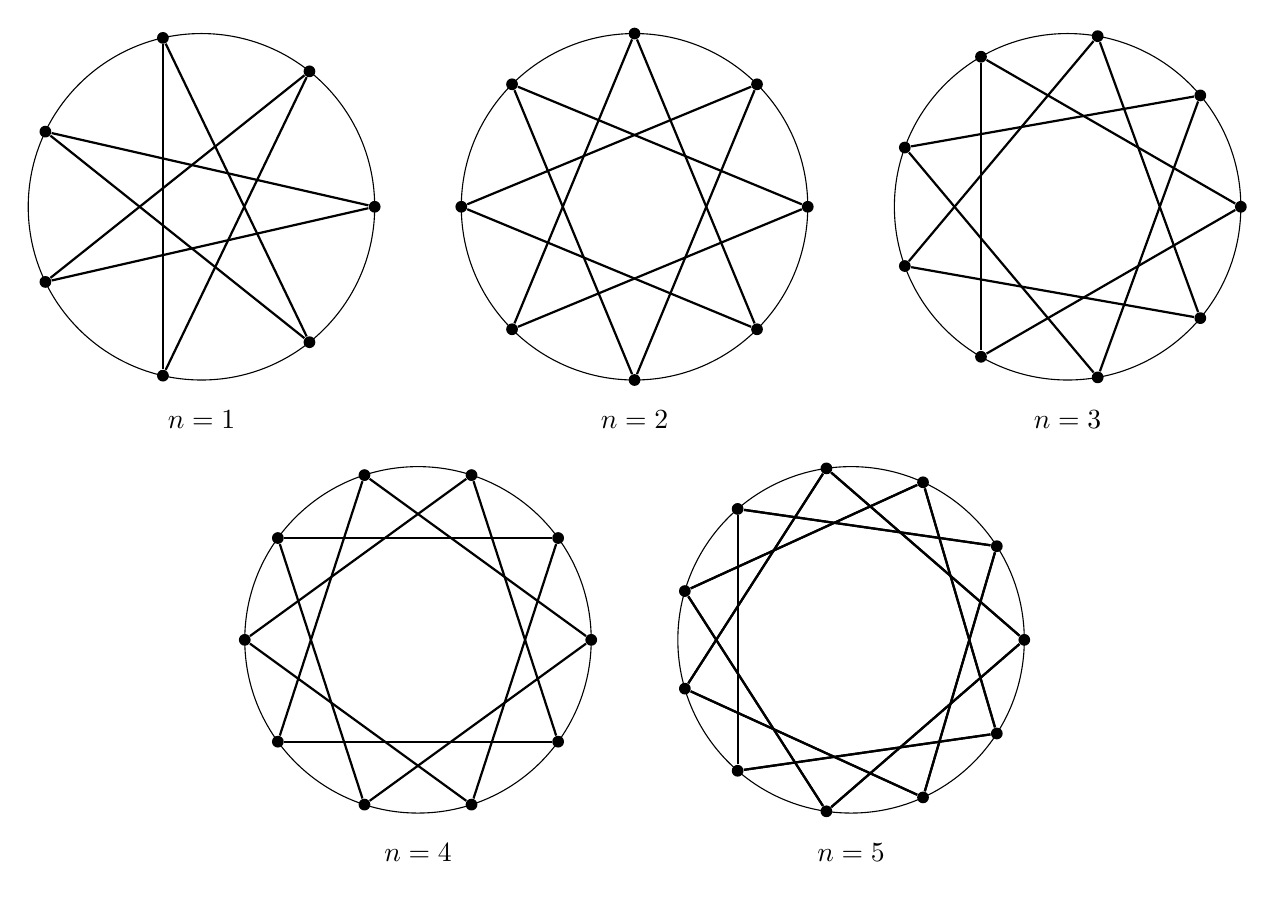
\begin{tikzpicture}[dot/.style={circle,fill=black,inner sep=1.5pt},line/.style={thick}
					] 
				\begin{scope}[xshift=0cm]
					 \def\skip{3}
					\draw (0,0) circle (2.2cm); 
					\foreach \i in {1,...,7}{ 
						\node[dot] (p\i)  at ({360/7 * (\i - 1)}:2.2cm) {};
					} 
					\foreach  \i in {1,...,7}{
						\pgfmathtruncatemacro{\j}{mod (\i + \skip  - 1,7) + 1}
						\draw[line] (p\i) --  (p\j);
					} 
					\node  at (0,-2.2cm - 0.5cm) {$n=1$};
				\end{scope}
				\begin{scope}[xshift=5.5cm]
					\def\skip{3} 
					\draw (0,0)  circle (2.2cm);
					\foreach \i in {1,...,8}{ 
						\node[dot] (p\i) at  ({360/8 * (\i - 1)}:2.2cm) {};
					 }
					\foreach  \i in {1,...,8}{
						\pgfmathtruncatemacro{\j}{mod (\i + \skip  - 1,8) + 1}
						\draw[line] (p\i)  -- (p\j);
					 }
					 \node at (0,-2.2cm - 0.5cm) {$n=2$};
				\end{scope}
				\begin{scope}[xshift=11cm]
					 \def\skip{3}
					\draw (0,0) circle (2.2cm); 
					\foreach  \i in {1,...,9}{
						\node[dot] (p\i) at ({360/9 * (\i - 1)}:2.2cm)  {};
					} 
					\foreach \i in {1,...,9}{ 
						\pgfmathtruncatemacro{\j}{mod  (\i + \skip - 1,9) + 1}
						 \draw[line] (p\i) -- (p\j);
					} 
					\node at (0,-2.2cm - 0.5cm)  {$n=3$};
				\end{scope}
				\begin{scope}[yshift=-5.5cm,xshift=2.75cm]
					\begin{scope}[xshift=0cm]
						 \def\skip{3}
						\draw (0,0) circle (2.2cm); 
						\foreach \i in {1,...,10}{ 
						\node[dot] (p\i) at ({360/10 * (\i  - 1)}:2.2cm) {};
						 }
						\foreach \i  in {1,...,10}{
						 \pgfmathtruncatemacro{\j}{mod (\i + \skip - 1,10) + 1}
						\draw[line] (p\i)  -- (p\j);
						} 
						\node at (0,-2.2cm - 0.5cm) {$n=4$}; 
					\end{scope}
					\begin{scope}[xshift=5.5cm]
						\draw (0,0) circle  (2.2cm);
						\foreach \i in  {1,...,11}{
						\node[dot] (p\i)  at ({360/11 * (\i - 1)}:2.2cm) {};
						 }
						\def\skipA{3} 
						\foreach  \i in {1,...,11}{
						\pgfmathtruncatemacro{\j}{mod (\i +  \skipA - 1,11) + 1}
						\draw[line] (p\i) -- (p\j); 
						 }
						\def\skipB{3} 
						\foreach \i  in {1,...,11}{
						\pgfmathtruncatemacro{\j}{mod (\i + \skipB - 1,11) +  1}
						\draw[line]  (p\i) -- (p\j);
						 }
						 \node at (0,-2.2cm - 0.5cm) {$n=5$};
					\end{scope}
				\end{scope}
			\end{tikzpicture}
	\end{center}
	 \shortans{90}
	\loigiai{ 
		Ta  thấy đường tròn được chia thành $n+6$ cung bằng nhau và mỗi cung có số đo bằng $\left(\dfrac{360}{n+6}\right)^\circ$.\\
		Do mỗi điểm  được nối với điểm cách nó hai điểm trên đường tròn nên góc ở đỉnh của mỗi ngôi sao là góc nội tiếp chắn $n+6 - 2 \cdot 3 = n$ cung bằng nhau đó.\\
		Suy ra số đo góc ở đỉnh tính theo đơn vị độ của mỗi ngôi sao là\\ $u_n = \dfrac{1}{2} \cdot \dfrac{360}{n+6} \cdot n = \dfrac{180n}{n+6} \xrightarrow{n=6} u_6  = 90^\circ$.
	} 
\end{ex}

% nguồn: Ok_TraLoiNgan_Lop11_Lan2
\begin{ex}%[1D2V1-3]%[ma:32104df6]
	Cho dãy số $(u_n)$ với $u_n=\dfrac{2n+1}{n-2}$. Hỏi dãy số đã cho có bao nhiêu số hạng  nguyên?
	\shortans{3} 
	 \loigiai{
		Ta  có $u_n=2+\dfrac{5}{n-2}$.\\
		$u_n$ là số nguyên khi $\dfrac{5}{n-2}$ là  số nguyên.\\
		 Khi đó $\hoac{&n-2=\pm1\\&n-2=\pm5}\Leftrightarrow\hoac{&n=3\\&n=1\\&n=7\\&n=-3.}$\\
		Vì $n\in\mathbb{N}^*$ nên có $3$ giá trị của  $n$ thỏa mãn. Vậy dãy số có $3$ số hạng là số nguyên.
	} 
\end{ex}

% nguồn: Ok_TraLoiNgan_Lop11_Lan2
\begin{ex}%[1D2V1-3]%[ma:1f9c31c4]
	Cho dãy số $(u_n)$  với $u_n=\dfrac{11n-10}{n+1}$, $\forall n\in\mathbb{N}^*$. Hỏi từ số hạng thứ mấy của dãy số $(u_n)$ thì các số hạng của dãy số lớn $10$?
	 \shortans{111}
	 \loigiai{
		Ta có  $u_n>10\Leftrightarrow\dfrac{11n-100}{n+1}>10\Leftrightarrow11n-100>10n+10\Leftrightarrow n>110$.\\
		Vậy từ số hạng thứ $111$ thì  các số hạng của dãy số lớn $10$.
	 }
\end{ex}

% nguồn: Ok_TraLoiNgan_Lop11_Lan2
\begin{ex}%[1D2V1-3]%[ma:bf45d05d]
	Cho dãy số  $(u_n)$ xác định bởi $\heva{&u_1=2021\\&u_{n+1}=\dfrac{u_n}{n}(n \geq 1)
	}$. Giá trị của  $2020!u_{2022}$ bằng bao nhiêu?
	 \shortans{1}
	\loigiai{Ta  có
		 \allowdisplaybreaks
		\begin{eqnarray*}
			u_n&=&\dfrac{u_{n-1}}{n-1}=\dfrac{u_{n-2}}{(n-1)(n-2)}=\dfrac{u_{n-3}}{(n-1)(n-2)(n-3)}\\ 
			&=&\ldots=\dfrac{u_1}{(n-1)(n-2)(n-3)\cdots2\cdot1}=\dfrac{u_1}{(n-1)!}, \forall n  \in \mathbb{N}; n \geq 2.
		\end{eqnarray*}
		 Do đó $u_{2022}=\dfrac{u_1}{2021!}=\dfrac{2021}{2021!}=\dfrac{1}{2020!}$.\\
		Vậy $2020!u_{2022}=1$. 
	} 
\end{ex}

% nguồn: Ok_TraLoiNgan_Lop11_Lan2
\begin{ex}%[1D2V1-3]%[ma:76fcdd06]
	Cho dãy số $(u_n)$ có $u_n=\dfrac{a  n+b}{n+1}$. Biết số hạng thứ $2$ và số hạng thứ $4$ lần lượt bằng $4$ và bằng $2$. Số hạng đầu tiên của dãy số bằng bao nhiêu?
	\shortans{6,5} 
	 \loigiai{
		 Vì $u_2=4$ và $u_4=2$ nên $\heva{&\dfrac{2a+b}{2+1}=4\\&\dfrac{4a+b}{4+1}=2} \Leftrightarrow\heva{&2a+b=12\\ &4a+b=10} \Leftrightarrow\heva{&a=-1\\&b=14.}$\\
		Do đó $u_n=\dfrac{-n+14}{n+1}$. Suy ra  $u_1=\dfrac{-1+14}{1+1}=\dfrac{13}{2}=6{,}5$.
	} 
\end{ex}

% nguồn: Ok_TraLoiNgan_Lop11_Lan2
\begin{ex}%[1D2V1-3]%[ma:282e4fd0]
	Cho hình vuông $A_1B_1C_1D_1$ có cạnh bằng $4$. Với mọi số nguyên dương $n \geq 2$, gọi $A_n$, $B_n$, $C_n$, $D_n$ lần lượt là trung điểm của các cạnh $A_{n-1}B_{n-1}$, $B_{n-1}C_{n-1}$,  $C_{n-1}D_{n-1}$, $D_{n-1}A_{n-1}$. Gọi $S_n$ là diện tích của tứ giác $A_nB_nC_nD_n$. Ta có $S_{12}=\dfrac{a}{b}$ với $a,\,b\in \mathbb{N}$ và $\dfrac{a}{b}$ là phân số tối giản. Giá trị của $T=a+\dfrac{1}{8}b$ bằng bao nhiêu?
	 \shortans{17}
	\loigiai{\begin{center}
		\begin{tikzpicture}
				\def\a{3} 
				\path (0:0)  coordinate (B_1)
					++(0:\a) coordinate  (C_1)
					++(90:\a) coordinate (D_1) 
					++(180:\a)  coordinate (A_1)
					 ($(A_1)!1/2!(B_1)$) coordinate (A_2)
					 ($(B_1)!1/2!(C_1)$) coordinate (B_2)
					 ($(C_1)!1/2!(D_1)$) coordinate (C_2)
					 ($(D_1)!1/2!(A_1)$) coordinate (D_2)
					 ($(A_2)!1/2!(B_2)$) coordinate (A_3)
					($(B_2)!1/2!(C_2)$) coordinate  (B_3)
					($(C_2)!1/2!(D_2)$) coordinate (C_3) 
					($(D_2)!1/2!(A_2)$) coordinate (D_3); 
				 \draw (A_1)--(B_1)--(C_1)--(D_1)--cycle
					 (A_2)--(B_2)--(C_2)--(D_2)--cycle
					(A_3)--(B_3)--(C_3)--(D_3)--cycle; 
				\foreach \x/ \goc in  {A_1/135,B_1/-135,C_1/-45,D_1/45,A_2/180,B_2/-90,C_2/0,D_2/90,A_3/-135,B_3/-45,C_3/45,D_3/135}
				\fill (\x) circle  (1pt)
					($(\x)+(\goc:3mm)$) node  {$\x$};
			\end{tikzpicture}
	\end{center}
	Ta thấy mỗi tứ giác $A_nB_nC_nD_n$ là một  hình vuông có cạnh là $A_nB_n$.\\
	Ta có $A_1B_1 = 4$, $A_2B_2 = \dfrac{1}{\sqrt{2}}A_1B_1 = 2\sqrt{2}$, $A_3B_3 = \dfrac{1}{\sqrt{2}}A_2B_2 = \left(\dfrac{1}{\sqrt{2}} \right)^2 A_1B_1 = 2$,$\ldots$\\  Tổng quát $A_nB_n = \left(\dfrac{1}{\sqrt{2}} \right)^{n-1}A_1B_1 = \left(\dfrac{1}{\sqrt{2}} \right)^{n-1}\cdot 4 = \left(\dfrac{1}{\sqrt{2}} \right)^{n-5}$.\\
	Diện tích hình vuông $A_nB_nC_nD_n$ là $S_n = \left(A_nB_n \right)^2 = \left(\dfrac{1}{2} \right)^{n-5}$, với mọi $n \in \mathbb{N}^*$.  \\
	Áp dụng với $n=12$ có $S_{12}  = \left(\dfrac{1}{2} \right)^{7} = \dfrac{1}{128}$.\\
	Suy ra  $a=1$, $b=128$.\\
Vậy $T=a+\dfrac{1}{8}b=1+\dfrac{1}{8}\cdot 128=17$.} 
\end{ex}

% nguồn: Ok_TraLoiNgan_Lop11_Lan2
\begin{ex}%[1D2V1-3]%[ma:169e974d]
	Cho dãy số $(u_n)$ xác định bởi  $\heva{&u_1=1\\
	&u_{n+1}=u_n+n^3, \forall n \in  \mathbb{N}^*
	}$. Số nguyên dương nhỏ nhất để $\sqrt{u_n-1} \geq 2\,039\,190$  bằng bao nhiêu?
	 \shortans{2020}
	\loigiai{Ta có  $\heva{&u_1=1\\
		 &u_2=u_1+1^3\\
		&u_3=u_2+2^3\\ 
		&\ldots \ldots \ldots \ldots \ldots \\ 
		 &u_{n}=u_{n-1}+\left(n-1\right)^3.}$\\
		Cộng vế theo vế  ta được\[u_1+u_2+u_3+\ldots+u_n=1+1^3+2^3+\ldots+\left(n-1\right)^2\Leftrightarrow u_n=1+1^3+2^3+\cdots+(n-1)^3.\]
		Ta  lại có $1^3+2^3+\cdots+(n-1)^3=(1+2+3+\cdots+n-1)^2=\left(\dfrac{n(n-1)}{2}\right)^2$.\\
		Suy ra $u_n=1+\left(\dfrac{n(n-1)}{2}\right)^2$.\\ 
		Theo  giả thiết ta có
		 \allowdisplaybreaks
		\begin{eqnarray*}
			\sqrt{u_n-1} \geq 2039190&\Leftrightarrow& \dfrac{n(n-1)}{2} \geq  2039190\\
			&\Leftrightarrow& n(n-1) \geq  4078380\\
			&\Leftrightarrow&\hoac{&n \geq 2020\\&n  \leq-2019.}
		\end{eqnarray*}
		Mà $n$ là số  nguyên dương nhỏ nhất nên $n=2020$.
	} 
\end{ex}

% nguồn: Ok_TraLoiNgan_Lop11_Lan2
\begin{ex}%[1D2V1-3]%[ma:95f5372c]
	Dãy số $(u_n)$ với $u_n=\dfrac{n^2-n+1}{n+2}$  có bao nhiêu số hạng là số nguyên?
	 \shortans{1}
	\loigiai{ 
		 Ta có $u_n=\dfrac{n^2-n+1}{+2}=n-3+\dfrac{7}{n+2}$.\\
		Vì  $n\in\mathbb{N}^*$ nên $u_n$ là số nguyên khi và chỉ khi $\dfrac{7}{n+2}$ là số nguyên.\\
		Khi đó  $\hoac{&n+2=1\\&n+2=-1\\&n+2=7\\&n+2=-7}\Leftrightarrow\hoac{&n=-1\\&n=-3\\&n=5\\&n=-9.}$\\
		Vì $n\in\mathbb{N}^*$ nên  chỉ có giá trị $n=5$ thõa mãn.\\
		Vậy dãy số $(u_n)$  có $1$ số hạng là số nguyên.
	} 
\end{ex}

% nguồn: Ok_TraLoiNgan_Lop11_Lan1
\begin{ex}%[1D2C1-3]%[ma:e0f2c1bf]
	Cho hình vuông $A_{1}B_{1}C_{1}D_{1}$ có cạnh bằng $4$. Với mọi số nguyên dương $n\geq 2$, gọi $A_{n}$, $B_{n}$; $C_{n}$, $D_{n}$ lần lượt là trung điểm của các cạnh $A_{n-1} B_{n-1}$, $B_{n-1} C_{n-1}$, $C_{n-1} D_{n-1}$, $D_{n-1} A_{n-1} $. Gọi $S_{n}$ là diện  tích của tứ giác $A_{n} B_{n} C_{n} D_{n}$. Biết $S_{12}=2^m$ với $m\in\mathbb{Z}$. Tính $m$.
	\shortans{-15} 
	 \loigiai{
		\begin{center}
			\begin{tikzpicture}[scale=1.2]
					 \coordinate (a1) at (0,4);
					\coordinate (c1)  at (4,0);
					\coordinate (b1) at  ($(a1)+(4,0)$);
					\coordinate (d1) at  ($(c1)-(4,0)$);
					 \draw (a1)--(b1)--(c1)--(d1)--cycle;
					\draw (a1) node[above]{$A_1$} 
						(b1)  node[above]{$B_1$}
						(c1) node[below]{$C_1$} 
						(d1)  node[below]{$D_1$};
					\coordinate (a2) at  (2,4);
					 \coordinate (c2) at (2,0);
					\coordinate (b2) at (4,2); 
					 \coordinate (d2) at (0,2);
					\draw (a2)--(b2)--(c2)--(d2)--cycle; 
					\draw (a2)  node[above]{$A_2$}
						 (b2) node[right]{$B_2$}
						(c2) node[below]{$C_2$} 
						 (d2) node[left]{$D_2$};
					\coordinate (a3) at  (3,3);
					 \coordinate (c3) at (1,1);
					 \coordinate (b3) at (3,1);
					 \coordinate (d3) at (1,3);
					\draw (a3)--(b3)--(c3)--(d3)--cycle; 
					\draw (a3) node[above  right]{$A_3$}
						(b3) node[below right]{$B_3$} 
						 (c3) node[below left]{$C_3$}
						(d3) node[above left]{$D_3$}; 
					 \coordinate (a4) at (3,2);
					 \coordinate (c4) at (1,2);
					\coordinate (b4) at  (2,1);
					\coordinate (d4) at  (2,3);
					\draw (a4)--(b4)--(c4)--(d4)--cycle; 
					\draw (a4)  node[right]{$A_4$}
						(b4)  node[below]{$B_4$}
						(c4)  node[left]{$C_4$}
						(d4)  node[above]{$D_4$};
				\end{tikzpicture}
		\end{center}
		Ta thấy mỗi tứ giác $A_{n} B_{n} C_{n} D_{n} $ là một hình vuông có cạnh là $A_{n}  B_{n} $.\\
		Ta có 
		$A_{1} B_{1} =4$, $A_{2} B_{2} =\dfrac{1}{\sqrt{2} } A_{1} B_{1} =2\sqrt{2}$, $A_{3} B_{3} =\dfrac{1}{\sqrt{2} } A_{2} B_{2} =\left(\dfrac{1}{\sqrt{2} } \right)^{2} A_{1} B_{1} =2$, $\ldots$\\ 
		Tổng quát: $A_{n} B_{n} =\left(\dfrac{1}{\sqrt{2} } \right)^{n-1} A_{1} B_{1} =\left(\dfrac{1}{\sqrt{2} } \right)^{n-1} \cdot 4=\left(\dfrac{1}{\sqrt{2} } \right)^{n+3} $.\\ 
		Diện tích hình vuông $A_{n}  B_{n} C_{n} D_{n}$ là $S_{n} =\left(A_{n} B_{n} \right)^{2} =\left(\dfrac{1}{2} \right)^{n+3} $,với mọi $n\in \mathbb{N}^{*}$.\\
	Áp dụng  với $n=12$ ta có $S_{12} =\left(\dfrac{1}{2} \right)^{15} =\dfrac{1}{32768}=2^{-15} \Rightarrow m=-15$.}
\end{ex}


%%%%%%%%%%%%%%%% TỰ LUẬN %%%%%%%%%%%%%%%%

% nguồn: Ok_TuanLuan_Toan11_Lan2
\begin{ex}%[1D2N1-3]%[ma:d3ba5d4f]
	Cho dãy số $(u_n)$ biết $u_n=\dfrac{1}{\sqrt{5}}\left[\left(\dfrac{1+\sqrt{5}}{2}\right)^n-\left(\dfrac{1-\sqrt{5}}{2}\right)^n\right]$. Tìm số hạng $u_6$. 
	 \loigiai{
		Ta có $u_6=\dfrac{1}{\sqrt{5}}\left[\left(\dfrac{1+\sqrt{5}}{2}\right)^6-\left(\dfrac{1-\sqrt{5}}{2}\right)^6\right]=8$. 
	} 
\end{ex}

% nguồn: Ok_TuanLuan_Toan11_Lan2
\begin{ex}%[1D2H1-3]%[ma:ffae4ea8]
	Một công ty dược phẩm đang thử nghiệm một loại thuốc mới. Một thí nghiệm bắt đầu với $1{,}0 \cdot 10^9 $ vi khuẩn. Một liều thuốc được sử dụng sau mỗi bốn giờ có thể tiêu diệt $ 4{,}0 \cdot 10^8 $ vi khuẩn. Giữa các liều thuốc, số lượng vi khuẩn  tăng lên $25\%$.
	\begin{enumerate}
		\item Viết hệ  thức truy hồi cho số lượng vi khuẩn sống trước mỗi lần sử dụng thuốc.
		\item Tìm số vi  khuẩn còn sống trước lần sử dụng thuốc thứ năm.
	\end{enumerate}
	 \loigiai{
		\begin{enumerate}
			\item Gọi $u_0 = 1,0 \cdot 10^9$ là số  vi khuẩn tại thời điểm ban đầu và $u_n$ là số vi khuẩn trước lần dùng thuốc thứ $n$.\\
			Do mỗi liều thuốc được sử dụng sau bốn giờ có thể tiêu diệt $4,0 \cdot 10^8$ vi khuẩn và giữa các  liều thuốc, số lượng vi khuẩn tăng lên $25\%$ nên ta có
			$$u_{n+1} = (u_n  - 4,0 \cdot 10^8) + 25\% u_n = 1,25u_n - 4,0 \cdot 10^8, \ \forall n \in \mathbb{N}^*.$$
			\item Ta  tính $u_5$ như sau:
			\begin{itemize}
				\item $u_1 = 1,0 \cdot 10^9$ 
				\item $u_2 = 1,25u_1  - 4,0 \cdot 10^8 = 8,5 \cdot 10^8$
				\item $u_3 = 1,25u_2 - 4,0 \cdot  10^8 = 6,625 \cdot 10^8$
				\item $u_4 = 1,25u_3 - 4,0 \cdot 10^8 = 4,28125 \cdot 10^8$ 
				 \item $u_5 = 1,25u_4 - 4,0 \cdot 10^8 = 1,3515625 \cdot 10^8$ .
			\end{itemize}
			Vậy số vi khuẩn  còn sống trước lần sử dụng thuốc thứ năm là $135\,156\,250$ con.
		\end{enumerate}
	 }
\end{ex}

% nguồn: Ok_TuanLuan_Toan11_Lan2
\begin{ex}%[1D2H1-3]%[ma:b3489ade]
	 Cho dãy số $(u_n)$ biết $\heva{&u_1=1\\&u_{n+1}=\dfrac{u_n+2}{u_n+1}}$. Tìm số hạng $u_{10}$.
	\loigiai{ 
		Ta  có
		\begin{enumEX}[$\bullet$]{2}
			 \item $u_2=\dfrac{u_1+2}{u_1+1}=\dfrac{1+2}{1+1}=\dfrac{3}{2}$.
			\item $u_3=\dfrac{u_2+2}{u_2+1}=\dfrac{\dfrac{3}{2}+2}{\dfrac{3}{2}+1}=\dfrac{7}{5}$. 
			\item  $u_4=\dfrac{u_3+2}{u_3+1}=\dfrac{\dfrac{7}{5}+2}{\dfrac{7}{5}+1}=\dfrac{17}{12}$.
			\item $u_5=\dfrac{u_4+2}{u_4+1}=\dfrac{\dfrac{17}{12}+2}{\dfrac{17}{12}+1}=\dfrac{41}{29}$. 
			\item  $u_6=\dfrac{u_5+2}{u_5+1}=\dfrac{\dfrac{41}{29}+2}{\dfrac{41}{29}+1}=\dfrac{99}{70}$.
			\item $u_7=\dfrac{u_6+2}{u_6+1}=\dfrac{\dfrac{99}{70}+2}{\dfrac{99}{70}+1}=\dfrac{239}{169}$. 
			 \item $u_8=\dfrac{u_7+2}{u_7+1}=\dfrac{\dfrac{239}{169}+2}{\dfrac{239}{169}+1}=\dfrac{577}{408}$.
			\item $u_9=\dfrac{u_8+2}{u_8+1}=\dfrac{\dfrac{577}{408}+2}{\dfrac{577}{408}+1}=\dfrac{1393}{985}$. 
			\item $u_{10}=\dfrac{u_9+2}{u_9+1}=\dfrac{\dfrac{1393}{985}+2}{\dfrac{1393}{985}+1}=\dfrac{3363}{2378}$. 
		\end{enumEX}
	 }
\end{ex}

% nguồn: Ok_TuanLuan_Toan11_Lan2
\begin{ex}%[1D2H1-3]%[ma:9f1b7e2a]
	Cho dãy số $(u_n)$ được xác định như sau $\heva{&u_1=1; u_2=2\\&u_{n+2}=2u_{n+1}+3u_n+5}$.  Tìm số hạng $u_8$.
	 \loigiai{
		Ta có 
		\begin{multicols}{2}
			\begin{itemize}
				\item  $u_3=2 u_2+3 u_1+5=12$.
				 \item $u_4=2 u_3+3 u_2+5=35$.
				\item $u_5=2 u_4+3 u_3+5=111$. 
				\item  $u_6=2 u_5+3 u_4+5=332$.
				\item  $u_7=2 u_6+3 u_5+5=1002$.
				 \item $u_8=2 u_7+3 u_6+5=3005$.
			\end{itemize}
		\end{multicols}
	 }
\end{ex}

% nguồn: Ok_TuanLuan_Toan11_Lan2
\begin{ex}%[1D2H1-3]%[ma:f644df67]
	Cho dãy số $(u_n)$ có số hạng tổng quát $u_n=\dfrac{2n+1}{n+2}$. Số $\dfrac{167}{84}$  là số hạng thứ mấy?
	\loigiai{ 
		Giả sử $u_n=\dfrac{167}{84} \Leftrightarrow \dfrac{2n+1}{n+2}=\dfrac{167}{84} \Leftrightarrow  84(2n+1)=167(n+2) \Leftrightarrow n=250$.\\
		Vậy $\dfrac{167}{84}$ là số hạng thứ $250$ của dãy số $(u_n)$. 
	} 
\end{ex}

% nguồn: Ok_TuanLuan_Toan11_Lan2
\begin{ex}%[1D2H1-3]%[ma:29bed381]
	Viết năm số hạng đầu và số hạng thứ $100$ của mỗi dãy số $(u_n)$ có số hạng tổng quát cho bởi công thức sau: 
	\begin{listEX}[3]
		\item  $u_n=3n-2$;
		 \item $u_n=3\cdot2^n$;
		 \item $u_n=\left(1+\dfrac{1}{n}\right)^n$.
	\end{listEX}
	\loigiai{ 
		\begin{listEX}[1]
			\item[a)] $u_1=1$; $u_2=4$; $u_3=7$; $u_4=10$;  $u_5=13$; $u_{100}=298$.
			 \item[b)] $u_1=6$; $u_2=12$; $u_3=24$; $u_4=48$; $u_5=96$; $u_{100}=3\cdot2^{100}$.
			 \item[c)] $u_1=2$; $u_2=\dfrac{9}{4}$; $u_3=\dfrac{64}{27}$; $u_4=\dfrac{625}{256}$; $u_5=\dfrac{7776}{3125}$; $u_{100}=\left(\dfrac{101}{100}\right)^{100}$.
		\end{listEX}
	} 
\end{ex}

% nguồn: Ok_TuanLuan_Toan11_Lan2
\begin{ex}%[1D2H1-3]%[ma:dbd27b4d]
	Cho dãy  số $(u_n)$ được xác định như sau $\heva{&u_1=1\\&u_{n+1}=u_n+2}$. Tìm số hạng $u_{50}$.
	 \loigiai{
		 Ta có
		\begin{itemize}
			 \item $u_1=1$.
			 \item $u_2=u_1+2$.
			\item $u_3=u_2+2$. 
			\item  $\ldots$.
			 \item $u_{50}=u_{49}+2$.
		\end{itemize}
		Cộng  theo vế các đẳng thức trên, ta được $u_{50}=1+2.49=99$.
	 }
\end{ex}

% nguồn: Ok_TuanLuan_Toan11_Lan2
\begin{ex}%[1D2H1-3]%[ma:fbcf3afc]
	Xét tính bị chặn của mỗi dãy  số $ (u_n)$ cho bởi công thức số hạng tổng quát như sau:
	\begin{enumEX}[a)]{2}
		\item  $ u_n = \dfrac{n^2 + 2n}{n^2 + n + 1} $.
		\item $ u_n = \dfrac{n}{\sqrt{n^2 + 2n + n}}  $.
		\item $u_n  = (-1)^n \cos\left( \dfrac{\pi}{2n} \right) $.
		\item $ u_n  = \dfrac{4\sin n + 4\cos(3n^2 + 1)}{5n^2 + n} $.
	\end{enumEX}
	 \loigiai{
		\begin{enumerate}
			\item $ u_n  = \dfrac{n^2 + 2n}{n^2 + n + 1} = 1 + \dfrac{n - 1}{n^2 + n + 1} $.\\
			Do $ 0 \le \dfrac{n - 1}{n^2  + n + 1} < 1, \ \forall n \in \mathbb{N}^* $.\\
			Suy ra $1 \le u_n  < 2, \ \forall n \in \mathbb{N}^* $.\\
			Vậy dãy số đã cho bị chặn. 
			\item $ u_n = \dfrac{n}{\sqrt{n^2  + 2n + n}} = \dfrac{1}{\sqrt{1 + \dfrac{2}{n} + \dfrac{1}{n^2}}} \Rightarrow 0 < u_n < \dfrac{1}{\sqrt{1 + \dfrac{2}{n} + \dfrac{1}{n^2}}} < \dfrac{1}{\sqrt{1}} = 1 $\\
			Suy ra $ 0 < u_n < 1,  \ \forall n \in \mathbb{N}^*$.\\ Vậy dãy số đã cho bị chặn.
			\item $ u_n = (-1)^n \cos\left(\dfrac{\pi}{2n}\right) \Rightarrow |u_n| =  \left|\cos\left(\dfrac{\pi}{2n}\right)\right| \le 1 \Rightarrow -1 \le u_n \le 1, \ \forall n \in \mathbb{N}^* $.\\
			Vậy dãy số đã cho bị chặn. 
			\item $ u_n = \dfrac{4\sin n  + 3\cos(3n^2 + 1)}{5n^2 + n}$.\\ $\Rightarrow |u_n| = \left| \dfrac{4\sin n + 3\cos(3n^2 + 1)}{5n^2 + n} \right| \le \dfrac{4|\sin n| + 3|\cos(3n^2 + 1)|}{5n^2 + n} $
			$ \le \dfrac{4 +  3}{5n^2 + n} = \dfrac{7}{5n^2 + n} < \dfrac{7}{5n^2} < \dfrac{7}{5n^2} ~\text{tiến đến}~ 0 \ \text{khi} \ n ~\text{tiến đến}~ \infty $
			$ \Rightarrow -1 < u_n < 1, \ \forall  n \in \mathbb{N}^*$.\\
			Vậy dãy số đã cho  bị chặn.
		\end{enumerate}
	} 
\end{ex}

% nguồn: Ok_TuanLuan_Toan11_Lan2
\begin{ex}%[1D2H1-3]%[ma:bd66d430]
	Cho dãy số $(u_n)$ được xác định bởi $\heva{&u_1=\dfrac{1}{2} \\ &u_{n+1}=u_n+2n}$.  Tìm số hạng $u_{50}$.
	 \loigiai{
		Ta có 
		\begin{itemize}
			\item  $u_1=\dfrac{1}{2}$.
			 \item $u_2=u_1+2.2$.
			\item $u_3=u_2+2.3$. 
			\item  $\ldots$.
			\item $u_{50}=u_{49}+2.50$. 
		\end{itemize}
		 Cộng theo vế các đẳng thức trên, ta được $u_{50}=\dfrac{1}{2}+2 \cdot(2+3+\cdots+50)=2548{,}5$.
	} 
\end{ex}

% nguồn: Ok_TuanLuan_Toan11_Lan2
\begin{ex}%[1D2H1-3]%[ma:ff36264b]
	Cho dãy số $(u_n)$ với $u_n=\dfrac{n^2+3n+7}{n+1}$.  Viết năm số hạng đầu tiên của dãy số đó.
	 \loigiai{
		Năm số hạng đầu tiên của dãy  số $(u_n)$ là
		\begin{eqnarray*}
			 &&u_1=\dfrac{1^2+3\cdot1+7}{1+1}=\dfrac{11}{2}. \\
			&&u_2=\dfrac{2^2+3\cdot2+7}{2+1}=\dfrac{17}{3}.  \\
			 &&u_3=\dfrac{2^2+3\cdot3+7}{3+1}=\dfrac{25}{4}. \\
			&&u_4=\dfrac{4^2+3\cdot4+7}{4+1}=7. \\ 
			 &&u_5=\dfrac{5^2+3\cdot5+7}{5+1}=\dfrac{47}{6}.
		\end{eqnarray*}
	} 
\end{ex}

% nguồn: Ok_TuanLuan_Toan11_Lan2
\begin{ex}%[1D2H1-3]%[ma:935d3998]
	Cho dãy số $(u_n)$ được xác định như sau $\heva{&u_1=0\\&u_{n+1}=\dfrac{n}{n+1}(u_n +1)}$.  Tìm số hạng $u_{11}$.
	\loigiai{ 
		Ta  có
		\begin{multicols}{2}
			\begin{itemize}
				\item  $u_2=\dfrac{1}{2}\left(u_1+1\right)=\dfrac{1}{2}$.
				\item $u_3=\dfrac{2}{3}\left(u_2+1\right)=1$. 
				\item $u_4=\dfrac{3}{4}\left(u_3+1\right)=\dfrac{3}{2}$. 
				\item  $u_5=\dfrac{4}{5}\left(u_4+1\right)=2$.
				\item  $u_6=\dfrac{5}{6}\left(u_5+1\right)=\dfrac{5}{2}$.
				\item  $u_7=\dfrac{6}{7}\left(u_6+1\right)=3$.
				\item $u_8=\dfrac{7}{8}\left(u_7+1\right)=\dfrac{7}{2}$. 
				 \item $u_9=\dfrac{8}{9}\left(u_8+1\right)=4$.
				\item $u_{10}=\dfrac{9}{10}\left(u_9+1\right)=\dfrac{9}{2}$. 
				 \item $u_{11}=\dfrac{10}{11}\left(u_{10}+1\right)=5$.
			\end{itemize}
		\end{multicols}
	 }
\end{ex}

% nguồn: Ok_TuanLuan_Toan11_Lan2
\begin{ex}%[1D2H1-3]%[ma:4cb405ae]
	Viết  năm số hạng đầu tiên của mỗi dãy số $(u_n)$ sau:
	\begin{listEX}[2]
		\item $u_n=(-1)^{n+1} \cdot  n^2$;
		\item $\heva{&u_1=1, \; u_2=2  \\ &u_n=u_{n-1} \cdot u_{n-2}, \; n \ge 3.}$
	\end{listEX}
	 \loigiai{
		\begin{listEX}[1]
			\item Thay lần lượt $n=1$, $2$, $3$, $4$, $5$ vào công thức của $u_n$ ta có 
			\begin{eqnarray*}
				&&u_1=(-1)^2  \cdot 1^2=1. \\
				&&u_2=(-1)^3 \cdot 2^2=-4. \\ 
				 &&u_3=(-1)^4 \cdot 3^2=9. \\
				&&u_4=(-1)^5 \cdot 4^2=-16. \\ 
				 &&u_5=(-1)^6 \cdot 5^2=25.
			\end{eqnarray*}
			 \item Thay lần lượt $n=3$, $4$, $5$ vào công thức của $u_n$ ta có
			\begin{eqnarray*}
				 &&u_1=1, \; u_2=2 \\
				&&u_3=u_1 \cdot u_2=1 \cdot  2=2. \\
				&&u_4=u_3 \cdot u_2=2  \cdot 2=4. \\
				 &&u_5=u_4 \cdot u_3=4 \cdot 2=8.
			\end{eqnarray*}
		\end{listEX}
	} 
\end{ex}

% nguồn: Ok_TuanLuan_Toan11_Lan2
\begin{ex}%[1D2H1-3]%[ma:83b0cd82]
	Thực hiện các yêu cầu của bài toán trong mỗi trường hợp dưới đây. 
	\begin{listEX}[1]
		\item Cho dãy số $(u_n)$ biết $\heva{&u_1=1 \\ &u_{n+1}=\dfrac{u_n+2}{u_n+1}, \; n \ge  2.}$ \\
		Hãy tìm số  hạng $u_{10}$.
		\item Cho dãy số $(u_n)$ được xác định  như sau $\heva{&u_1=1 \\ &u_{n+1}=u_n+2, \; n \ge 2.}$ \\
		Hãy tìm  số hạng $u_{50}$.
		\item Cho dãy  số $(u_n)$ được xác định như sau $\heva{&u_1=1, \; u_2=2 \\ &u_{n+2}=2u_{n+1}+3u_n+5, \; n \ge 3.}$ \\
		Hãy tìm số hạng  $u_8$.
		\item Cho dãy số $(u_n)$ được xác định như sau $\heva{&u_1=0 \\ &u_{n+1}=\dfrac{n}{n+1} \cdot \left(u_n+1\right),  \; n \ge 2.}$ \\
		Hãy  tìm số hạng $u_{11}$.
	\end{listEX}
	\loigiai{ 
		\begin{listEX}[1]
			\item Ta có 
			\begin{eqnarray*}
				 &&u_2=\dfrac{u_1+2}{u_1+1}=\dfrac{3}{2}. \\
				 &&u_3=\dfrac{u_2+2}{u_2+1}=\dfrac{7}{5}. \\
				&&u_4=\dfrac{u_3+2}{u_3+1}=\dfrac{17}{12}. \\ 
				 &&u_5=\dfrac{u_4+2}{u_4+1}=\dfrac{41}{29}. \\
				&&u_6=\dfrac{u_5+2}{u_5+1}=\dfrac{99}{70}.  \\
				 &&u_7=\dfrac{u_6+2}{u_6+1}=\dfrac{239}{169}. \\
				&&u_8=\dfrac{u_7+2}{u_7+1}=\dfrac{577}{408}.  \\
				&&u_9=\dfrac{u_8+2}{u_8+1}=\dfrac{1393}{985}.  \\
				 &&u_{10}=\dfrac{u_9+2}{u_9+1}=\dfrac{3363}{2378}.
			\end{eqnarray*}
			\item Từ giả  thiết ta có
			 $$u_1=1, \; u_2=u_1+2, \; u_3=u_2+2, \; \ldots, \; u_{50}=u_{49}+2.$$
			Cộng theo vế các đẳng thức  trên ta được
			 \allowdisplaybreaks
			\begin{eqnarray*}
				 &&u_1+u_2+\cdots+u_{50}=1+u_1+2+u_2+2+\cdots+u_{49}+2\\
				&\Leftrightarrow& u_{50}=1+2 \cdot  49=99.
			\end{eqnarray*}
			\item Ta  có
			\begin{eqnarray*}
				 &&u_3=2u_2+3u_1+5=12. \\
				&&u_4=2u_3+3u_2+5=35.  \\
				&&u_5=2u_4+3u_3+5=111.  \\
				 &&u_6=2u_5+3u_4+5=332. \\
				&&u_7=2u_6+3u_5+5=1002.  \\
				&&u_8=2u_7+3u_6+5=3005. 
			\end{eqnarray*}
			\item Ta có 
			\begin{eqnarray*}
				 &&u_1=0. \\
				 &&u_2=\dfrac{1}{2} \cdot \left(u_1+1\right)=\dfrac{1}{2}. \\
				&&u_3=\dfrac{2}{3} \cdot  \left(u_2+1\right)=1. \\
				 &&u_4=\dfrac{3}{4} \cdot \left(u_3+1\right)=\dfrac{3}{2}. \\
				&&u_5=\dfrac{4}{5} \cdot \left(u_4+1\right)=2.  \\
				&&u_6=\dfrac{5}{6} \cdot \left(u_5+1\right)=\dfrac{5}{2}. \\ 
				&&u_7=\dfrac{6}{7} \cdot \left(u_6+1\right)=3. \\ 
				&&u_8=\dfrac{7}{8}  \cdot \left(u_7+1\right)=\dfrac{7}{2}. \\
				&&u_9=\dfrac{8}{9} \cdot \left(u_8+1\right)=4.  \\
				&&u_{10}=\dfrac{9}{10} \cdot  \left(u_9+1\right)=\dfrac{9}{2}. \\
				&&u_{11}=\dfrac{10}{11} \cdot \left(u_{10}+1\right)=5. 
			\end{eqnarray*}
		\end{listEX}
	 }
\end{ex}

% nguồn: Ok_TuanLuan_Toan11_Lan2
\begin{ex}%[1D2C1-3]%[ma:609cbd89]
	Cho $S=1\cdot 2+3\cdot 4+5\cdot 6+\cdots+(2n-1)\cdot 2n$. Tính $S_{100}$ biết  rằng
	 \[\sum\limits_{i=1}^n 2i=2+4+6+\cdots+2n=n(n+1);\sum\limits_{i=1}^n i^2=1+2^2+3^2+\cdots+n^2=\dfrac{n(n+1)(2n+1)}{6}.\]
	\loigiai{ 
		 Ta có
		\begin{align*}
			S&=\sum\limits_{i=1}^n  2i(2i-1)=\sum\limits_{i=1}^n(4i^2-2i)\\
			&=4\sum\limits_{i=1}^n i^2-2\sum\limits_{i=1}^n i=4\dfrac{n(n+1)(2n+1)}{6}-n(n+1)=\dfrac{n(n+1)(4n-1)}{3}.\\ 
			S_{100}&=\dfrac{100\cdot(100+1)(4\cdot  100-1)}{3}=1343300
		\end{align*}
	} 
\end{ex}

% nguồn: Ok_TuanLuan_Toan11_Lan2
\begin{ex}%[1D2C1-3]%[ma:f83e12a2]
	Cho tổng $S_n=1\cdot 4+2\cdot 7+3\cdot 10+\cdots+n\cdot(3n+1)$ với $n\in\mathbb{N}^*$. Biết $S_k=294$. Giá  trị của $k$ là
	\loigiai{ 
		Ta có $S_n=\sum\limits_{i=1}^n(3i+1)=\sum\limits_{i=1}^n(3i^2+i)=3\sum\limits_{i=1}^n i^2+\sum\limits_{i=1}^n i=3\dfrac{n(n+1)(2n+1)}{6}+\dfrac{n(n+1)}{2}=n(n+1)^2$.\\ 
		$\Rightarrow S_k=k(k+1)^2=294\Leftrightarrow k^3+2k^2+k=294\Leftrightarrow(k-6)(k^2+8k+49)=0\Leftrightarrow  k=6$.
	 }
\end{ex}

% nguồn: Ok_TuanLuan_Toan11_Lan2
\begin{ex}%[1D2C1-3]%[ma:e277c43a]
	 Tính tổng$S= \left( 1-\dfrac{1}{2}\right)+\left(1-\dfrac{1}{4}\right)+\left(1-\dfrac{1}{8}\right)+\cdots+\left(1-\dfrac{1}{2^n}\right)$. Tính $S_{10}$.
	 \loigiai{
		\begin{itemize}
			\item Giải theo phương pháp tự luận 
			\begin{itemize}
				 \item \textbf{Cách 1}
				Ta có 
				\begin{align*}
					S_{10}&=\left(  1-\dfrac{1}{2}\right)+\left(1-\dfrac{1}{2^2}\right)+\left(1-\dfrac{1}{2^3}\right)+\cdots+\left(1-\dfrac{1}{2^{10}}\right)\\
					&=10-\left( \dfrac{1}{2}+\dfrac{1}{2^2}+\dfrac{1}{2^3}+\cdots+\dfrac{1}{2^{10}}\right) 
				\end{align*}
				Đặt$M=\dfrac{1}{2}+\dfrac{1}{2^2}+\dfrac{1}{2^3}+\cdots+\dfrac{1}{2^{10}}$. 
				Ta có 
				\begin{align*}
					2M&=1+\dfrac{1}{2}+\dfrac{1}{2^2}+\cdots+\dfrac{1}{2^9}\\ 
					\Rightarrow 2M-M &= \left( 1+\dfrac{1}{2}+\dfrac{1}{2^2}+\cdots+\dfrac{1}{2^9}\right) -\left(  \dfrac{1}{2}+\dfrac{1}{2^2}+\dfrac{1}{2^3}+\cdots+\dfrac{1}{2^{10}}\right) \dfrac{1}{2}+\dfrac{1}{2^2}+\dfrac{1}{2^3}+\cdots+\dfrac{1}{2^{10}}\\
					M&=1-\dfrac{1}{2^{10}} 
				\end{align*}
				Suy ra $  S=10-\left( 1-\dfrac{1}{2^{10}}\right) =9+\dfrac{1}{2^{10}}$.
				\item  \textbf{Cách 2}
				Ta có $S_n=n-\left(  \dfrac{1}{2}+\dfrac{1}{2^2}+\dfrac{1}{2^3}+\cdots+\dfrac{1}{2^n}\right) $.
				Đặt$M=\dfrac{1}{2}+\dfrac{1}{2^2}+\dfrac{1}{2^3}+\cdots+\dfrac{1}{2^n}$. 
				 Ta có
				\begin{align*}
					 2M&=1+\dfrac{1}{2}+\dfrac{1}{2^2}+\cdots+\dfrac{1}{2^{n-1}}\\
					\Rightarrow 2M-M&=\left(  1+\dfrac{1}{2}+\dfrac{1}{2^2}+\cdots+\dfrac{1}{2^{n-1}}\right) 1+\dfrac{1}{2}+\dfrac{1}{2^2}+\cdots+\dfrac{1}{2^{n-1}}-\left( \dfrac{1}{2}+\dfrac{1}{2^2}+\dfrac{1}{2^3}+\cdots+\dfrac{1}{2^n}\right)
				\end{align*}
				Suy ra  $M =1-\dfrac{1}{2^n}$.
				Suy ra $ S_n=n-(1-\dfrac{1}{2^n})=n-1+\dfrac{1}{2^n}$. 
				Suy ra $\Rightarrow S_{10}=10-1+\dfrac{1}{2^{10}}=9+\dfrac{1}{2^{10}}$. 
			\end{itemize}
			 \item Giải theo phương pháp trắc nghiệm
			Ta  có
			\begin{align*}
				 S_{10}&=10-\left( \dfrac{1}{2}+\dfrac{1}{2^2}+\dfrac{1}{2^3}+\cdots+\dfrac{1}{2^{10}}\right) \\
				&=10- \frac{\frac{1}{2}\left(\left(\frac{1}{2}\right)^{10}-1\right)}{\frac{1}{2}-1} = 10-  \left(1- \dfrac{1}{2^{10}} \right) \\
				 &=10-1+\dfrac{1}{2^{10}}=9+\dfrac{1}{2^{10}}
			\end{align*}
			\item Giải theo  Casio
			Nhận xét  $S_n=n-\left( \dfrac{1}{2}+\dfrac{1}{2^2}+\dfrac{1}{2^3}+\cdots+\dfrac{1}{2^n}\right)$.
			Nhập máy  tính tổng $\dfrac{1}{2}+\dfrac{1}{2^2}+\dfrac{1}{2^3}+\cdots+\dfrac{1}{2^n}$ với số hạng tổng quát$u_n=\dfrac{1}{2^n}$, số số hạng$u_n=10$ ta được kết quả $\dfrac{1023}{1024}$.
			 Nhập tiếp$10-Ans$ được kết quả$\dfrac{9217}{1024}$.
			Ta gán$\dfrac{9217}{1024}\to  A$.
			Lấy từng kết quả ở 4 đáp án trừ cho A  khi nào bằng $0$ thì chọn đáp án đó.
		\end{itemize}
	} 
\end{ex}

% nguồn: Ok_TuanLuan_Toan11_Lan2
\begin{ex}%[1D2C1-3]%[ma:7e041ff7]
	Tính $S=1\cdot 3+2\cdot 5+3\cdot  7+\cdots+n(2n+1)$. Biết rằng
	\begin{align*}
		&\sum\limits_{i=1}^n  i=1+2+3+\cdots+n=\dfrac{n(n+1)}{2};\\
		 &\sum\limits_{i=1}^n i^2=1+2^2+3^2+\cdots+n^2=\dfrac{n(n+1)(2n+1)}{6}.
	\end{align*}
	\loigiai{ 
		$S=\sum\limits_{i=1}^n i(2i+1)=\sum\limits_{i=1}^n(2i^2+i)=2\sum\limits_{i=1}^n i^2+\sum\limits_{i=1}^n  i=2\dfrac{n(n+1)(2n+1)}{6}+\dfrac{n(n+1)}{2}=\dfrac{n(n+1)(4n+5)}{6}$.
	} 
\end{ex}
